
% !TEX root = main.tex
\documentclass{Setup/template_isec_class}

% Template ISEC/LaTeX, janeiro 2023
%--------------------------------------
\usepackage{Setup/template_isec_package}
%--------------------------------------

%--------------------------------------
% Obs#1
% Onde incluir todos os ficheiros (package)
% e instruções adicionais para este projeto
\usepackage{extras}
\usepackage{amsfonts}
\usepackage{amsmath}
\usepackage{amssymb}
\usepackage{algorithm}
\usepackage{algpseudocode}
%--------------------------------------

\begin{document}

%--------------------------------------
% Obs#2
% Definir qual o título e quais os autores do trabalho
\newcommand{\titulotrabalho}{Protein Structure and 2D Structure Prediction using Deep Reinforcement Learning}
\newcommand{\autorestrabalho}{Arbi Golemi}
%--------------------------------------

\pagestyle{empty}

% Capa
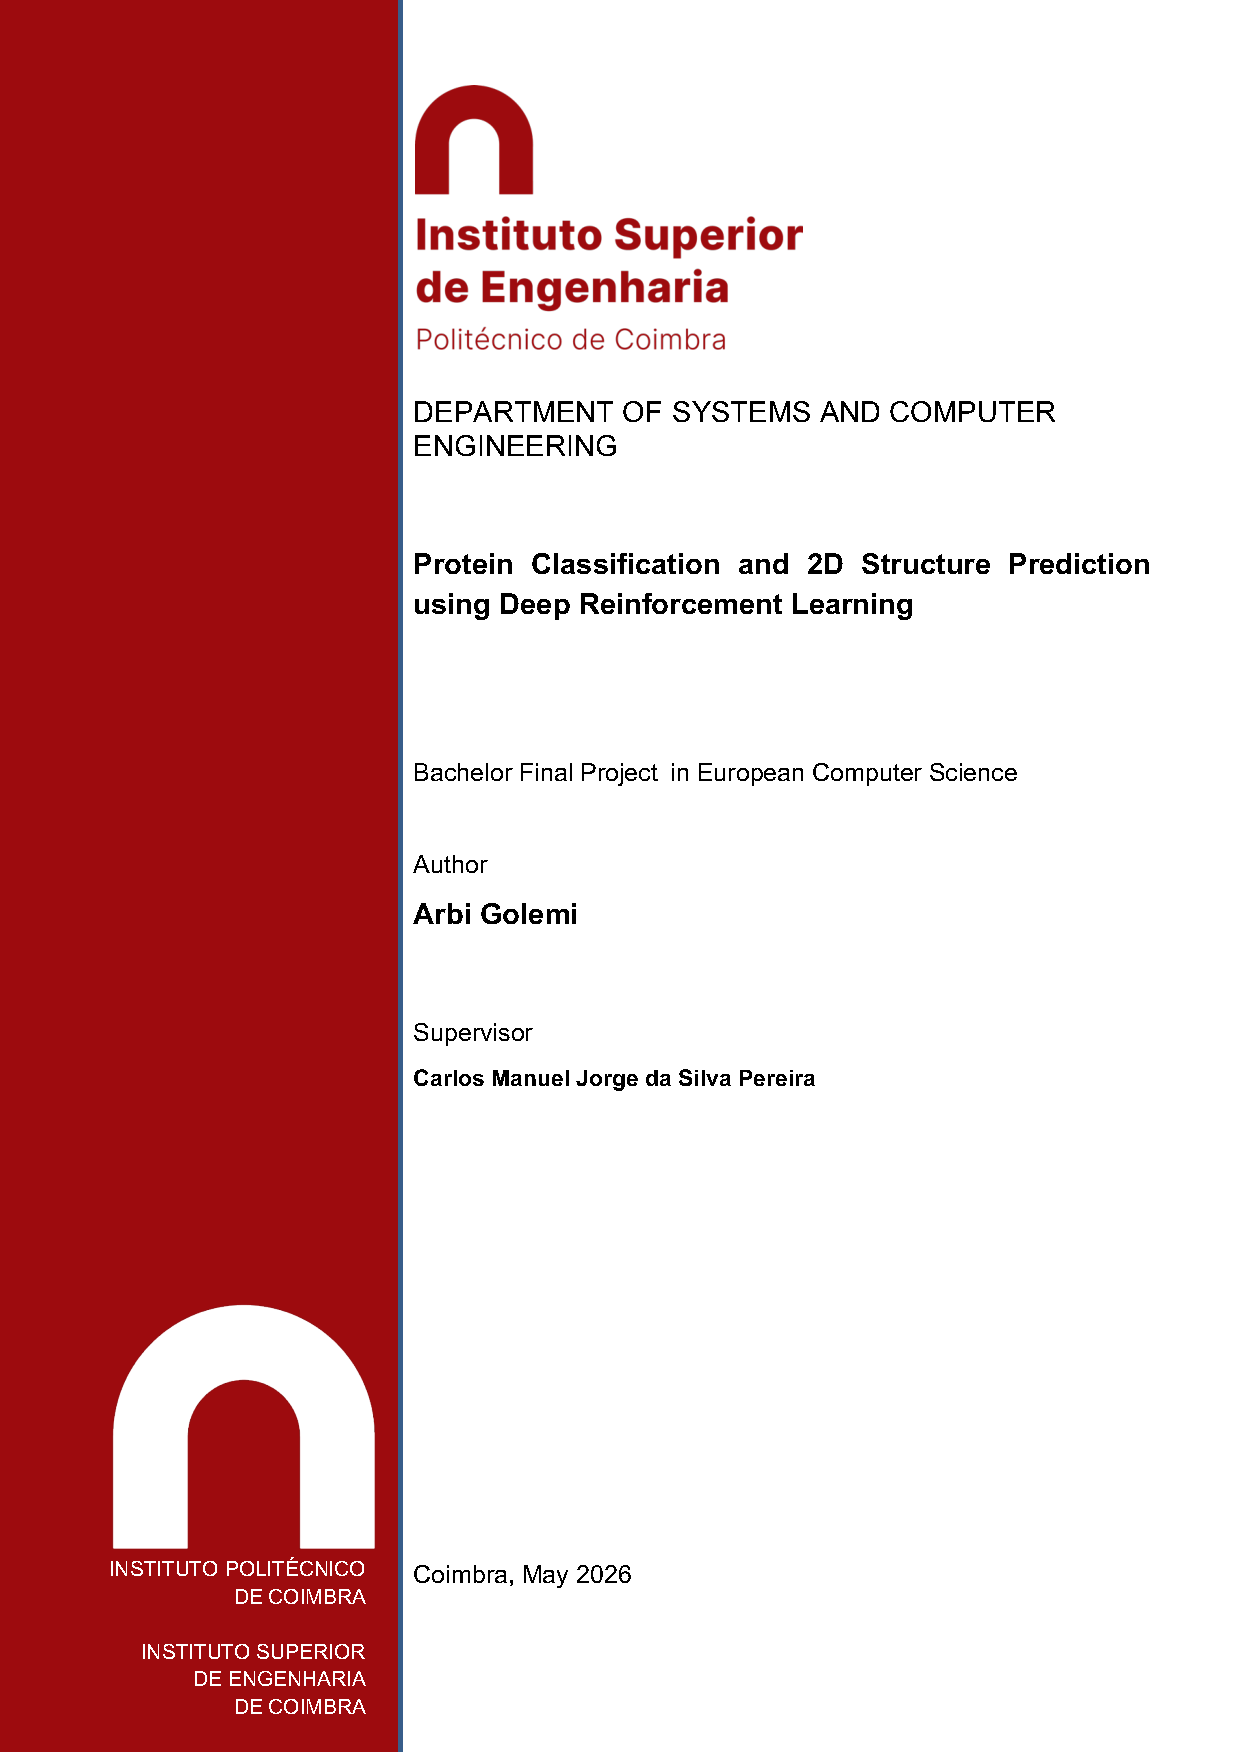
\includepdf{Inicio/capa}

\newpage

%--------------------------------------
\pagestyle{fancy}
\fancyhf{}
\fancyhead{}
\fancyhead[CO]{\nouppercase{\truncate{\headwidth}{\titulotrabalho}}}
\fancyhead[CE]{\nouppercase{\autorestrabalho}}
\renewcommand{\headrulewidth}{0pt}
\fancyfoot{}
\fancyfoot[CO,CE]{\thepage}
\setlength{\headheight}{14.5pt}
\fancypagestyle{plain}{}
%--------------------------------------

\pagenumbering{roman}

% Resumo PT
\phantomsection
\addcontentsline{toc}{chapter}{Resumo}
% !TEX root = ../main.tex
% Resumo
%--------------------------------------
\vspace*{45pt}
\begin{flushleft}
	{\Large \textbf{\scshape{Resumo}}}
\end{flushleft}
\vspace*{10pt}

A relação entre a sequência de aminoácidos de uma proteína e a sua estrutura tridimensional e função biológica é um foco central da biologia computacional moderna. Este projeto apresenta o desenvolvimento de uma plataforma web abrangente, construída com a framework Django, concebida para prever tanto a estrutura como as características funcionais das proteínas diretamente a partir de sequências FASTA. Para a anotação funcional, a plataforma integra a API DeepGO para prever os termos da Gene Ontology (GO), oferecendo um mapeamento rápido e acessível de sequência para função. Para abordar o complexo problema do enovelamento de proteínas, o estudo utiliza o modelo de rede 2D Hidrofóbico-Polar (HP). Um conjunto de algoritmos clássicos de otimização heurística  incluindo Hill Climbing, Simulated Annealing e Replica Exchange Monte Carlo  foi implementado e avaliado para estabelecer bases de referência estruturais. Com base nestes métodos clássicos, foram introduzidas técnicas de Inteligência Artificial para mapear trajetórias de enovelamento. A progressão do Tabular Q-Learning para uma Deep Q-Network (DQN) personalizada, baseada em PyTorch, demonstra a capacidade das Redes Neurais Convolucionais (CNNs) para aprender dependências espaciais dentro da grelha da proteína, superando as limitações dimensionais dos métodos tabulares. A plataforma resultante unifica estas diversas metodologias computacionais numa única interface, demonstrando a eficácia do Deep Reinforcement Learning na resolução de problemas complexos de otimização biofísica.

\vspace*{20pt}

\noindent \textbf{Palavras-chave}:
Enovelamento de Proteínas, Deep Reinforcement Learning, Django, Gene Ontology, Modelo HP.


\newpage

% Abstract ENG
\phantomsection
\addcontentsline{toc}{chapter}{Abstract}
% !TEX root = ../main.tex
% Abstract
%--------------------------------------
\vspace*{45pt}
\begin{flushleft}
	{\Large \textbf{\scshape{Abstract}}}
\end{flushleft}
\vspace*{10pt}

The relationship between a protein's amino acid sequence and its three-dimensional structure and biological function is a central focus of modern computational biology. This project presents the development of a comprehensive web-based platform, built with the Django framework, designed to predict both the structure and the functional characteristics of proteins directly from FASTA sequences. For functional annotation, the platform integrates the DeepGO API to predict Gene Ontology (GO) terms, offering rapid and accessible sequence-to-function mapping. To address the complex protein folding problem, the study utilizes the 2D Hydrophobic-Polar (HP) lattice model. A suite of classical heuristic optimization algorithms including Hill Climbing, Simulated Annealing, Monte Carlo, and Replica Exchange Monte Carlo was implemented and benchmarked to establish structural baselines. Building upon these classical methods, Artificial Intelligence techniques were introduced to map folding trajectories. The progression from Tabular Q-Learning to a custom PyTorch-based Deep Q-Network (DQN) demonstrates the capability of Convolutional Neural Networks (CNNs) to learn spatial dependencies within the protein grid, overcoming the dimensional limitations of tabular methods. The resulting platform unifies these diverse computational methodologies into a single interface, demonstrating the potential of Deep Reinforcement Learning for complex biophysical optimization problems.

\vspace*{20pt}

\noindent \textbf{Keywords}:
Protein Folding, Deep Reinforcement Learning, Django, Gene Ontology, HP Model.


\newpage

% Epígrafe
\phantomsection
\addcontentsline{toc}{chapter}{Ep\'{\i}grafe}

% Epígrafe
%--------------------------------------
\vspace*{45pt}
\begin{flushleft}
	{\Large \textbf{\scshape{Ep\'{\i}grafe}}}
\end{flushleft}
\vspace*{10pt}

\begin{flushright}
	Nothing in life is to be feared, it is only to be understood. Now is the time to understand more, so that we may fear less. \\
	Marie Curie
\end{flushright}



\newpage

% Dedicatória
\phantomsection
\addcontentsline{toc}{chapter}{Dedicat\'{o}ria}

% Dedicatória
%--------------------------------------
\vspace*{45pt}
\begin{flushleft}
	{\Large \textbf{\scshape{Dedication}}}
\end{flushleft}
\vspace*{10pt}

To my parents, who sacrificed so much of their lives to give me a better one. This achievement is for you.


Ai miei genitori, che hanno sacrificato tanto della loro vita per offrirmene una migliore. Questo traguardo è per loro.


Prindërve të mi, që sakrifikuan aq shumë nga jeta e tyre për të më dhënë mua një të ardhme më të mirë. Ky sukses është për ta.
% !TEX root = ../main.tex


\newpage

% Agradecimentos
\phantomsection
\addcontentsline{toc}{chapter}{Agradecimentos}

% Agradecimentos
%--------------------------------------
\vspace*{45pt}
\begin{flushleft}
	{\Large \textbf{\scshape{Agradecimentos}}}
\end{flushleft}
\vspace*{10pt}

I would first like to thank my supervisor for their availability, support, and valuable advice throughout the development of this work.

I would like to thank Ca’ Foscari University of Venice for the education I have received over the years and for giving me the opportunity to enrich my academic and personal journey. I would also like to thank all the professors who, through their teaching, contributed to my growth.

I would also like to thank the Polytechnic Institute of Coimbra and all the professors who, during this year, welcomed and guided me, contributing to my personal and professional development.

A special thanks goes to my family, especially my parents and my brother, for their love, sacrifices, and constant support, which allowed me to reach this milestone.

Finally, I would like to thank myself for the determination, patience, and strength to never give up in the face of difficulties.

\newpage

\renewcommand{\contentsname}{\'{I}ndice}
\renewcommand{\listtablename}{\'{I}ndice de tabelas}
\renewcommand{\listfigurename}{\'{I}ndice de figuras}

\phantomsection
\addcontentsline{toc}{chapter}{\'{I}ndice}
\tableofcontents

\newpage

\phantomsection
\addcontentsline{toc}{chapter}{\'{I}ndice de tabelas}
\listoftables

\newpage

\phantomsection
\addcontentsline{toc}{chapter}{\'{I}ndice de figuras}
\listoffigures

\newpage

% Lista de abreviaturas
\phantomsection
\addcontentsline{toc}{chapter}{Lista de abreviaturas}

% Lista de abreviaturas
%--------------------------------------
\vspace*{45pt}
\begin{flushleft}
	{\Large \textbf{\scshape{List of Abbreviations}}}
\end{flushleft}
\vspace*{20pt}

\begin{description}
    \item[2D] Two-dimensional
    \item[3D] Three-dimensional
    \item[AA] Amino acid
    \item[AI] Artificial Intelligence
    \item[API] Application Programming Interface
    \item[CNN] Convolutional Neural Network
    \item[CPU] Central Processing Unit
    \item[cryo-EM] Cryogenic Electron Microscopy
    \item[CSS] Cascading Style Sheets
    \item[CUDA] Compute Unified Device Architecture
    \item[DB] Database
    \item[DQN] Deep Q-Network
    \item[DRL] Deep Reinforcement Learning
    \item[FASTA] FAST-All sequence format
    \item[GO] Gene Ontology
    \item[GO:BP] Gene Ontology: Biological Process
    \item[GO:CC] Gene Ontology: Cellular Component
    \item[GO:MF] Gene Ontology: Molecular Function
    \item[GET] HTTP GET request method
    \item[GPU] Graphics Processing Unit
    \item[H] Hydrophobic residue
    \item[HC] Hill Climbing
    \item[HP] Hydrophobic-Polar
    \item[HTML] HyperText Markup Language
    \item[IEEE] \textit{Institute of Electrical and Electronics Engineers}
    \item[ISEC] Instituto Superior de Engenharia de Coimbra
    \item[JSON] JavaScript Object Notation
    \item[MC] Monte Carlo
    \item[MDP] Markov Decision Process
    \item[MSE] Mean Squared Error
    \item[MVT] Model-View-Template
    \item[NP] Nondeterministic Polynomial time
    \item[P] Polar residue
    \item[PDB] Protein Data Bank
    \item[POST] HTTP POST request method
    \item[PPO] Proximal Policy Optimization
    \item[QL] Q-Learning
    \item[REMC] Replica Exchange Monte Carlo
    \item[RL] Reinforcement Learning
    \item[RMSD] Root Mean Square Deviation
    \item[SA] Simulated Annealing
    \item[SAC] Soft Actor-Critic
    \item[SAW] Self-Avoiding Walk
    \item[SVG] Scalable Vector Graphics
    \item[TD] Temporal Difference
    \item[TM-score] Template Modelling score
    \item[UniProt] Universal Protein Resource
\end{description}
% !TEX root = ../main.tex


\newpage

% Lista de símbolos
\phantomsection
\addcontentsline{toc}{chapter}{Lista de s\'{\i}mbolos}

% Lista de símbolos
%--------------------------------------
\vspace*{45pt}
\begin{flushleft}
	{\Large \textbf{\scshape{List of Symbols}}}
\end{flushleft}
\vspace*{20pt}

\begin{description}
    \item[$a$] Action selected by the reinforcement learning agent
    \item[$a'$] Candidate or next action
    \item[$\mathcal{A}$] Action space
    \item[$\beta_k$] Inverse temperature of replica $k$, defined as $\beta_k = 1/T_k$
    \item[$\mathcal{C}$] Protein conformation represented as lattice coordinates
    \item[$\mathcal{C}'$] Candidate conformation after applying a move
    \item[$\mathcal{D}$] Replay buffer used during DQN training
    \item[$d(p_i,p_j)$] Manhattan distance between residues $i$ and $j$
    \item[$\Delta E$] Energy variation, $E(\mathcal{C}') - E(\mathcal{C})$
    \item[$E(\mathcal{C})$] HP energy of conformation $\mathcal{C}$
    \item[$E_{\text{best}}$] Best energy found during a search or training run
    \item[$\varepsilon$] Exploration probability in an $\varepsilon$-greedy policy
    \item[$\varepsilon_0$] Initial exploration probability
    \item[$\varepsilon_{\min}$] Minimum exploration probability
    \item[$g_{\text{channel}}(x,y)$] Value of the DQN input grid at position $(x,y)$ for one residue channel
    \item[$\gamma$] Discount factor for future rewards
    \item[$i,j$] Residue indices in the protein sequence
    \item[$\mathbb{1}(\cdot)$] Indicator function, equal to 1 when the condition is true and 0 otherwise
    \item[$k$] Pivot index or replica index, depending on context
    \item[$\mathcal{L}(\theta)$] DQN loss function
    \item[$m$] Move sampled from the classical move set
    \item[$N$] Number of replicas in Replica Exchange Monte Carlo
    \item[$n$] Protein sequence length
    \item[$p_i$] Lattice position of residue $i$
    \item[$P(\text{accept})$] Probability of accepting a candidate move
    \item[$P(\text{swap})$] Probability of swapping two neighbouring REMC replicas
    \item[$\mathcal{P}$] State transition probability function in the MDP formulation
    \item[$Q(s,a)$] Q-value for taking action $a$ in state $s$
    \item[$Q(s,a;\theta)$] Deep Q-Network approximation of the Q-value using parameters $\theta$
    \item[$Q(s,a;\theta^-)$] Target-network Q-value using parameters $\theta^-$
    \item[$R(s,a)$] Reward obtained after taking action $a$ in state $s$
    \item[$r$] Immediate reward in a transition
    \item[$s$] Current state
    \item[$s'$] Next state after applying an action
    \item[$\mathcal{S}$] State space
    \item[$t$] Iteration, step, or episode index
    \item[$T$] Temperature parameter used by Monte Carlo and Simulated Annealing
    \item[$T_0$] Initial temperature
    \item[$T_f$] Final temperature
    \item[$T_i$] Temperature at iteration $i$
    \item[$T_k$] Temperature assigned to replica $k$
    \item[$T_{\max}$] Maximum number of iterations or search steps
    \item[$T_{\text{decay}}$] Number of steps used for exploration decay
    \item[$\theta$] Trainable parameters of the policy network
    \item[$\theta^-$] Parameters of the target network
    \item[$x_i,y_i$] Two-dimensional lattice coordinates of residue $i$
    \item[$y$] Temporal-difference target used in DQN updates
    \item[$\mathbb{Z}^2$] Two-dimensional integer lattice
    \item[$\alpha$] Learning rate in Tabular Q-Learning
    \item[$\eta$] Neural-network learning rate used by the Adam optimizer
\end{description}
% !TEX root = ../main.tex


\newpage
\pagenumbering{arabic}

% Capítulo inicial
% Introdução
% !TEX root = ../main.tex
\chapter{Introduction}
\label{chap:introduction}

Proteins are the fundamental building blocks of life, executing a vast array of functions within living organisms, ranging from catalyzing metabolic reactions and DNA replication to providing structural support and transporting molecules. The specific function of a protein is inextricably linked to its three-dimensional (3D) structure, which is uniquely determined by its one-dimensional sequence of amino acids. Understanding how this linear sequence spontaneously folds into a complex, functional 3D conformation remains one of the most significant challenges in computational biology and bioinformatics widely known as the \textbf{protein folding problem}.

The importance of solving this problem cannot be overstated. Misfolded proteins are directly implicated in a range of severe diseases, including Alzheimer's disease, Parkinson's disease, and various cancers. Conversely, successfully predicting a protein's native structure from its sequence would accelerate drug discovery, enzyme engineering, and the design of novel biomaterials. The exponential growth of sequencing data driven by advances such as next-generation sequencing has created a vast \textit{sequence-structure gap}: millions of protein sequences have been deposited in databases like UniProt~\cite{uniprot2023}, yet experimentally determined 3D structures (deposited in the Protein Data Bank, PDB~\cite{berman2000protein}) remain orders of magnitude fewer.

To fully comprehend the scope of this project, several foundational concepts must be introduced:

\begin{itemize}
    \item \textbf{The Protein Folding Problem:} The challenge of computationally predicting the native, energy-minimized 3D structure of a protein based solely on its amino acid sequence. Solving it with high accuracy, as demonstrated by AlphaFold2~\cite{jumper2021highly}, represents a landmark achievement of modern computational biology.
    \item \textbf{The HP (Hydrophobic-Polar) Model:} A simplified lattice-based model used in computational biology to study protein folding. It abstracts the 20 amino acids into two types Hydrophobic (H) and Polar (P) capturing the dominant driving force of folding: the burial of hydrophobic residues away from the aqueous solvent~\cite{dill1985theory}. Despite its simplicity, finding the minimum-energy configuration in the HP model is NP-complete~\cite{crescenzi1998complexity}.
    \item \textbf{Heuristic Optimization Algorithms:} Classical computational techniques (Hill Climbing, Simulated Annealing, Monte Carlo methods) used to find approximate solutions to computationally intractable energy minimization problems by stochastic exploration of the conformation space~\cite{metropolis1953equation,kirkpatrick1983optimization,hukushima1996exchange}.
    \item \textbf{Reinforcement Learning (RL) and Deep Reinforcement Learning (DRL):} A branch of machine learning where an agent learns optimal decision-making by interacting with an environment to maximize cumulative reward~\cite{sutton2018reinforcement,watkins1992qlearning}. Deep Q-Networks (DQN), which use Convolutional Neural Networks as function approximators, extend this paradigm to handle the high-dimensional state spaces arising from realistic protein sequences~\cite{mnih2015human}.
    \item \textbf{Gene Ontology (GO) and Function Prediction:} A standardized vocabulary describing the biological functions of gene products, organized into three domains: Biological Process, Molecular Function, and Cellular Component~\cite{ashburner2000gene}. Tools such as DeepGO~\cite{kulmanov2018deepgo} use deep learning to predict GO terms directly from protein sequences.
    \item \textbf{3D Structure Retrieval:} State-of-the-art systems such as AlphaFold~\cite{jumper2021highly} and ESMFold~\cite{lin2023evolutionary} can predict full-atom 3D protein structures at near-experimental accuracy and expose their predictions through publicly accessible APIs.
\end{itemize}

\section{Vision and scope}
\label{intro:sec_vision}

Traditionally, determining the structure of a protein relies on experimental techniques such as X-ray crystallography and cryogenic electron microscopy (cryo-EM). While highly accurate, these methods are exceptionally resource-intensive, expensive, and time-consuming. The growing sequence-structure gap necessitates the development of efficient computational methods capable of predicting protein structures and functions directly from amino acid sequences.

The primary vision of this project is to bridge this gap by developing a comprehensive, user-friendly web application built using the Django framework~\cite{django2024} that integrates multiple computational methods for both protein structure and function prediction. The system is designed to be accessible to researchers and students without requiring local computational infrastructure.

Specifically, the scope of the project focuses on two main pillars:

\begin{enumerate}
    \item \textbf{2D Structure Prediction (HP Model):} The implementation, benchmarking, and comparison of a progressive suite of algorithms to solve the 2D HP protein folding problem. This includes classical stochastic optimization methods Hill Climbing (HC), Simulated Annealing (SA), Monte Carlo (MC), and Replica Exchange Monte Carlo (REMC) alongside modern Artificial Intelligence approaches: Tabular Q-Learning and a custom Convolutional Deep Q-Network (DQN) implemented in PyTorch~\cite{paszke2019pytorch}.

    \item \textbf{Function Prediction and 3D Integration:} The integration of state-of-the-art Deep Learning APIs specifically DeepGO to predict functional Gene Ontology (GO) terms directly from FASTA sequences. Additionally, the system serves as a bridge to 3D structure prediction tools (AlphaFold DB~\cite{varadi2022alphafold} and ESMFold), enabling users to retrieve and visualize known or predicted 3D structures without requiring local installations of these computationally demanding models.
\end{enumerate}

\section{Project schedule}
\label{intro:sec_schedule}

The development of this project was organized into three structured phases, ensuring a systematic and incremental approach:

\begin{itemize}
    \item \textbf{Phase 1 --- Web Application and Function Prediction:} The initial phase focused on developing the core Django web architecture, designing the user interface, and integrating the DeepGO external API for Gene Ontology functional annotations. This phase established the basic sequence processing pipeline and the FASTA parsing utilities.

    \item \textbf{Phase 2 --- Classical Optimization Implementation:} This phase involved the design and benchmarking of classical heuristic algorithms (HC, SA, MC, REMC) to solve the 2D HP folding problem. A shared move set (end-flip, kink-jump, crankshaft, pivot) was implemented and validated, and a comparative benchmarking study was conducted across 20 real UniProt protein sequences of 56--98 amino acids.

    \item \textbf{Phase 3 --- Reinforcement Learning Integration:} The final phase introduced AI-based approaches: first Tabular Q-Learning (suitable for short sequences) and then a custom CNN-based Deep Q-Network (DQN) implemented in PyTorch. The final DQN uses a constructive formulation with a local $2 \times 21 \times 21$ rotation-invariant grid representation and relative directional actions. The DQN was trained and validated against the classical baseline methods.
\end{itemize}

\section{Organization of the report}
\label{intro:sec_organization}

The remainder of this document is organized as follows:

\begin{description}
    \item[Chapter 2 --- Theoretical Background:] Provides a formal review of the HP model, the neighbour and energy definitions, the shared move set, and each optimization algorithm (HC, SA, MC/REMC, Tabular Q-Learning, DQN), including their mathematical formulations and pseudocode.

    \item[Chapter 3 --- Web Platform:] Details the requirement analysis, user interface prototype, technical implementation of the Django web application, and the testing procedures for the integrated system.

    \item[Chapter 4 --- Algorithm Development:] Describes the full 2D structure prediction pipeline, the specific implementation details of all algorithms, the DQN architecture and training configuration, and a comparative analysis of the benchmarking results across all methods.

    \item[Chapter 5 --- Conclusion and Future Work:] Summarizes the main achievements of the project, discusses current limitations, and outlines potential avenues for future development and research.
\end{description}


% Capítulo 2
% !TEX root = ../main.tex
\chapter{Deep learning for 2D structure prediction}
\label{cap2}

This chapter provides the theoretical foundation necessary to understand the computational approaches utilized in this project. It begins with a brief biological background on proteins and the folding problem, subsequently introducing the simplified lattice model used to represent them computationally. The chapter then explores classical optimization methods explaining each one individually before delving into the core artificial intelligence techniques, namely Reinforcement Learning and Deep Reinforcement Learning, that form the basis of the predictive models developed in this work.

% ─────────────────────────────────────────────────────────────────────
\section{Proteins}
\label{cap2:sec_proteins}

Proteins are large, complex macromolecules that play many critical roles in the body. They do most of the work in cells and are required for the structure, function, and regulation of the body's tissues and organs. A protein is constructed from a set of 20 standard amino acids, linked together in a linear chain known as the \textit{primary structure}.

The functionality of a protein is highly dependent on its specific three-dimensional shape, which it spontaneously adopts through a process called \textbf{protein folding}. Understanding how a sequence of amino acids dictates the final 3D structure the so-called ``Protein Folding Problem'' is a major pursuit in computational biology.

To make the folding problem computationally tractable, researchers often use simplified lattice models. The most prominent of these is the \textbf{Hydrophobic-Polar (HP) model}, introduced by Ken Dill~\cite{dill1985theory}. In the HP model, the 20 amino acids are abstracted into two classes based on their affinity for water:
\begin{itemize}
    \item \textbf{Hydrophobic (H):} water-repelling amino acids (e.g.\ Alanine, Cysteine, Phenylalanine, Isoleucine, Leucine, Methionine, Valine, Tryptophan, Tyrosine).
    \item \textbf{Polar (P):} water-attracting amino acids (all remaining residues).
\end{itemize}
The folding process is driven by the hydrophobic effect, where H monomers tend to cluster together in the core of the structure to minimize exposure to the aqueous environment.

% ─────────────────────────────────────────────────────────────────────
\section{The HP lattice model}
\label{cap2:sec_hp_model}

In a 2D square lattice HP model, a protein sequence of length $n$ is embedded on a 2D integer grid. Each amino acid $i$ occupies a distinct lattice site $(x_i, y_i) \in \mathbb{Z}^2$, and consecutive residues must occupy adjacent lattice sites (i.e.\ $\|p_i - p_{i+1}\|_1 = 1$). The chain must form a \textbf{self-avoiding walk} (SAW): no two residues can share the same lattice site.

\subsection{Neighbour definition}
\label{cap2:subsec_neighbours}

Two residues $i$ and $j$ are defined as \textbf{topological neighbours} if:
\begin{enumerate}
    \item They occupy adjacent grid sites, i.e.\ $|x_i - x_j| + |y_i - y_j| = 1$ (Manhattan distance of 1), \textbf{and}
    \item They are \textbf{non-consecutive} in the primary sequence, i.e.\ $|i - j| > 1$.
\end{enumerate}
This distinction is fundamental: consecutive residues are bonded by the peptide backbone (covalent bond), while non-consecutive residues that happen to be spatially adjacent form \textbf{topological contacts}. Only these non-covalent contacts contribute to the free energy of the conformation.

\subsection{Energy function}
\label{cap2:subsec_energy}

The objective function to be minimized is the \textbf{HP energy}:
\begin{equation}
    E(\mathcal{C}) = -\sum_{\substack{i < j \\ |i-j|>1}} \mathbb{1}[d(p_i, p_j) = 1] \cdot \mathbb{1}[\text{type}(i) = \text{H}] \cdot \mathbb{1}[\text{type}(j) = \text{H}]
    \label{eq:hp_energy}
\end{equation}
where $\mathcal{C}$ denotes a conformation (a set of lattice positions), $d(p_i, p_j)$ is the Manhattan distance between residues $i$ and $j$, and $\mathbb{1}[\cdot]$ is the indicator function. Each H-H topological contact contributes $-1$ to the total energy; a lower (more negative) energy indicates a more stable, compact structure.



Finding the global minimum of $E(\mathcal{C})$ in the HP model is known to be NP-complete~\cite{crescenzi1998complexity}. Consequently, exact algorithms are computationally prohibitive for sequences longer than approximately 15 residues, necessitating the use of heuristic or learned optimization methods.

% ─────────────────────────────────────────────────────────────────────
\section{Move set}
\label{cap2:sec_moveset}

To explore the conformation space, all algorithms in this project use a shared set of \textbf{local moves} that alter the protein structure while preserving chain connectivity and the self-avoiding walk constraint:

\begin{itemize}
    \item \textbf{End-flip:} The first or last residue of the chain is repositioned to one of the free lattice sites adjacent to its sole bonded neighbour. This move only affects a single terminal residue and is applicable at any time.
    \item \textbf{Kink-jump:} Applicable when an internal residue $i$ forms a 90$^\circ$ bend (a ``kink''), i.e.\ when $|x_{i-1} - x_{i+1}| = |y_{i-1} - y_{i+1}| = 1$. The residue is flipped to the diagonally opposite corner of the $2 \times 2$ square formed by $p_{i-1}$, $p_i$, and $p_{i+1}$.
    \item \textbf{Crankshaft:} Applicable when two adjacent internal residues $i$ and $i+1$ form a U-shape, i.e.\ when $\|p_{i-1} - p_{i+2}\|_1 = 1$. Both residues are simultaneously rotated 180$^\circ$ around the axis defined by $p_{i-1}$ and $p_{i+2}$.
    \item \textbf{Pivot:} A pivot point $k$ is selected at random, and all residues from $k+1$ to $n-1$ are rotated by $\pm 90^\circ$ or $180^\circ$ around $p_k$. The move is accepted only if the resulting conformation is self-avoiding (i.e.\ all $n$ positions remain distinct).
\end{itemize}

In the implementation, the four move types are sampled with weights $[0.2, 0.3, 0.3, 0.2]$ to favour the more local (and therefore more frequently valid) kink-jump and crankshaft moves over the more destructive pivot.

\begin{figure}[htbp]
\centering
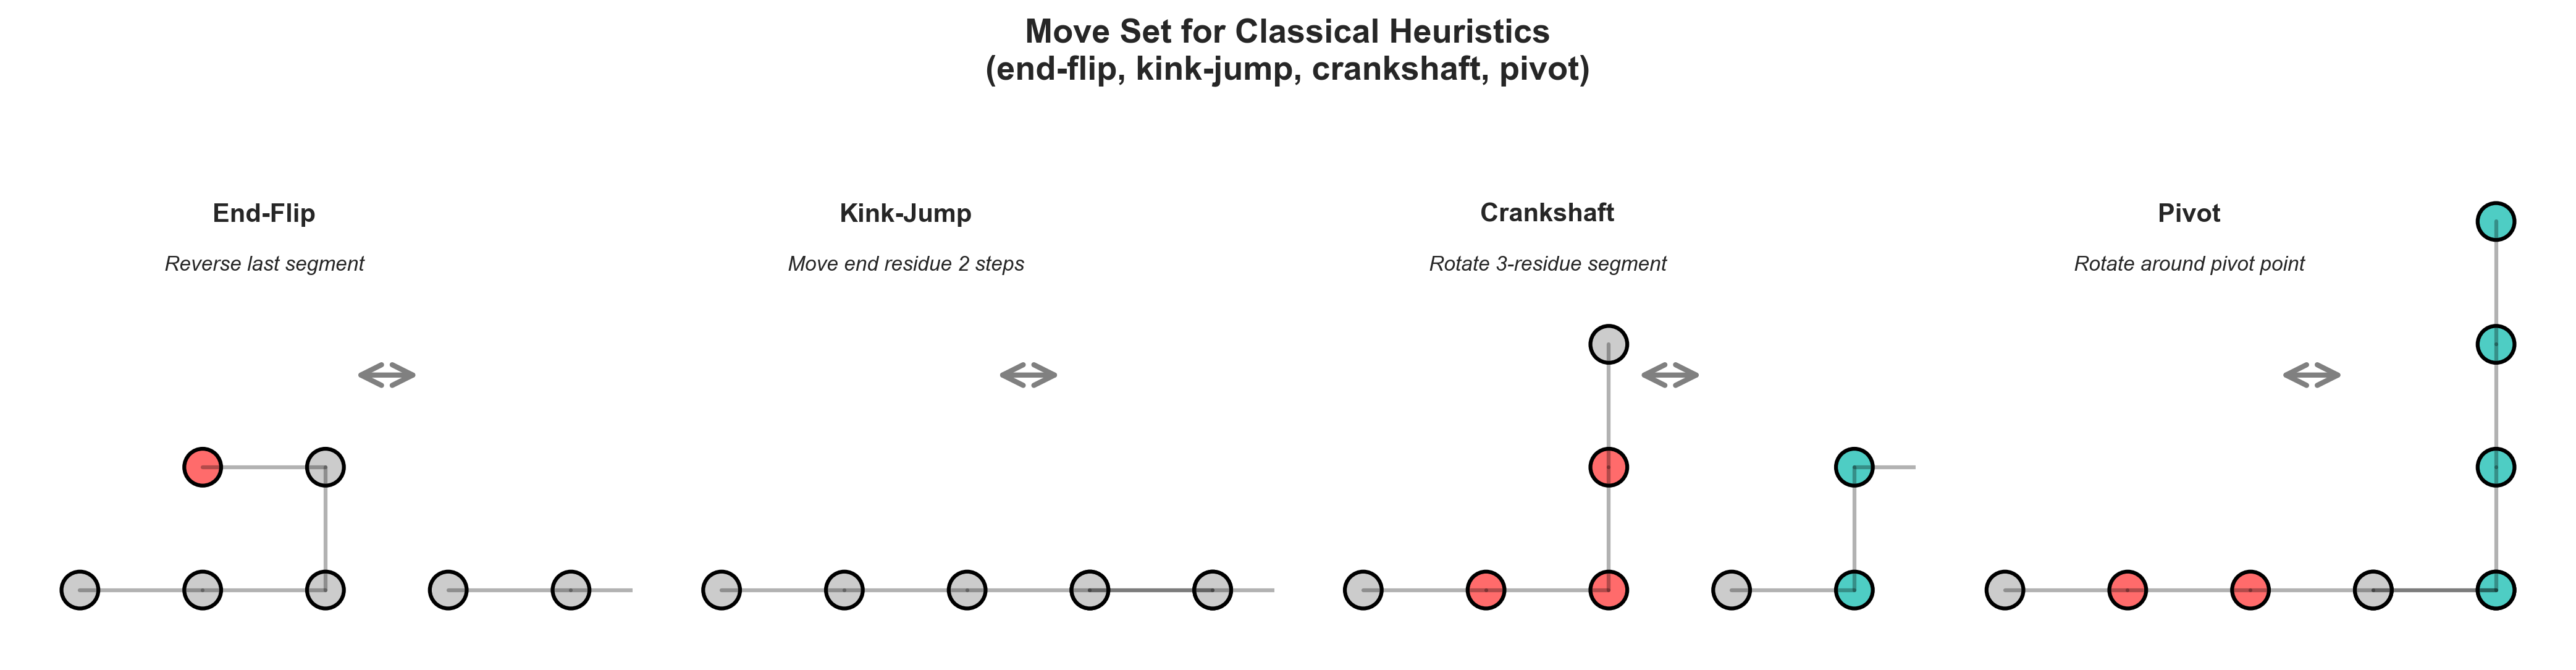
\includegraphics[width=\textwidth]{Figuras/move_set.png}
\caption[Classical heuristic move set]{Move set used by the classical heuristics. The highlighted residues show the part of the chain affected by each local perturbation.}
\label{fig:move_set}
\end{figure}

% ─────────────────────────────────────────────────────────────────────
\section{Classical optimization methods}
\label{cap2:sec_comp_methods}

Because exact enumeration is infeasible, three classical heuristic search algorithms were implemented and benchmarked as baselines.

\subsection{Hill Climbing}
\label{cap2:subsec_hc}

\textbf{Hill Climbing (HC)} is a greedy local search algorithm. Starting from an initial straight-line conformation, it iteratively proposes a random move from the move set and \textbf{accepts it only if the new energy is non-increasing}:
\begin{equation}
    \text{Accept if } E(\mathcal{C}') \leq E(\mathcal{C})
    \label{eq:hc_accept}
\end{equation}
The algorithm maintains a global best solution throughout the search. Although HC is computationally efficient and converges rapidly, it is highly susceptible to \textbf{local minima}: once the algorithm reaches a conformation from which no single move leads to an improvement, the search stalls.

\begin{algorithm}[H]
\caption{Hill Climbing for HP folding}
\label{alg:hc}
\begin{algorithmic}[1]
\State $\mathcal{C} \leftarrow$ straight-line conformation
\State $E_{\text{best}} \leftarrow E(\mathcal{C})$
\For{$t = 1$ \textbf{to} $T_{\max}$}
    \State $m \sim \text{Uniform}(\{\text{end-flip, kink-jump, crankshaft, pivot}\})$
    \State $\mathcal{C}' \leftarrow \text{apply}(m, \mathcal{C})$  \Comment{returns \texttt{None} if invalid}
    \If{$\mathcal{C}' \neq \texttt{None}$ \textbf{and} $E(\mathcal{C}') \leq E(\mathcal{C})$}
        \State $\mathcal{C} \leftarrow \mathcal{C}'$
        \If{$E(\mathcal{C}) < E_{\text{best}}$}
            \State $E_{\text{best}} \leftarrow E(\mathcal{C})$; save best conformation
        \EndIf
    \EndIf
\EndFor
\State \Return best conformation, $E_{\text{best}}$
\end{algorithmic}
\end{algorithm}

\subsection{Simulated Annealing}
\label{cap2:subsec_sa}

\textbf{Simulated Annealing (SA)}, inspired by the metallurgical process of annealing, extends HC by occasionally accepting moves that \textit{worsen} the energy~\cite{kirkpatrick1983optimization}. This probabilistic acceptance criterion allows the search to escape local minima early in the process. The key idea is a temperature parameter $T$ that decreases over time according to a \textbf{cooling schedule}.

A candidate move is accepted with probability:
\begin{equation}
    P(\text{accept}) =
    \begin{cases}
        1 & \text{if } \Delta E \leq 0 \\
        e^{-\Delta E / T} & \text{if } \Delta E > 0
    \end{cases}
    \label{eq:sa_accept}
\end{equation}
where $\Delta E = E(\mathcal{C}') - E(\mathcal{C})$. When the temperature $T$ is high, even largely worse moves are accepted, promoting broad exploration. As $T \rightarrow 0$, the algorithm becomes equivalent to HC.

In this project, an \textbf{exponential cooling schedule} is used:
\begin{equation}
    T_i = T_0 \cdot \left(\frac{T_f}{T_0}\right)^{i / (T_{\max} - 1)}
    \label{eq:sa_cooling}
\end{equation}
where $T_0 = 10.0$ is the initial temperature, $T_f = 0.01$ is the final temperature, and $i$ is the current iteration index.

\begin{algorithm}[H]
\caption{Simulated Annealing for HP folding}
\label{alg:sa}
\begin{algorithmic}[1]
\State $\mathcal{C} \leftarrow$ straight-line conformation; $T \leftarrow T_0$
\For{$t = 1$ \textbf{to} $T_{\max}$}
    \State $T \leftarrow T_0 \cdot (T_f / T_0)^{t/(T_{\max}-1)}$  \Comment{exponential cooling}
    \State $m \sim \text{Uniform}(\text{move set})$; $\mathcal{C}' \leftarrow \text{apply}(m, \mathcal{C})$
    \If{$\mathcal{C}' \neq \texttt{None}$}
        \State $\Delta E \leftarrow E(\mathcal{C}') - E(\mathcal{C})$
        \If{$\Delta E \leq 0$ \textbf{or} $\text{Uniform}(0,1) < e^{-\Delta E / T}$}
            \State $\mathcal{C} \leftarrow \mathcal{C}'$
        \EndIf
        \If{$E(\mathcal{C}) < E_{\text{best}}$}
            \State $E_{\text{best}} \leftarrow E(\mathcal{C})$; save best conformation
        \EndIf
    \EndIf
\EndFor
\State \Return best conformation, $E_{\text{best}}$
\end{algorithmic}
\end{algorithm}

\subsection{Monte Carlo and Replica Exchange Monte Carlo}
\label{cap2:subsec_mc}

\textbf{Monte Carlo (MC)} methods are closely related to SA but operate at a \textit{constant} temperature, using the Metropolis criterion (Equation~\ref{eq:sa_accept}) to accept or reject moves~\cite{metropolis1953equation}. Because the temperature does not change, MC is particularly useful for sampling the thermodynamic ensemble of conformations at a given temperature $T$.

\textbf{Replica Exchange Monte Carlo (REMC)}, also known as parallel tempering, addresses the limitation of single-temperature MC by running $N$ independent MC replicas in parallel, each at a different temperature $T_1 < T_2 < \cdots < T_N$~\cite{hukushima1996exchange,thachuk2007replica}. Periodically, adjacent replicas $k$ and $k+1$ attempt to \textbf{swap} their conformations with probability:
\begin{equation}
    P(\text{swap}) = \min\!\left(1,\; e^{(\beta_k - \beta_{k+1})(E_k - E_{k+1})}\right)
    \label{eq:remc_swap}
\end{equation}
where $\beta_k = 1/T_k$. This exchange mechanism allows low-temperature replicas (which exploit good solutions) to benefit from configurations discovered by high-temperature replicas (which explore broadly), vastly improving the sampling of the energy landscape.

% ─────────────────────────────────────────────────────────────────────
\section{Reinforcement learning}
\label{cap2:sec_rl}

While heuristic algorithms search the energy landscape directly through stochastic perturbations, \textbf{Reinforcement Learning (RL)} approaches the problem differently by training an \textit{agent} to learn \textit{how} to fold a protein through interaction with the environment~\cite{sutton2018reinforcement}.

\subsection{Markov Decision Process formulation}
\label{cap2:subsec_mdp}

The HP folding problem is formulated as a \textbf{Markov Decision Process (MDP)} defined by the tuple $(\mathcal{S}, \mathcal{A}, \mathcal{R}, \mathcal{P}, \gamma)$:

\begin{itemize}
    \item \textbf{State space $\mathcal{S}$:} Each state $s \in \mathcal{S}$ represents the current conformation of the protein chain. In the tabular implementation, this is encoded as a canonical tuple of $(x,y)$ positions, normalized for translation and one rotation symmetry, so that equivalent conformations map to the same state. In the DQN implementation (constructive approach), the state is a rotation-invariant $21 \times 21$ two-channel grid relative to the chain head and current direction.
    \item \textbf{Action space $\mathcal{A}$:} In the classical algorithms (HC, SA, MC, REMC), the agent chooses one of four move types: $\mathcal{A} = \{\text{end-flip},\, \text{kink-jump},\, \text{crankshaft},\, \text{pivot}\}$. In the constructive DQN approach, actions represent relative directions for the next residue: $\mathcal{A} = \{\text{Forward},\, \text{Left},\, \text{Right}\}$, where rotations are applied to the current direction vector.
    \item \textbf{Reward function $\mathcal{R}$:} The reward received after taking action $a$ in state $s$ and transitioning to state $s'$ is:
    \begin{equation}
        R(s, a) =
        \begin{cases}
            E(s) - E(s') & \text{if the move is valid } (= \Delta E > 0 \text{ means energy reduction})\\
            -1 & \text{if the move is invalid (collision / no valid position)}
        \end{cases}
        \label{eq:reward}
    \end{equation}
    This reward is positive when the new conformation has a lower energy (more H-H contacts), zero when energy is unchanged, and negative for invalid moves. The agent therefore learns to prefer energy-reducing moves and to avoid collisions.
    \item \textbf{Discount factor $\gamma \in [0,1)$:} Controls how much the agent values future rewards relative to immediate ones. The tabular implementation used $\gamma = 0.95$, while the DQN training run used $\gamma = 0.99$.
\end{itemize}

\subsection{Tabular Q-Learning}
\label{cap2:subsec_qlearning}

\textbf{Tabular Q-Learning} is a model-free, off-policy RL algorithm~\cite{watkins1992qlearning}. The agent maintains a table (the \textit{Q-table}) $Q: \mathcal{S} \times \mathcal{A} \rightarrow \mathbb{R}$, where $Q(s, a)$ represents the expected cumulative discounted reward obtained by taking action $a$ in state $s$ and then following the optimal policy. Q-values are updated iteratively using the \textbf{Bellman equation}:

\begin{equation}
    Q(s,a) \leftarrow Q(s,a) + \alpha \left[ R(s,a) + \gamma \max_{a'} Q(s',a') - Q(s,a) \right]
    \label{eq:qlearning}
\end{equation}

where $\alpha \in (0,1]$ is the \textit{learning rate} (set to $0.1$) that controls how quickly new information overrides old estimates, and $\gamma = 0.95$ is the discount factor. The term $R(s,a) + \gamma \max_{a'} Q(s',a')$ is called the \textit{TD target} (Temporal Difference target), and $\delta = \text{TD target} - Q(s,a)$ is the \textit{TD error}.

Action selection follows an \textbf{$\varepsilon$-greedy policy}: with probability $\varepsilon$ the agent selects a random action (exploration), and with probability $1 - \varepsilon$ it selects the action with the highest Q-value (exploitation). The exploration rate $\varepsilon$ is decayed linearly from $1.0$ to $0.05$ over the first half of training:

\begin{equation}
    \varepsilon_t = \max\!\left(\varepsilon_{\min},\; \varepsilon_0 - (\varepsilon_0 - \varepsilon_{\min}) \cdot \frac{t}{\lfloor T_{\text{decay}} \rfloor}\right)
    \label{eq:epsilon_decay}
\end{equation}

where $T_{\text{decay}} = \lfloor \text{episodes} \times \text{steps\_per\_episode} / 2 \rfloor$.

\begin{algorithm}[H]
\caption{Tabular Q-Learning for HP folding}
\label{alg:ql}
\begin{algorithmic}[1]
\State Initialize $Q(s,a) \leftarrow 0$ for all $s, a$; $\varepsilon \leftarrow 1.0$
\For{each episode}
    \State $\mathcal{C} \leftarrow$ straight-line conformation; $s \leftarrow \text{encode}(\mathcal{C})$
    \For{each step}
        \State Decay $\varepsilon$ according to Equation~\ref{eq:epsilon_decay}
        \If{$\text{Uniform}(0,1) < \varepsilon$}
            \State $a \leftarrow \text{random action}$ \Comment{explore}
        \Else
            \State $a \leftarrow \arg\max_{a'} Q(s, a')$ \Comment{exploit}
        \EndIf
        \State $\mathcal{C}' \leftarrow \text{apply}(a, \mathcal{C})$
        \State Compute reward $R$ via Equation~\ref{eq:reward}
        \State $s' \leftarrow \text{encode}(\mathcal{C}')$
        \State $Q(s,a) \leftarrow Q(s,a) + \alpha[R + \gamma \max_{a''} Q(s',a'') - Q(s,a)]$
        \State $s \leftarrow s'$; $\mathcal{C} \leftarrow \mathcal{C}'$; update global best
    \EndFor
\EndFor
\State \Return best conformation, $E_{\text{best}}$, $Q$-table
\end{algorithmic}
\end{algorithm}

Tabular Q-Learning is effective for short sequences (up to $\approx 25$ residues) but suffers from the \textit{curse of dimensionality}: the number of distinct conformations grows exponentially with chain length, making the Q-table intractably large for realistic proteins.

% ─────────────────────────────────────────────────────────────────────
\section{Deep reinforcement learning}
\label{cap2:sec_drl}

\textbf{Deep Reinforcement Learning (DRL)} overcomes the scalability limitation by replacing the Q-table with a parametric function approximator: a \textbf{Deep Q-Network (DQN)} introduced by Mnih et al.~\cite{mnih2015human}. Instead of storing one Q-value per state-action pair, the network $Q(s, a; \theta)$ with parameters $\theta$ maps a state representation directly to a vector of Q-values for all actions.

\subsection{State representation}
\label{cap2:subsec_state_rep}

In the constructive DQN implementation, the state is encoded as a two-channel grid of size $21 \times 21$ (nine times smaller, focusing only on the local neighborhood). The encoding is rotation-invariant: the grid is centered on the chain's head (last positioned residue) and rotated so that the current direction vector always points upward. Each channel encodes residue type:
\begin{equation}
    g_{\text{channel}}[x, y] =
    \begin{cases}
        1.0 & \text{if a residue of the corresponding type occupies the rotated position } (x, y) \\
        0.0  & \text{(empty site)}
    \end{cases}
    \label{eq:grid_encoding_new}
\end{equation}
Channel 0 represents Hydrophobic (H) residues, channel 1 represents Polar (P) residues. This rotation-invariant encoding dramatically reduces state space size while ensuring that the CNN learns folding patterns that are independent of the chain's global position and orientation, enabling better generalization across proteins of different lengths and H-content.

\subsection{Network architecture}
\label{cap2:subsec_cnn}

The neural network is a \textbf{Convolutional Neural Network (CNN)} designed to process $2 \times 21 \times 21$ inputs. The final architecture used in the Colab-trained model consists of:

\begin{enumerate}
    \item \textbf{Input:} Two-channel grid ($2 \times 21 \times 21$) representing H and P residue positions.
    \item \textbf{Convolutional block 1:} \texttt{Conv2d}($2, 32$, kernel $3\times3$, padding $1$) $\rightarrow$ \texttt{ReLU}. Output: $32 \times 21 \times 21$.
    \item \textbf{Convolutional block 2:} \texttt{Conv2d}($32, 64$, kernel $3\times3$, padding $1$) $\rightarrow$ \texttt{ReLU}. Output: $64 \times 21 \times 21$.
    \item \textbf{Convolutional block 3:} \texttt{Conv2d}($64, 64$, kernel $3\times3$, padding $1$) $\rightarrow$ \texttt{ReLU}. Output: $64 \times 21 \times 21$.
    \item \textbf{Flatten:} $64 \times 21 \times 21 = 28{,}224$ features.
    \item \textbf{Fully connected:} \texttt{Linear}($28224, 256$) $\rightarrow$ \texttt{ReLU} $\rightarrow$ \texttt{Linear}($256, 3$).
\end{enumerate}

The output layer produces 3 Q-values, one per relative direction action (Forward, Left, Right). The compact $21 \times 21$ grid dramatically reduces memory overhead while focusing on local patterns. Combined with the rotation-invariant encoding, this architecture enables the CNN to learn generalizable folding strategies that transfer effectively across proteins of different lengths and compositions.

\begin{figure}[htbp]
\centering
\small
\setlength{\tabcolsep}{3pt}
\resizebox{\textwidth}{!}{%
\begin{tabular}{ccccccccccccc}
\fcolorbox{black}{blue!10}{\parbox[c][2.3cm][c]{2.5cm}{\centering
\textbf{Input State}\\
$2 \times 21 \times 21$\\
H/P channels\\
\footnotesize rotation-invariant grid}}
& $\rightarrow$ &
\fcolorbox{black}{green!12}{\parbox[c][2.3cm][c]{2.5cm}{\centering
\textbf{Conv2D + ReLU}\\
$2 \rightarrow 32$\\
$3 \times 3$, padding 1\\
\footnotesize $32 \times 21 \times 21$}}
& $\rightarrow$ &
\fcolorbox{black}{green!12}{\parbox[c][2.3cm][c]{2.5cm}{\centering
\textbf{Conv2D + ReLU}\\
$32 \rightarrow 64$\\
$3 \times 3$, padding 1\\
\footnotesize $64 \times 21 \times 21$}}
& $\rightarrow$ &
\fcolorbox{black}{green!12}{\parbox[c][2.3cm][c]{2.5cm}{\centering
\textbf{Conv2D + ReLU}\\
$64 \rightarrow 64$\\
$3 \times 3$, padding 1\\
\footnotesize $64 \times 21 \times 21$}}
& $\rightarrow$ &
\fcolorbox{black}{yellow!20}{\parbox[c][2.3cm][c]{2.0cm}{\centering
\textbf{Flatten}\\
28,224\\
features}}
& $\rightarrow$ &
\fcolorbox{black}{orange!15}{\parbox[c][2.3cm][c]{2.0cm}{\centering
\textbf{FC + ReLU}\\
$28{,}224 \rightarrow 256$}}
& $\rightarrow$ &
\fcolorbox{black}{red!12}{\parbox[c][2.3cm][c]{1.8cm}{\centering
\textbf{Output}\\
$256 \rightarrow 3$\\
Q-values\\
\footnotesize F/L/R}}
\end{tabular}%
}

\vspace{0.6em}

\resizebox{0.9\textwidth}{!}{%
\begin{tabular}{cccc}
\fcolorbox{black}{gray!12}{\parbox[c][1.15cm][c]{3.0cm}{\centering
\textbf{Replay Buffer}\\
100,000 transitions}}
&
\fcolorbox{black}{gray!12}{\parbox[c][1.15cm][c]{3.2cm}{\centering
\textbf{Target Network}\\
sync every 1,000 optimization steps}}
&
\fcolorbox{black}{gray!12}{\parbox[c][1.15cm][c]{3.0cm}{\centering
\textbf{Exploration}\\
$\varepsilon$: $1.0 \rightarrow 0.05$}}
&
\fcolorbox{black}{gray!12}{\parbox[c][1.15cm][c]{3.0cm}{\centering
\textbf{Stabilization}\\
Double DQN + clipping 10}}
\end{tabular}%
}
\caption[Constructive DQN architecture]{Constructive DQN architecture used for residue-by-residue folding. The two input channels encode hydrophobic and polar residues, and the output layer estimates Q-values for the relative actions Forward, Left and Right.}
\label{fig:dqn_architecture}
\end{figure}

\subsection{Training procedure}
\label{cap2:subsec_dqn_training}

DQN training relies on key stabilization mechanisms:

\begin{itemize}
    \item \textbf{Constructive Environment:} Unlike perturbative approaches that start with a straight line and modify it, the constructive environment builds the protein one amino acid at a time. The first two residues are positioned to define an initial direction; subsequent residues are placed via relative direction decisions (Forward/ Left/ Right). This guarantees self-avoiding walks by design and simplifies the state space.
    \item \textbf{Experience Replay:} Transitions $(s, a, r, s')$ are stored in a \textit{Replay Buffer} of capacity $100{,}000$. At each training step, a random mini-batch (batch size 128) is sampled. This breaks temporal correlations and reduces gradient variance.
    \item \textbf{Target Network:} A separate network copy, $Q(s, a; \theta^-)$, computes TD targets. Its weights $\theta^-$ are synchronized every 1,000 optimization steps, preventing oscillations from constantly moving targets.
    \item \textbf{Reward Structure:} $R = +1.0$ for each new H-H contact formed (direct energy feedback), $-1.0$ for invalid moves (collisions), $+0.5$ bonus for completing the full chain without collision, with additional shaping for low-H-density proteins.
    \item \textbf{Stability Mechanisms:} The training loop uses Double DQN target selection and gradient clipping with maximum norm 10.
\end{itemize}

The loss function is the \textbf{Mean Squared Error (MSE)} between predicted and target Q-values. In the final implementation, the target action is selected by the policy network and evaluated by the target network, following the Double DQN formulation:
\begin{equation}
    a^* = \arg\max_{a'} Q(s', a'; \theta)
    \quad ; \quad
    y = r + \gamma Q(s', a^*; \theta^-)(1-done)
    \quad ; \quad
    \mathcal{L}(\theta) = \mathbb{E}_{(s,a,r,s') \sim \mathcal{D}} \left[ \left( y - Q(s, a; \theta) \right)^2 \right]
    \label{eq:dqn_loss}
\end{equation}
Network parameters $\theta$ are optimized via \textbf{Adam}~\cite{kingma2015adam} with learning rate $\eta = 0.001$, $\gamma = 0.99$, and $\varepsilon$-decay from 1.0 to 0.05 over training. Training is performed on a dataset of 20 real UniProt proteins for 20,000 episodes, with GPU acceleration available.

\begin{algorithm}[H]
\caption{Constructive Deep Q-Network for HP folding}
\label{alg:dqn_constructive}
\begin{algorithmic}[1]
\State Initialize policy network $Q(s,a;\theta)$ and target network $Q(s,a;\theta^-)$
\State Copy initial weights: $\theta^- \leftarrow \theta$
\State Initialize replay buffer $\mathcal{D}$ with capacity $100{,}000$
\State Set $\varepsilon \leftarrow 1.0$, $\varepsilon_{\min} \leftarrow 0.05$, $\gamma \leftarrow 0.99$
\For{episode $= 1$ to $20{,}000$}
    \State Sample one HP sequence from the training set
    \State Reset constructive environment with first two residues fixed
    \While{the chain is not complete and no collision occurred}
        \State Encode partial chain as a $2 \times 21 \times 21$ rotation-invariant grid $s$
        \If{$\mathrm{Uniform}(0,1) < \varepsilon$}
            \State Select random action $a \in \{\text{Forward}, \text{Left}, \text{Right}\}$
        \Else
            \State Select $a = \arg\max_{a'} Q(s,a';\theta)$
        \EndIf
        \State Apply $a$ to place the next residue and observe $(r, s', done)$
        \State Store transition $(s,a,r,s',done)$ in $\mathcal{D}$
        \If{$|\mathcal{D}|$ is larger than the mini-batch size}
            \State Sample a random mini-batch from $\mathcal{D}$
            \State Select $a^* = \arg\max_{a'} Q(s',a';\theta)$ and compute $y = r + \gamma Q(s',a^*;\theta^-)(1-done)$
            \State Update $\theta$ by minimizing $\left(y - Q(s,a;\theta)\right)^2$
        \EndIf
    \EndWhile
    \State Decay $\varepsilon \leftarrow \max(\varepsilon_{\min}, 0.995\varepsilon)$
    \If{1,000 optimization steps have elapsed}
        \State Synchronize target network: $\theta^- \leftarrow \theta$
    \EndIf
\EndFor
\State Save trained weights to \texttt{dqn\_weights.pth}
\end{algorithmic}
\end{algorithm}

% ─────────────────────────────────────────────────────────────────────
\section{Summary}
\label{cap2:sec_summary}

This chapter detailed the theoretical concepts underlying the computational approaches to the 2D protein folding problem. We began by formalizing the HP lattice model, defining the notion of topological neighbours and the HP energy function. We then described the shared move set (end-flip, kink-jump, crankshaft, pivot) used by all algorithms. For the classical baseline methods, each algorithm was presented individually: Hill Climbing as a fast but locally trapped greedy search, Simulated Annealing as a temperature-controlled stochastic method capable of escaping local minima, and Replica Exchange Monte Carlo as a parallel, multi-temperature approach for robust landscape exploration. Finally, we introduced the Reinforcement Learning paradigm, formally defining the MDP formulation including the state space, action space, and reward function. We traced the evolution from Tabular Q-Learning which learns discrete folding policies via the Bellman equation and $\varepsilon$-greedy exploration to Deep Q-Networks, which replace the Q-table with a CNN capable of processing large spatial grids, offering a scalable method for predicting the structures of complex proteins.


% Capítulo 3
\chapter{Web platform}
\label{cap3}

This chapter details the design, development, and testing of the interactive web platform created for this project. The platform serves as the primary user-facing interface, enabling seamless protein sequence analysis, functional annotation via external deep learning APIs, and 2D structure visualization through locally implemented optimization algorithms. The chapter outlines the system requirements, describes the interface prototype, explains the technical implementation and architecture, and discusses the testing procedures employed to ensure reliability and correctness.

% ─────────────────────────────────────────────────────────────────────
\section{Requirement analysis}
\label{cap3:sec_requirements}

To provide a robust and accessible tool for computational biology, the web platform was designed to meet the following functional and non-functional requirements:

\begin{itemize}
    \item \textbf{Sequence Input Processing:} The system must accept protein sequences in standard FASTA format, capable of parsing multiple sequences simultaneously. A dedicated utility function strips FASTA headers (lines beginning with \texttt{>}) and validates that only legal amino acid characters are processed.

    \item \textbf{Function Prediction Integration:} The platform must seamlessly integrate with the external \textbf{DeepGO} API~\cite{kulmanov2018deepgo} to retrieve and display Gene Ontology (GO) terms categorized into three domains: Biological Process (GO:BP), Molecular Function (GO:MF), and Cellular Component (GO:CC).

    \item \textbf{Algorithm Selection and Configuration:} Users must be able to select from a suite of 2D structure prediction algorithms Hill Climbing (HC), Simulated Annealing (SA), Monte Carlo (MC), Replica Exchange Monte Carlo (REMC), and the trained Deep Q-Network (DQN) and configure their respective hyperparameters (e.g., number of iterations, temperature range, number of replicas, number of DQN rollouts, and visualization step interval). The final interface configuration is illustrated in Appendix~A.

    \item \textbf{Structure Visualization:} The platform must generate a visual SVG-based representation of the folded protein on a 2D HP lattice, accurately depicting Hydrophobic (H) and Polar (P) amino acids with distinct colors, rendering the backbone chain, and reporting the total computed energy.

    \item \textbf{3D Structure Retrieval:} As an extended feature, the system should act as a bridge to fetch known or predicted 3D structures from the \textbf{AlphaFold DB}~\cite{varadi2022alphafold} and the \textbf{ESMFold API}~\cite{lin2023evolutionary}, returning PDB-format files for further visualization.

    \item \textbf{Responsiveness and Usability:} The interface must be responsive across different screen sizes and provide clear, user-friendly error messages for invalid inputs, API failures, or algorithm errors.
\end{itemize}

% ─────────────────────────────────────────────────────────────────────
\section{User prototype}
\label{cap3:sec_prototype}

The user interface was prototyped with a focus on simplicity, clarity, and ease of use for researchers and students unfamiliar with command-line tools. The layout is divided into the following sections:

\begin{itemize}
    \item \textbf{Input Interface:} A prominent text area allows users to paste raw FASTA sequences. A set of radio buttons and dropdown menus positioned below the input box allow the user to select the desired action (\textit{Predict GO Terms} or \textit{Generate 2D Structure}) and choose a specific optimization algorithm.

    \item \textbf{Hyperparameter Panel:} When the \textit{Structure} action is selected, context-sensitive input fields appear dynamically, allowing experienced users to fine-tune algorithm parameters. For example: number of iterations for HC/SA/MC, number of replicas and temperature range for REMC, number of DQN rollouts, and the interval at which intermediate folding steps should be displayed.

    \item \textbf{Results Dashboard:} The output is presented in a structured panel. For function prediction, GO terms are displayed in categorized, expandable lists with their associated confidence scores. For structure prediction, the interface renders the 2D lattice graphically using an auto-scaling SVG canvas, highlighting H residues (colored) and P residues (distinct color), drawing the backbone chain, and displaying the computed minimum energy. A step explorer allows users to inspect intermediate conformations every user-defined number of iterations; for DQN, this corresponds to the constructive residue-by-residue folding trajectory. Appendix~B shows representative screenshots of this step-by-step visualization from the initial partial chain to the final conformation.

    \item \textbf{3D Viewer Integration:} A dedicated section allows users to enter a UniProt accession code and fetch the corresponding 3D structure from AlphaFold DB or ESMFold, displaying or providing a download link to the resulting PDB file.
\end{itemize}

% ─────────────────────────────────────────────────────────────────────
\section{Implementation}
\label{cap3:sec_implementation}

The web platform was implemented using \textbf{Django 6.0.2}, a high-level Python web framework that encourages rapid development and clean, pragmatic design~\cite{django2024}. The overall system follows a \textbf{Model-View-Template (MVT)} architecture.

\begin{figure}[htbp]
\centering
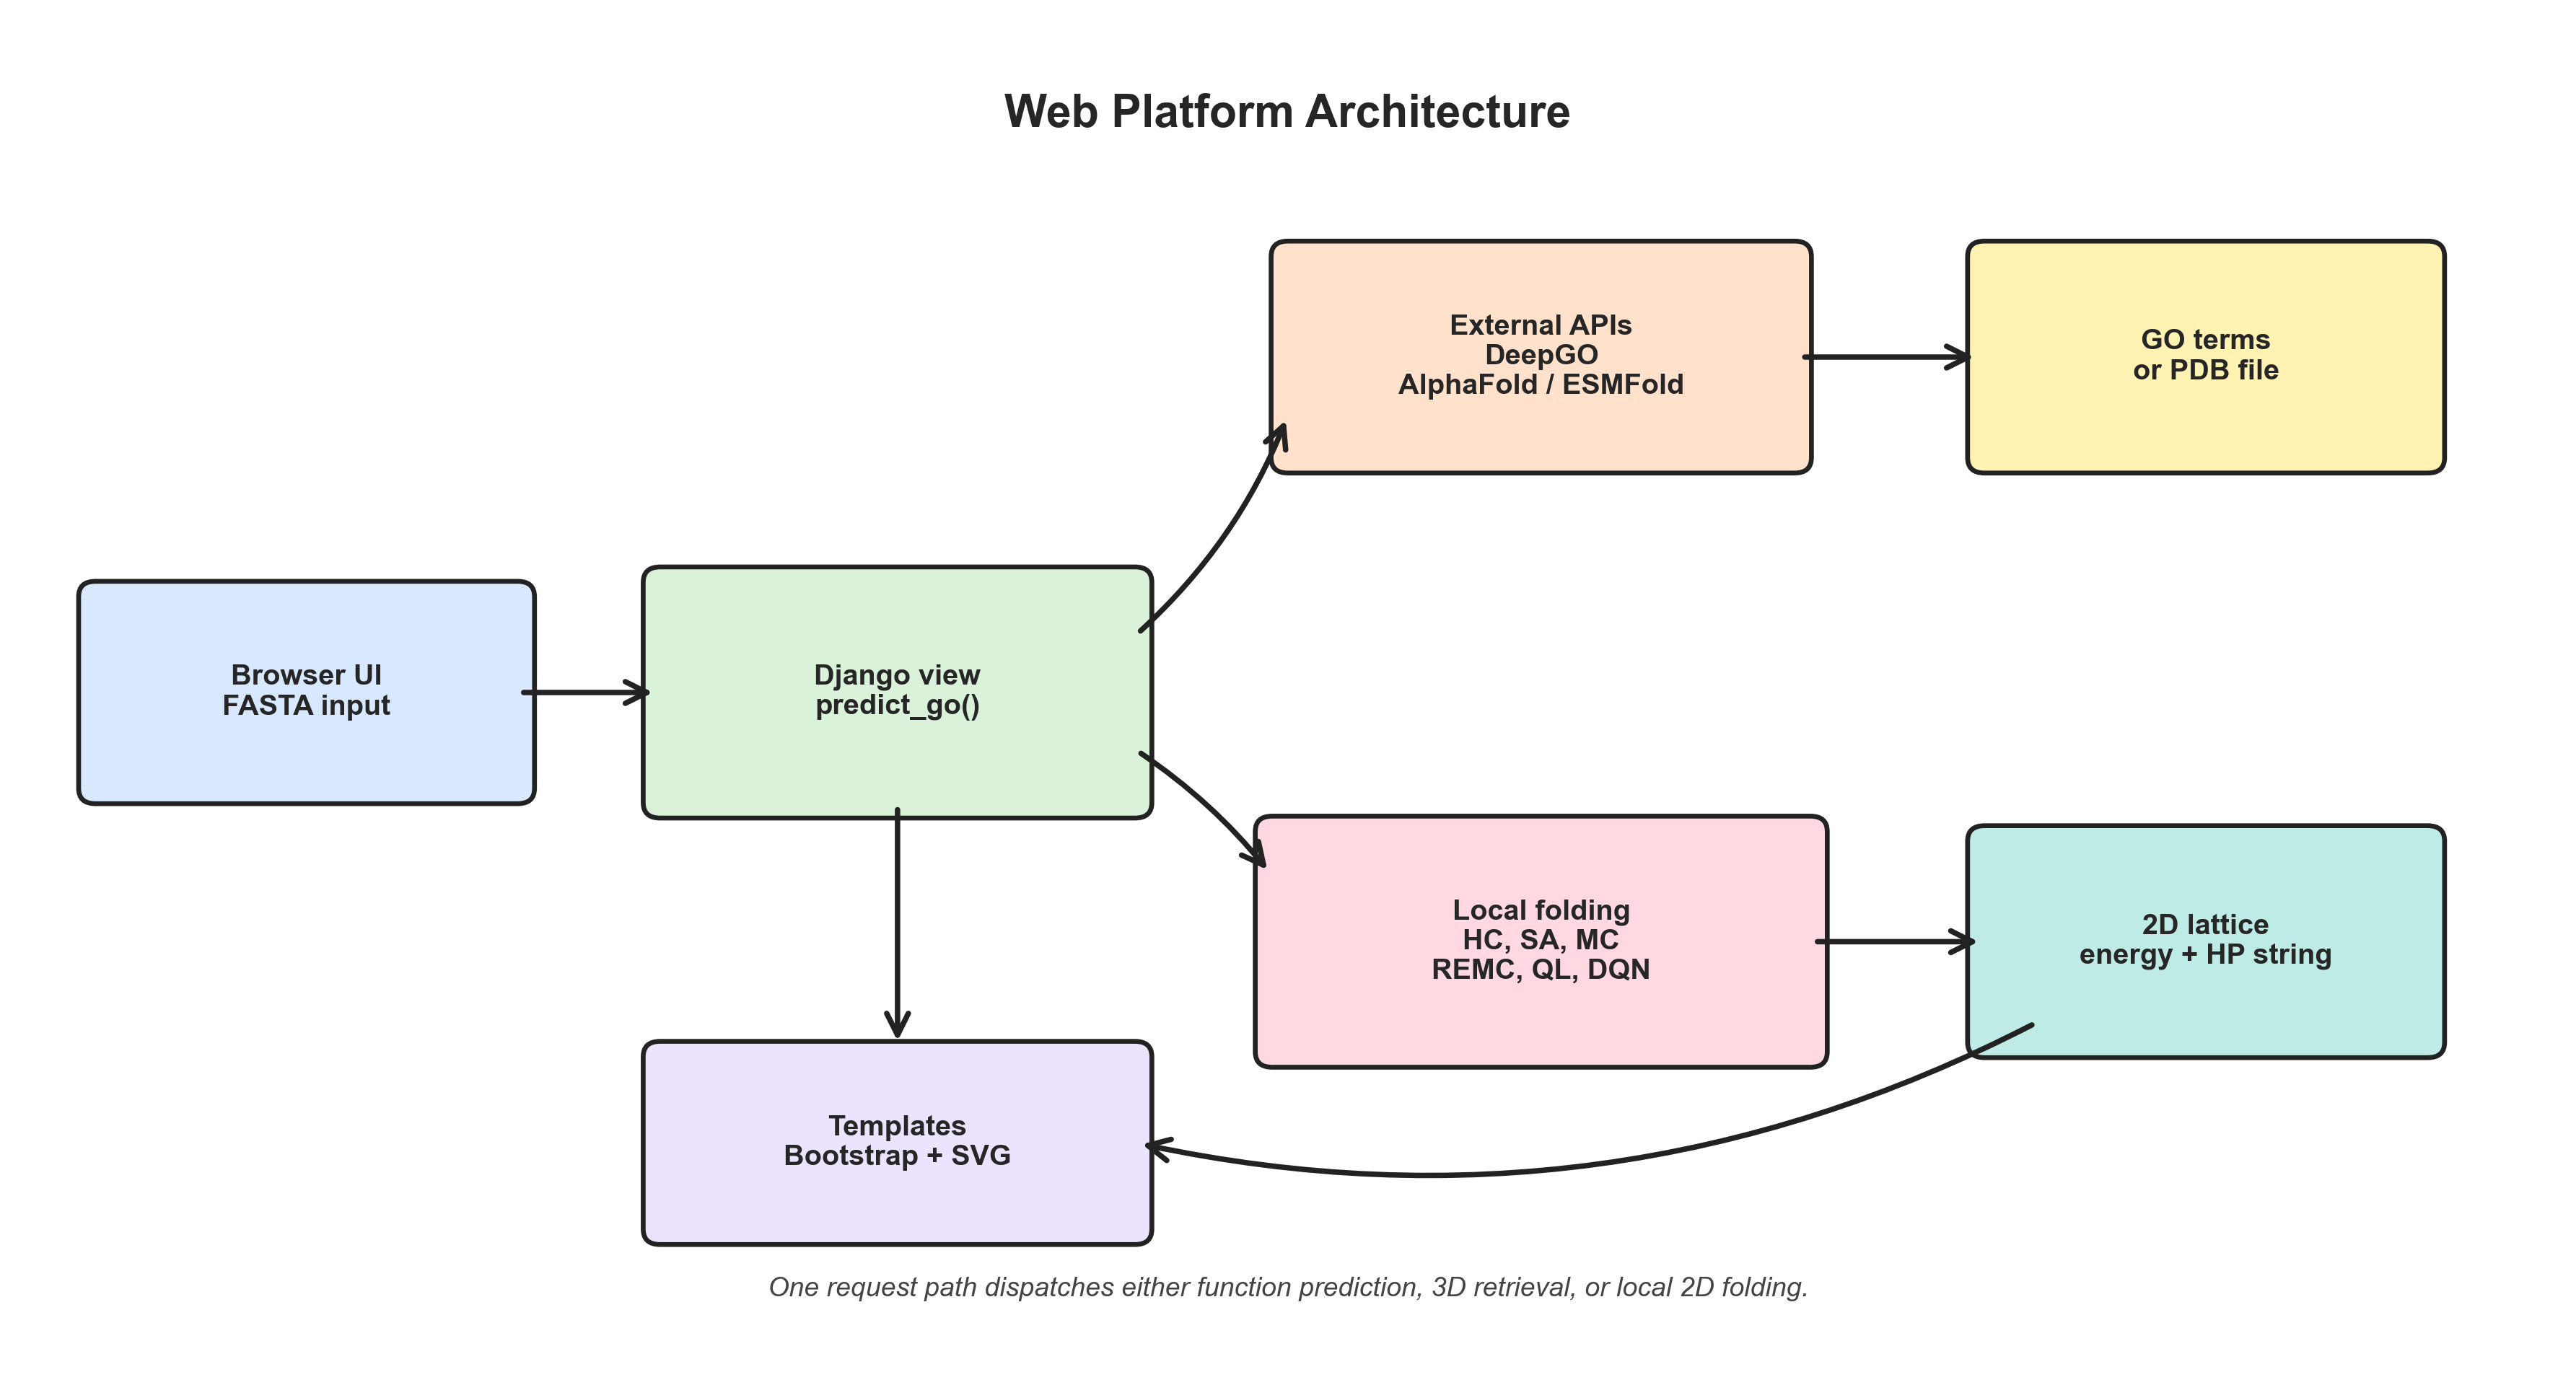
\includegraphics[width=\textwidth]{Figuras/web_platform_architecture.png}
\caption[Web platform architecture]{High-level architecture of the web platform. A single Django view dispatches requests to either external services for function/3D prediction or local HP-folding algorithms for 2D structure generation.}
\label{fig:web_platform_architecture}
\end{figure}

\subsection{Backend architecture}
\label{cap3:subsec_backend}

The core logic resides in \texttt{go\_predictor/views.py}, which acts as the controller:

\begin{itemize}
    \item \textbf{Request routing:} The main view function receives \texttt{POST} requests containing the FASTA sequence, the selected action, and hyperparameter values. It dispatches processing to the appropriate function based on the action type.
    \item \textbf{FASTA parsing:} A utility function strips header lines and concatenates residue characters, performing basic validation (only A--Z characters representing amino acids are accepted).
    \item \textbf{HP translation:} The raw amino acid sequence is converted to a binary HP string using a fixed hydrophobic residue set (\texttt{ACFILMVWY}), following the standard HP model classification.
\end{itemize}

\subsection{Algorithmic integration}
\label{cap3:subsec_algo_integration}

The web application dynamically imports the production structure prediction scripts located in the project's \texttt{tests/} directory and the trained DQN inference module. This modular architecture decouples the web interface from the computational logic:

\begin{itemize}
    \item \texttt{test\_hc.py} --- Hill Climbing (\texttt{generate\_2d\_structure})
    \item \texttt{test\_sa.py} --- Simulated Annealing (\texttt{generate\_2d\_structure\_sa})
    \item \texttt{test\_mc.py} --- Monte Carlo (\texttt{generate\_2d\_structure\_mc})
    \item \texttt{test\_remc.py} --- Replica Exchange Monte Carlo (\texttt{generate\_2d\_structure\_remc})
    \item \texttt{agent\_dqn\_model.py} --- Constructive DQN inference (\texttt{run\_dqn\_inference})
\end{itemize}

Each function returns a list of $(x, y)$ lattice coordinates and the best energy found. For interactive visualization, the classical algorithms can optionally return trace frames at a user-defined interval, while the constructive DQN returns residue-placement frames. The view passes these coordinates to the SVG renderer, which maps them to pixel positions on an auto-scaling canvas. The Tabular Q-Learning implementation remains available in \texttt{test\_ql.py} for offline benchmarking, but it is not imported by the production web view because the trained DQN replaces it for real-time inference.

\subsection{External API communication}
\label{cap3:subsec_api}

The \texttt{requests} library is used to communicate with external services:

\begin{itemize}
    \item \textbf{DeepGO API:} The \texttt{call\_deepgo\_api} function packages the user's sequence into a JSON payload and sends a \texttt{POST} request to the DeepGO inference endpoint. The returned JSON containing GO term identifiers and confidence scores for all three ontology domains is parsed and structured for display in the template.
    \item \textbf{AlphaFold DB:} A \texttt{GET} request is sent to the AlphaFold prediction API using the UniProt accession as query input. This retrieves the metadata associated with the specified protein. The application then extracts the \texttt{pdbUrl} field returned by the API and uses it to download or render the corresponding PDB file. This avoids hard-coding a specific AlphaFold file-version suffix such as \texttt{model\_v4}.
    \item \textbf{ESMFold API:} A \texttt{POST} request to the ESMFold endpoint sends the raw sequence and receives a PDB-format response, allowing users to obtain predicted structures without a local installation.
\end{itemize}

All external calls are wrapped in \texttt{try-except} blocks to handle network timeouts, invalid accession codes, and API rate limits, returning descriptive error messages to the user rather than server faults.

\subsection{Frontend design}
\label{cap3:subsec_frontend}

The frontend is built with \textbf{HTML5}, \textbf{CSS3}, \textbf{Tailwind CSS}, and Lucide icons to ensure a responsive and visually consistent layout. Django's template engine is used to dynamically inject algorithmic results, loop over GO term lists, and conditionally show/hide interface sections based on the selected action. The SVG 2D structure visualization is embedded directly into the response HTML and updated client-side by JavaScript when the user moves the step slider.

% ─────────────────────────────────────────────────────────────────────
\section{Tests}
\label{cap3:sec_tests}

Rigorous testing was conducted to ensure the platform's stability, accuracy, and robustness:

\begin{itemize}
    \item \textbf{Integration Testing:} The Django backend was verified to correctly invoke the standalone algorithmic scripts with the parameters provided by the user interface. Edge cases were tested: sequences of length 1 (single residue), sequences composed entirely of 'P' residues (zero H-H contacts, energy $= 0$), and very long sequences ($> 100$ residues) to verify graceful degradation.

    \item \textbf{FASTA Validation:} The parser was tested against malformed inputs missing headers, sequences with non-amino-acid characters, empty submissions, and mixed-case inputs confirming that invalid data is rejected with user-friendly error messages before reaching the computational modules.

    \item \textbf{API Reliability:} Connections to DeepGO, AlphaFold, and ESMFold were tested under simulated failure conditions (invalid accession codes, network unavailability). Exception handling confirmed that the server returns descriptive error messages rather than \texttt{500 Internal Server Error} responses.

    \item \textbf{Visualization Correctness:} The SVG renderer was validated by comparing the rendered structures against manually computed expected positions for small sequences (up to 10 residues), verifying that backbone links connect consecutive residues and that H/P color assignments are consistent with the HP string.

    \item \textbf{Hyperparameter Passthrough:} It was verified that user-specified hyperparameter values (e.g., \texttt{iterations=50000}, temperature values, replica counts, DQN rollouts, and step-visualization intervals) are correctly parsed from the form POST data, validated to be in acceptable ranges, and passed to the underlying algorithm functions.
\end{itemize}

% ─────────────────────────────────────────────────────────────────────
\section{Summary}
\label{cap3:sec_summary}

This chapter described the design and implementation of the web platform that serves as the user-facing component of the project. The requirement analysis guided the development of a functional interface prototype, which was implemented using Django's MVT architecture, cleanly separating web request handling from the computationally intensive algorithmic logic. The modular algorithmic integration allows the implemented algorithms (HC, SA, MC, REMC and DQN) to be invoked through a unified interface. External API communication with DeepGO, AlphaFold, and ESMFold was robustly handled with appropriate error management. Comprehensive testing confirmed that the platform correctly handles user inputs, algorithm execution, step visualization, and external API interactions across a range of normal and edge-case scenarios.


% Chapter 4
\chapter{Algorithm development}
\label{cap4}

This chapter focuses on the practical implementation of the computational methods used to solve the 2D HP protein folding problem. It describes the full prediction pipeline from raw sequence to lattice coordinates, details the specific implementation of each algorithm, and presents a quantitative comparative analysis of their performance on a benchmark dataset of 20 real UniProt protein sequences.

% ─────────────────────────────────────────────────────────────────────
\section{Protein 2D structure prediction pipeline}
\label{cap4:sec_pipeline}

The structure prediction pipeline processes a raw amino acid sequence through the following stages:

\begin{enumerate}
    \item \textbf{HP Translation:} The input sequence is scanned character by character. Each amino acid is classified as Hydrophobic (H) if it belongs to the set \texttt{\{A, C, F, I, L, M, V, W, Y\}} or Polar (P) otherwise, producing a binary HP string of the same length.

    \item \textbf{Initialization:} The protein is initialized as a straight horizontal line: residue $i$ is placed at position $(i, 0)$. This is always a valid self-avoiding walk (SAW) and provides a neutral, unbiased starting conformation with energy 0 (no H-H contacts in a straight line unless residues happen to be placed adjacently by the walk).

    \item \textbf{Energy Evaluation:} At each step, the conformation is evaluated using the HP energy function defined in Equation~\ref{eq:hp_energy}. In the implementation, this is computed by building a dictionary \texttt{\{(x,y): index\}} from the current positions, then for each H residue iterating over its four Manhattan neighbours and counting non-consecutive H-H contacts. The result is divided by 2 (since each contact is counted twice) and negated to give a negative energy.

    \item \textbf{Optimization:} The chosen algorithm iteratively modifies the conformation using the shared move set (end-flip, kink-jump, crankshaft, pivot) and its specific acceptance criterion.

    \item \textbf{Output:} The algorithm returns the best conformation found (as a list of $(x, y)$ coordinates), the corresponding minimum energy, and any learned parameters (Q-table or neural network weights).
\end{enumerate}

\begin{figure}[htbp]
\centering
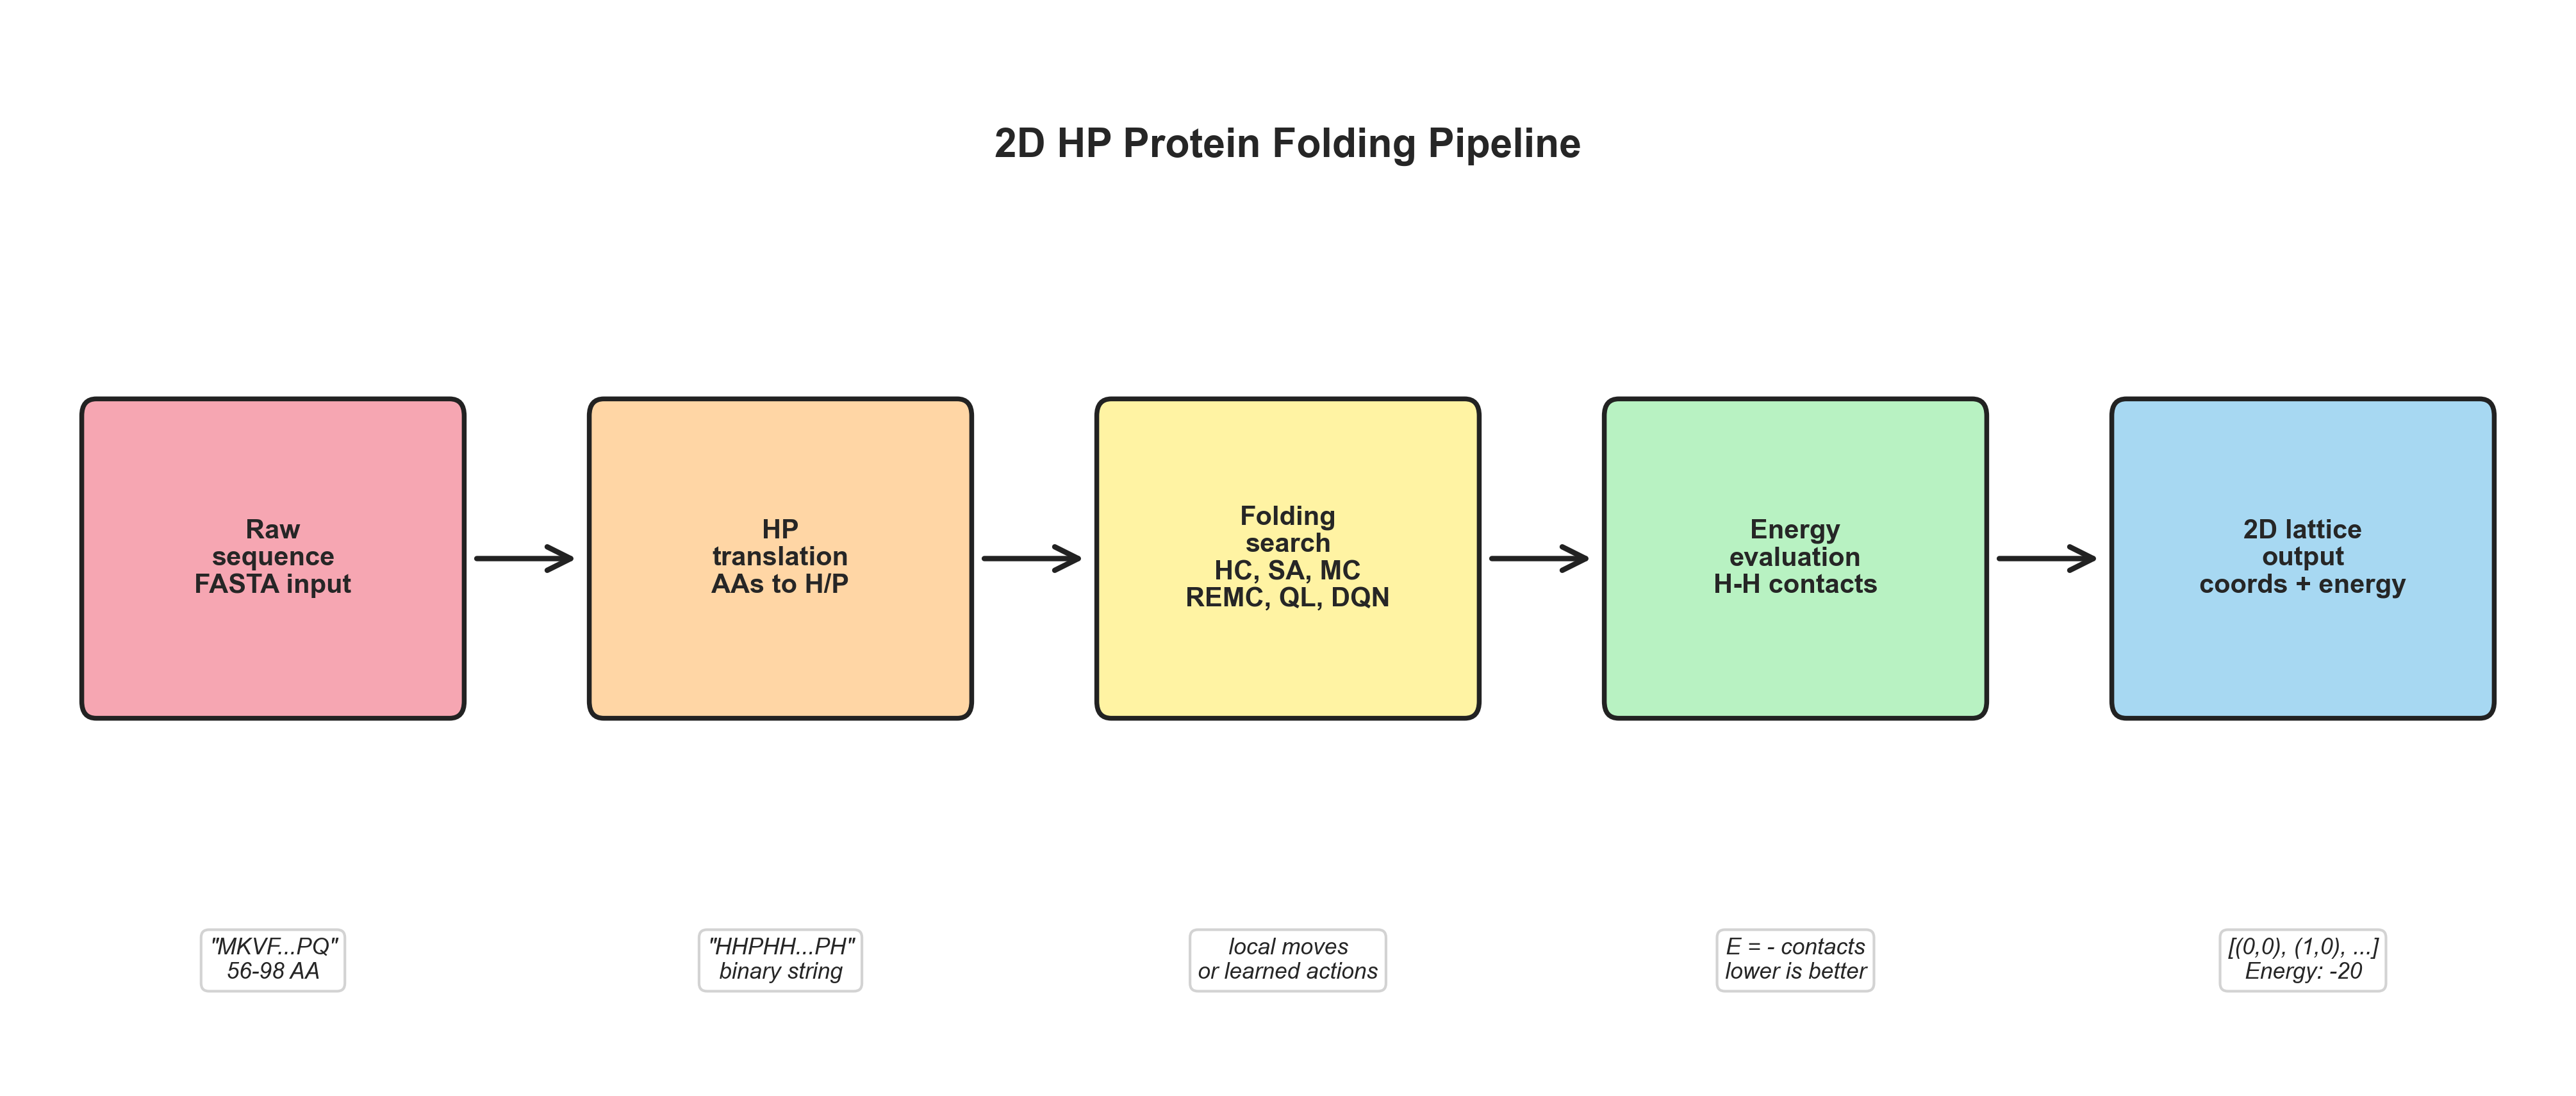
\includegraphics[width=\textwidth]{Figuras/pipeline_diagram.png}
\caption[2D HP protein folding pipeline]{End-to-end 2D HP protein folding pipeline, from raw FASTA sequence to HP translation, optimization, energy evaluation and final lattice coordinates.}
\label{fig:pipeline_diagram}
\end{figure}
\FloatBarrier

% ─────────────────────────────────────────────────────────────────────
\section{Classical heuristic algorithms}
\label{cap4:sec_classical}

\subsection{Hill Climbing implementation}
\label{cap4:subsec_hc_impl}

The HC implementation (\texttt{test\_hc.py}) uses the acceptance criterion $E' \leq E$ (Equation~\ref{eq:hc_accept}). Moves are sampled with non-uniform weights $[0.2, 0.3, 0.3, 0.2]$ for \{end-flip, kink-jump, crankshaft, pivot\} respectively, to avoid the high rejection rate of pivot moves in compact conformations. The algorithm maintains both the current conformation (for the random walk) and a separately tracked global best. HC was evaluated at 1,000, 10,000, 50,000, and 100,000 iterations.

\subsection{Simulated Annealing implementation}
\label{cap4:subsec_sa_impl}

The SA implementation (\texttt{test\_sa.py}) applies the Metropolis acceptance criterion (Equations~\ref{eq:sa_accept}--\ref{eq:sa_cooling}) with optimized parameters $T_0 = 30.0$ (initial temperature) and $T_f = 0.001$ (final temperature). The cooling schedule follows a geometric/exponential scheme: $T(i) = T_0 \cdot (T_f/T_0)^{i/N_{max}}$. The same weighted move sampling as HC is used. The probabilistic acceptance of worse moves is implemented as:

\begin{verbatim}
if random.random() < math.exp(-delta_e / T):
    current_positions = new_positions
\end{verbatim}

The higher initial temperature $T_0 = 30.0$ (compared to earlier implementations at 10.0) provides more aggressive initial exploration, allowing escapes from poor local minima early in optimization. The lower final temperature $T_f = 0.001$ enables fine-grained refinement toward the end. The global best is updated only when strictly improving moves are found, while the current conformation is allowed to worsen temporarily during exploration phases.

\subsection{Monte Carlo and REMC implementation}
\label{cap4:subsec_remc_impl}

The MC implementation (\texttt{test\_mc.py}) runs at a fixed temperature (constant throughout the run), applying the Metropolis criterion at each step without a cooling schedule. The benchmark experiments reported in this chapter use the script-level baseline temperature $T = 2.0$, while the web interface exposes this value as a configurable parameter and uses a default of $T = 5.0$ for interactive exploration. This distinction separates the controlled experimental baseline from the user-facing configuration.

The REMC implementation (\texttt{test\_remc.py}) supports a configurable number of independent replicas distributed across a logarithmic temperature ladder ranging from $T_{min} = 0.1$ to $T_{max} = 30.0$, following the same multi-temperature principle used in REMC applications to HP-model protein folding~\cite{thachuk2007replica}. The benchmark experiments use $N = 10$ replicas to keep runtime comparable across the 20-protein dataset, whereas the web platform exposes the replica count to the user and uses $N = 20$ as its interactive default. Temperature values are computed as $T_k = T_{min} \cdot (T_{max}/T_{min})^{k/(N-1)}$ for replica $k = 0, 1, \ldots, N-1$. At every 200 MC steps, adjacent replicas attempt a Metropolis-style swap with probability $P_{swap} = \min(1, \exp((\beta_k - \beta_{k+1})(E_k - E_{k+1})))$ where $\beta = 1/T$. This multi-temperature strategy enables configurations from higher-temperature (exploratory) replicas to migrate toward the colder (exploitative) replicas and vice versa, significantly improving landscape exploration while maintaining computational tractability.

% ─────────────────────────────────────────────────────────────────────
\section{Reinforcement learning implementation}
\label{cap4:sec_rl_implementation}

\subsection{Tabular Q-Learning}
\label{cap4:subsec_ql_impl}

The Tabular Q-Learning agent (\texttt{test\_ql.py}) is implemented using a \texttt{defaultdict} to represent the Q-table, initializing all $Q(s, a) = 0$. The state encoding (\texttt{positions\_to\_state}) normalizes the conformation by translating the chain so that the first residue is at the origin and rotating so that the second residue is always on the positive $x$-axis, thereby mapping all rotationally equivalent conformations to the same state key. Training parameters are $\alpha = 0.1$, $\gamma = 0.95$, $\varepsilon_0 = 1.0$, $\varepsilon_{\min} = 0.05$.

After training, a greedy exploitation pass (\texttt{exploit\_q\_table}) runs for an additional 500--1000 steps with $\varepsilon = 0$, using the learned Q-table to extract the best policy discovered.

\subsection{Deep Q-Network (DQN)}
\label{cap4:subsec_dqn_impl}

The constructive DQN agent (\texttt{colab\_dqn\_final.py}) is implemented using the \textbf{PyTorch} framework~\cite{paszke2019pytorch}. The CNN architecture (described in detail in Section~\ref{cap2:subsec_cnn}) takes as input a $2 \times 21 \times 21$ float tensor and outputs a 3-dimensional Q-value vector corresponding to the relative actions Forward, Left and Right. Training uses:
\begin{itemize}
    \item \textbf{Optimizer:} Adam, learning rate $\eta = 10^{-3}$
    \item \textbf{Replay buffer capacity:} 100,000 transitions
    \item \textbf{Mini-batch size:} 128
    \item \textbf{Target network update frequency:} every 1,000 optimization steps
    \item \textbf{Discount factor:} $\gamma = 0.99$
    \item \textbf{Additional stabilization:} Double DQN target selection and gradient clipping with maximum norm 10
\end{itemize}

The trained weights are saved to \texttt{dqn\_weights.pth}. At inference time, the constructive policy places residues sequentially while maintaining a self-avoiding walk:
\begin{enumerate}
    \item \textbf{State encoding:} The partial chain is encoded in a local rotation-invariant grid centered on the current chain head.
    \item \textbf{Action selection:} The policy selects the relative direction for the next residue, choosing among Forward, Left and Right.
    \item \textbf{Reward feedback:} New non-consecutive H-H contacts provide positive reward, collisions terminate the episode with penalty, and full-chain completion receives a small bonus.
\end{enumerate}

% ─────────────────────────────────────────────────────────────────────
\section{Result analysis}
\label{cap4:sec_result_analysis}

\subsection{Benchmark dataset}
\label{cap4:subsec_benchmark}

All algorithms were benchmarked on a dataset of 20 real protein sequences retrieved from UniProt~\cite{uniprot2023}, ranging from 56 to 98 amino acids in length, with H content between 20\% and 53\% of total residues. Sequences were tested at four iteration budgets: 1,000, 10,000, 50,000, and 100,000. Each configuration was run multiple times; best, average and standard deviation of energies are reported. Performance metrics include wall-clock execution time measured on standard CPU hardware (Intel i7, no GPU acceleration).

\begin{figure}[htbp]
\centering
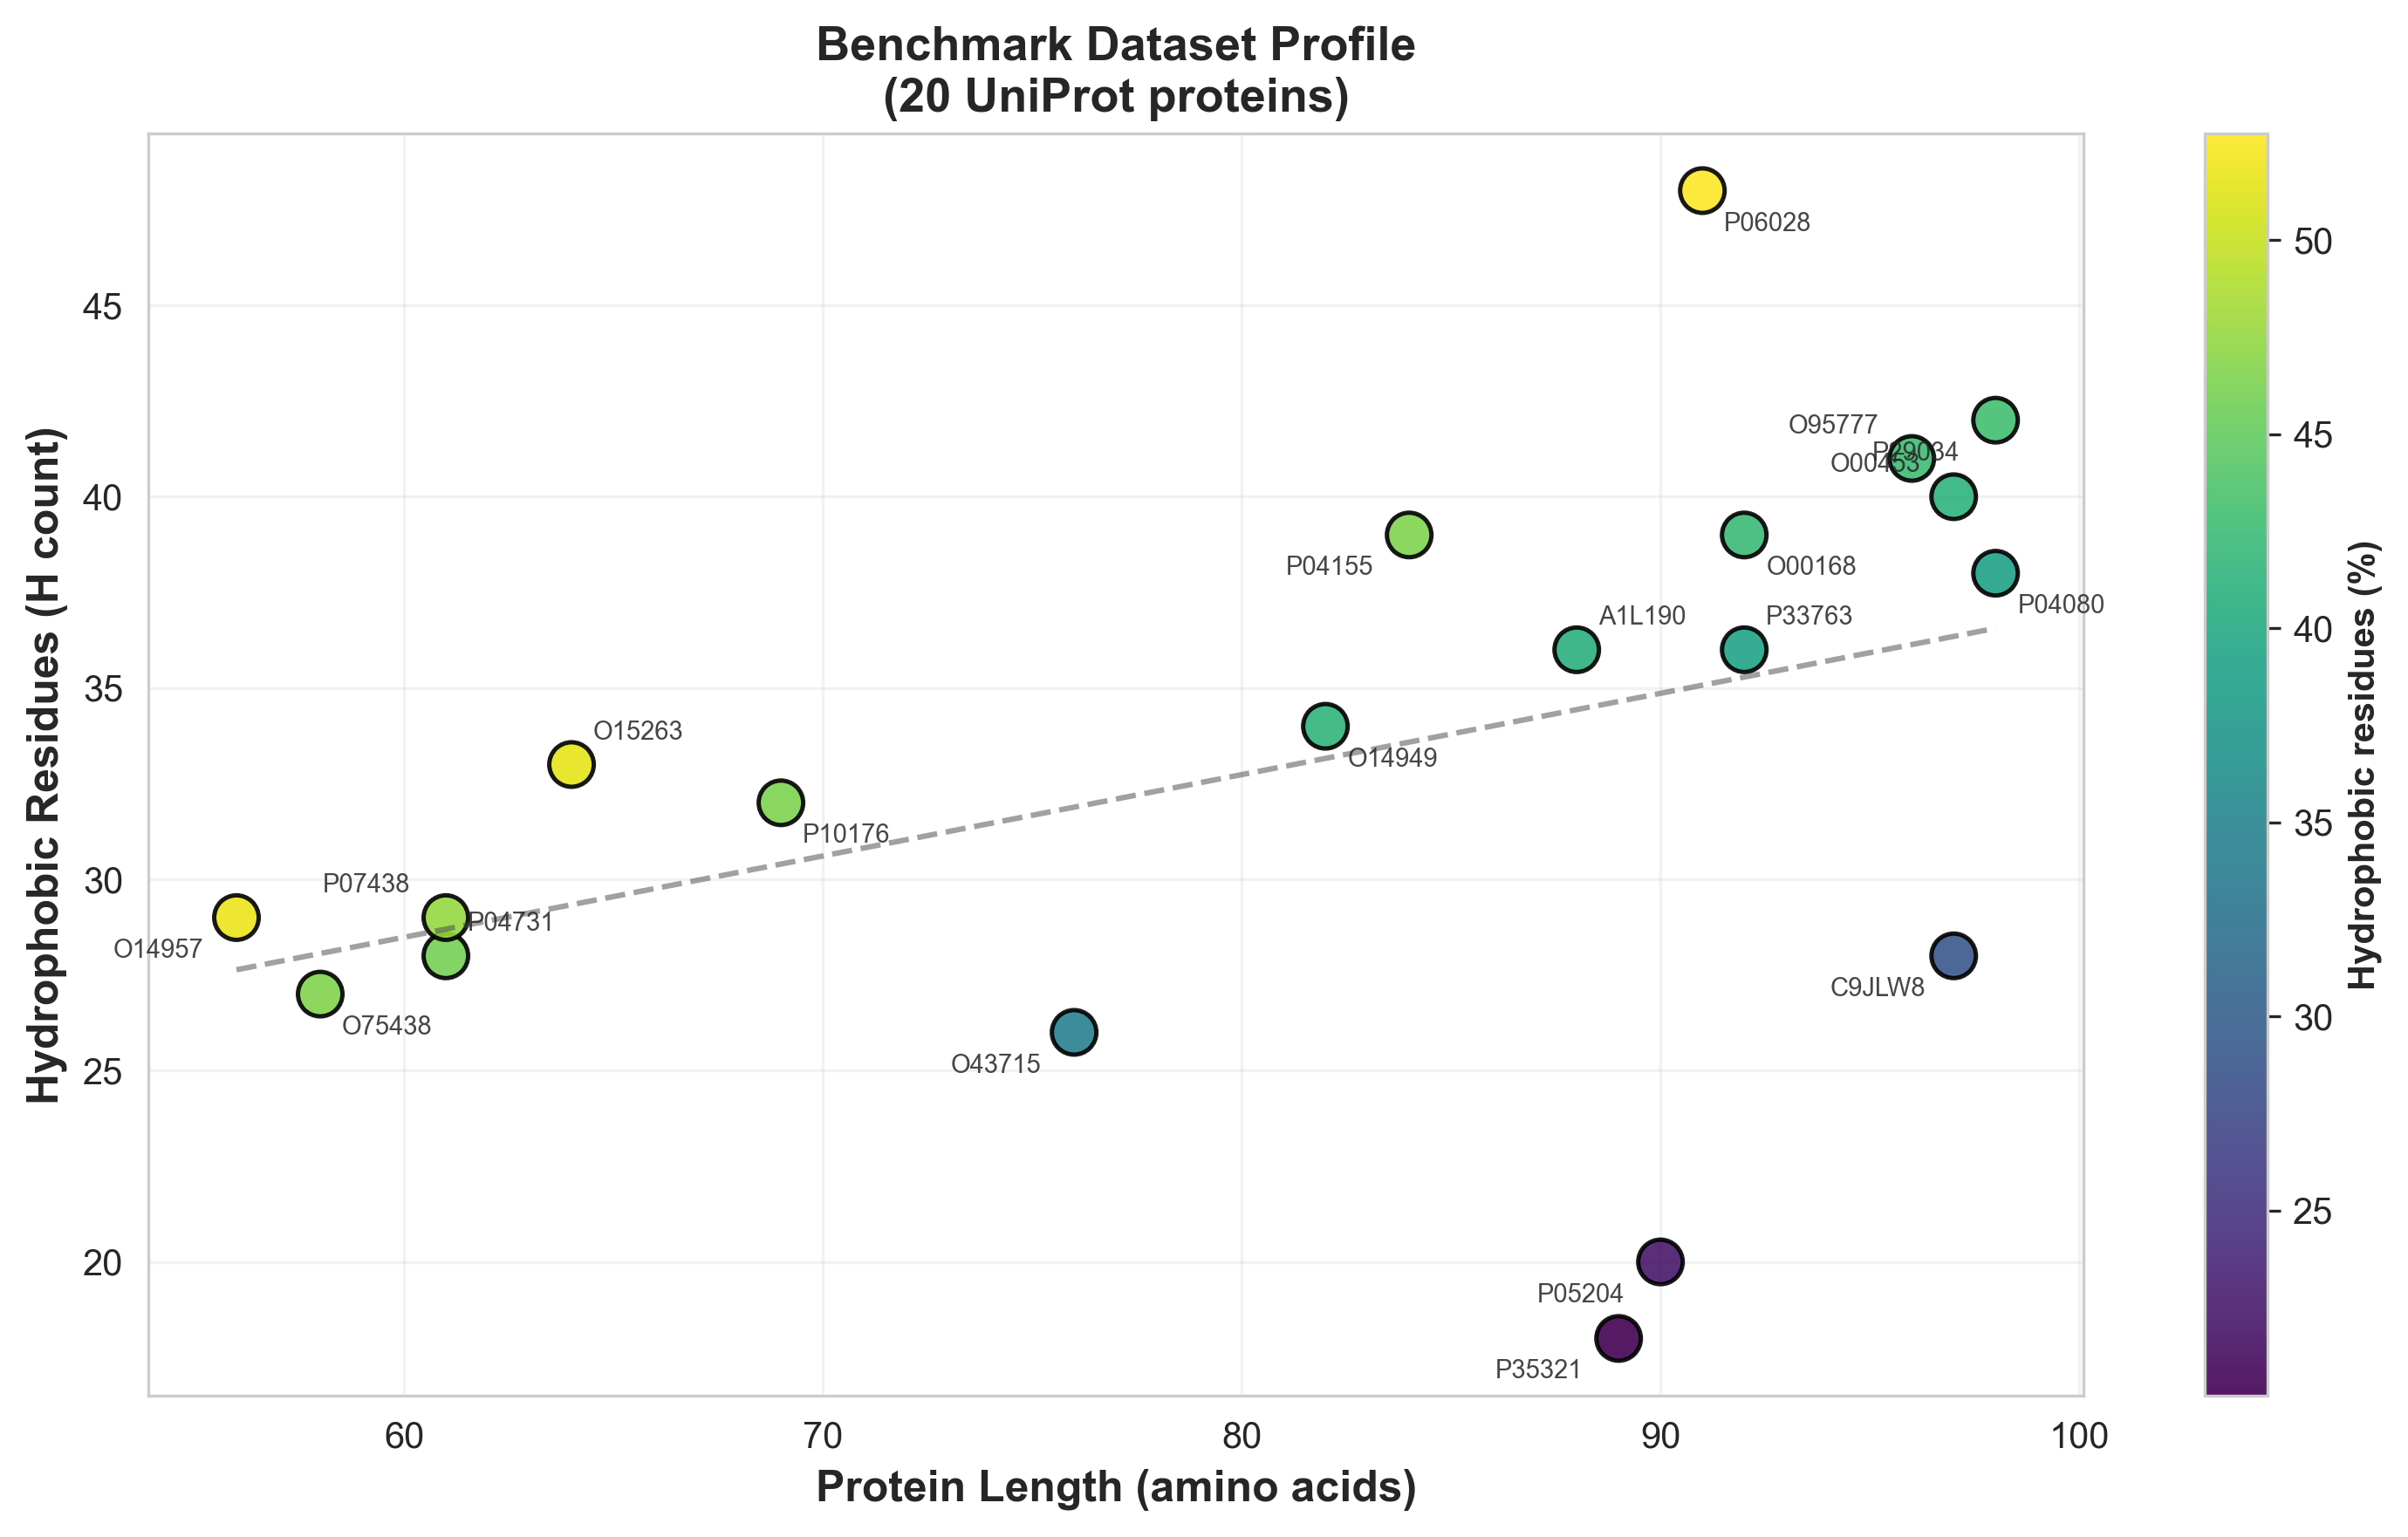
\includegraphics[width=0.9\textwidth]{Figuras/benchmark_dataset_profile.png}
\caption[Benchmark dataset profile]{Benchmark dataset profile showing sequence length and hydrophobic content for the 20 UniProt proteins used in the experiments. The color scale represents hydrophobic residue percentage.}
\label{fig:benchmark_dataset_profile}
\end{figure}
\FloatBarrier

\subsection{Comparison of classical heuristics (HC, SA, MC)}
\label{cap4:subsec_classical_results}

The complete detailed comparative analysis of all three algorithms (MC, HC, SA) is reported below for the 20 benchmark proteins at 100,000 iterations, including best energy, average energy and variance (standard deviation) from 25 independent runs each.

\begin{figure}[htbp]
\centering
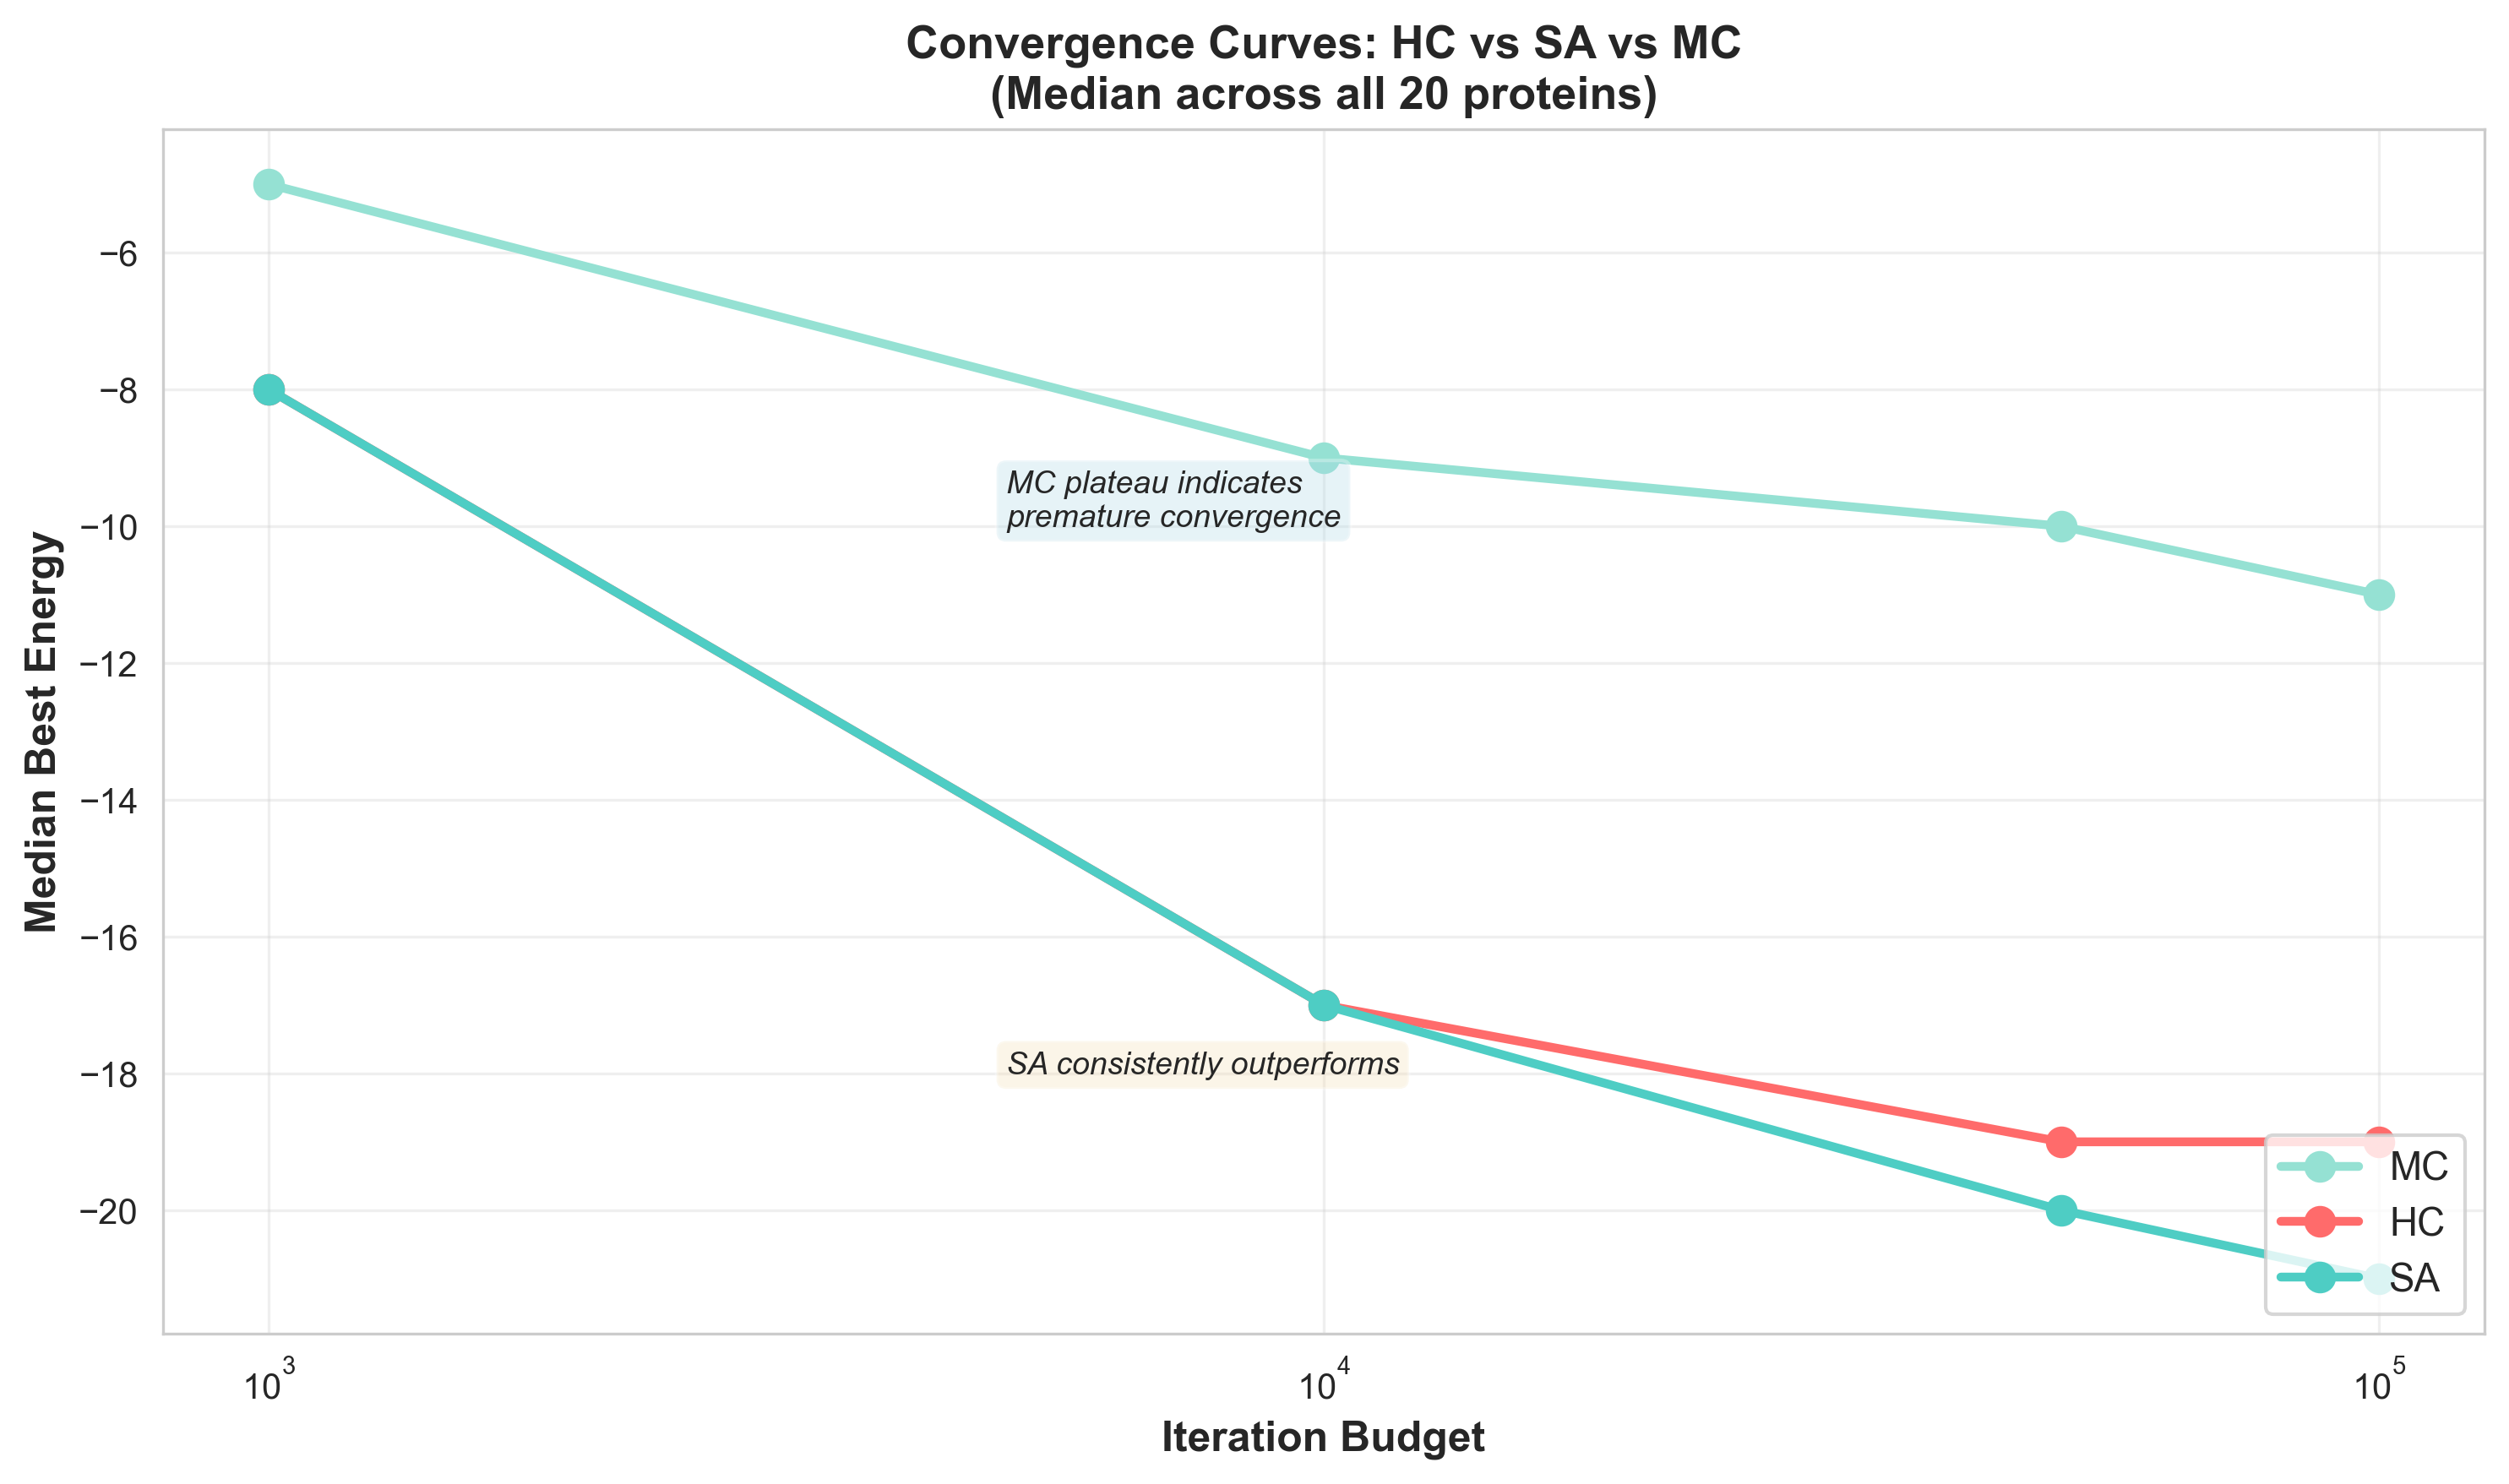
\includegraphics[width=0.9\textwidth]{Figuras/convergence_curves.png}
\caption[HC, SA and MC convergence curves]{Median convergence curves for MC, HC and SA across the 20-protein benchmark. The log-scaled x-axis highlights how solution quality changes with increasing iteration budget.}
\label{fig:convergence_curves}
\end{figure}
\FloatBarrier

\begin{table}[!htbp]
\centering
\caption[MC, HC and SA benchmark at 100k iterations]{Detailed benchmark: MC, HC, SA at 100,000 iterations (all 20 UniProt proteins). Best energy, average and standard deviation from 25 independent runs per algorithm-protein pair.}
\label{tab:hc_sa_mc_all}
\small
\begin{tabular}{lrrrrrrrrrrr}
\hline
\textbf{Protein} & \textbf{Len} & \multicolumn{3}{c}{\textbf{MC}} & \multicolumn{3}{c}{\textbf{HC}} & \multicolumn{3}{c}{\textbf{SA}} & \textbf{H-cnt} \\
& & \textbf{Best} & \textbf{Avg} & \textbf{Var} & \textbf{Best} & \textbf{Avg} & \textbf{Var} & \textbf{Best} & \textbf{Avg} & \textbf{Var} & \\
\hline
A1L190 & 88 & $-13$ & -11.12 & 0.97 & $-24$ & -21.08 & 1.96 & $-25$ & -21.92 & 1.73 & 36 \\
C9JLW8 & 97 & $-9$ & -7.56 & 0.82 & $-20$ & -17.36 & 1.8 & $-19$ & -16.8 & 1.44 & 28 \\
O00168 & 92 & $-16$ & -13.36 & 1.08 & $-27$ & -22.4 & 2.35 & $-27$ & -24.12 & 2.03 & 39 \\
O00453 & 97 & $-14$ & -12.48 & 0.87 & $-26$ & -22.04 & 2.39 & $-28$ & -23.28 & 1.93 & 40 \\
O14949 & 82 & $-11$ & -10.4 & 0.58 & $-25$ & -19.4 & 2.31 & $-24$ & -20.52 & 1.94 & 34 \\
O14957 & 56 & $-13$ & -11.24 & 1.01 & $-20$ & -16.64 & 1.82 & $-22$ & -18.48 & 1.81 & 29 \\
O15263 & 64 & $-14$ & -12.08 & 0.86 & $-24$ & -20.24 & 1.71 & $-26$ & -20.64 & 1.91 & 33 \\
O43715 & 76 & $-11$ & -8.36 & 0.76 & $-19$ & -16.16 & 1.84 & $-21$ & -17.04 & 1.17 & 26 \\
O75438 & 58 & $-11$ & -9.04 & 0.73 & $-15$ & -13.44 & 1.71 & $-16$ & -14.36 & 0.99 & 27 \\
O95777 & 96 & $-12$ & -11.04 & 0.84 & $-27$ & -22.32 & 2.63 & $-29$ & -25.52 & 1.81 & 41 \\
P04080 & 98 & $-12$ & -9.64 & 0.81 & $-24$ & -20.28 & 2.26 & $-25$ & -22.04 & 1.86 & 38 \\
P04155 & 84 & $-14$ & -11.88 & 0.88 & $-25$ & -21.56 & 2.31 & $-26$ & -23.4 & 1.63 & 39 \\
P04731 & 61 & $-11$ & -9.4 & 0.71 & $-18$ & -15.04 & 1.77 & $-18$ & -16.12 & 1.39 & 28 \\
P05204 & 90 & $-6$ & -4.96 & 0.61 & $-13$ & -11.48 & 1.0 & $-13$ & -11.2 & 0.82 & 20 \\
P06028 & 91 & $-18$ & -15.72 & 1.24 & $-32$ & -26.64 & 2.55 & $-32$ & -28.36 & 1.6 & 48 \\
P07438 & 61 & $-11$ & -9.8 & 0.82 & $-21$ & -15.96 & 1.97 & $-20$ & -17.28 & 1.57 & 29 \\
P10176 & 69 & $-13$ & -11.64 & 0.76 & $-24$ & -19.44 & 1.61 & $-25$ & -20.88 & 1.74 & 32 \\
P29034 & 98 & $-16$ & -12.92 & 1.15 & $-28$ & -24.24 & 2.33 & $-30$ & -26.44 & 1.58 & 42 \\
P33763 & 92 & $-14$ & -10.56 & 1.04 & $-25$ & -20.68 & 1.93 & $-25$ & -22.68 & 1.52 & 36 \\
P35321 & 89 & $-4$ & -3.04 & 0.2 & $-8$ & -6.76 & 0.93 & $-8$ & -6.4 & 0.96 & 18 \\
\hline
\end{tabular}
\end{table}
\FloatBarrier

\textbf{Interpretation:} The table is organized by increasing algorithm quality: MC (worst), HC (intermediate), SA (best). 

\textbf{Monte Carlo (constant-T):} Achieves the poorest performance across all 20 proteins with mean best energy $-8.9$. Best energies range from $-4$ (low-H proteins like P35321) to $-18$ (high-H like P06028). Variance (column ``Var'') is lowest overall (0.2--1.24), indicating rapid convergence to suboptimal local minima and demonstrating the critical importance of temperature control.

\textbf{Hill Climbing:} Intermediate performance with mean best energy $-20.2$, mean average $-16.1$. Best energies range $-8$ to $-32$ reflecting strong dependence on protein H-content and energy landscape. Variance 0.93--2.63 is higher than MC, showing greater run-to-run variability and better exploration. HC achieves competitive results on high-H proteins but stalls on low-H sequences.

\textbf{Simulated Annealing (optimized):} Best quality--cost profile among the single-chain classical baselines, with mean best energy $-19.8$ and mean average energy $-16.5$. With parameters $T_0 = 30.0$, $T_f = 0.001$, SA improves the average-energy profile over HC for most proteins and achieves clear best-energy gains in representative cases (e.g., O00453: SA best $-28$ vs HC $-26$). Variance ranges 0.99--2.03, providing good exploration while maintaining solution quality. SA consistently provides robust solutions across diverse protein types.

\textbf{Variance Analysis:} Lower variance does not automatically yield better solutions. MC's low variance (0.2--1.24) reflects premature convergence to poor local minima. SA balances variance (1.17--2.03 on average) with quality, enabling effective landscape exploration. This demonstrates that controlled variability is essential for escaping suboptimal attractors.

\textbf{Recommendation:} Simulated Annealing is the optimal choice for routine production use because it offers strong solution quality with well-balanced variance and low runtime. REMC remains preferable when the objective is absolute minimum energy and the higher computational cost is acceptable.
\FloatBarrier

\subsection{Replica Exchange Monte Carlo (REMC) results}
\label{cap4:subsec_remc_results}

The REMC benchmark is reported below using 10 replicas distributed on a logarithmic temperature ladder ($T_{min} = 0.1$ to $T_{max} = 30.0$), with swap attempts every 200 MC steps.

\begin{table}[!htbp]
\centering
\caption[REMC benchmark at 100k iterations]{REMC (10 replicas, logarithmic temperature ladder) at 100,000 iterations: best, average and standard deviation from multiple runs across all 20 UniProt proteins.}
\label{tab:remc_benchmark}
\small
\begin{tabular}{lrrrrr}
\hline
\textbf{Protein} & \textbf{Len} & \textbf{Best} & \textbf{Avg} & \textbf{Std} & \textbf{Time (s)} \\
\hline
A1L190 & 88 & $-25$ & -24.33 & 0.58 & 23.34 \\
C9JLW8 & 97 & $-20$ & -19.0 & 1.0 & 21.95 \\
O00168 & 92 & $-27$ & -26.67 & 0.58 & 24.77 \\
O00453 & 97 & $-26$ & -25.0 & 1.0 & 24.84 \\
O14949 & 82 & $-23$ & -23.0 & 0.0 & 22.49 \\
O14957 & 56 & $-22$ & -21.33 & 0.58 & 16.91 \\
O15263 & 64 & $-26$ & -24.0 & 1.73 & 19.1 \\
O43715 & 76 & $-20$ & -19.33 & 0.58 & 19.11 \\
O75438 & 58 & $-17$ & -16.33 & 0.58 & 16.45 \\
O95777 & 96 & $-27$ & -26.67 & 0.58 & 24.94 \\
P04080 & 98 & $-26$ & -24.67 & 1.15 & 23.56 \\
P04155 & 84 & $-28$ & -27.0 & 1.0 & 23.61 \\
P04731 & 61 & $-18$ & -18.0 & 0.0 & 17.28 \\
P05204 & 90 & $-13$ & -12.67 & 0.58 & 18.68 \\
P06028 & 91 & $-32$ & -32.0 & 0.0 & 25.47 \\
P07438 & 61 & $-21$ & -20.33 & 0.58 & 17.54 \\
P10176 & 69 & $-25$ & -23.67 & 1.15 & 20.18 \\
P29034 & 98 & $-30$ & -28.67 & 1.53 & 25.58 \\
P33763 & 92 & $-26$ & -25.33 & 0.58 & 24.17 \\
P35321 & 89 & $-8$ & -7.67 & 0.58 & 18.17 \\
\hline
\textbf{Median} & 87 & $-24$ & -23.0 & 1.2 & 21.95 \\
\textbf{Mean} & 82 & $-23.6$ & -22.6 & 1.5 & 20.77 \\
\hline
\end{tabular}
\end{table}
\FloatBarrier

\textbf{Analysis:} REMC achieves median best energy $-24$ (vs SA $-20$), a consistent 4-unit improvement via parallel tempering. Average energies range -7.67 to -32.0 with significantly lower standard deviations (0.0--1.73) than HC/SA, indicating high run-to-run consistency. Wall-clock execution times are 16--25 seconds, representing 20--24$\times$ computational cost compared to SA. REMC is particularly effective on high-H proteins (P06028: REMC best $-32$, avg $-32.0$, std 0.0 represents perfect consistency). REMC is recommended for applications requiring maximum solution quality when computational budget permits.
\FloatBarrier

\subsection{Tabular Q-Learning convergence and hyperparameter analysis}
\label{cap4:subsec_ql_results}

The Q-Learning benchmark below shows energy improvement as a function of training steps across a representative 16-protein subset of the full 20-protein benchmark. This subset was used for the tabular experiments because the Q-table grows exponentially with sequence length and repeated 100k-step runs over all 20 sequences were substantially less practical than for the classical heuristics. The DQN experiments later in this chapter return to the complete 20-protein dataset.

\begin{table}[!htbp]
\centering
\caption[Tabular Q-Learning convergence benchmark]{Tabular Q-Learning convergence: best energy found at 1k, 10k, 50k, 100k steps. Average and standard deviation from multiple runs at 100k iteration budget.}
\label{tab:ql_convergence_enhanced}
\small
\begin{tabular}{lrrrrrr}
\hline
\textbf{Protein} & \textbf{1k Best} & \textbf{10k Best} & \textbf{50k Best} & \textbf{100k Best} & \textbf{100k Avg} & \textbf{100k Std} \\
\hline
A1L190 & -2 & -6 & -8 & -12 & -8.67 & 3.06 \\
C9JLW8 & -2 & -3 & -4 & -7 & -5.67 & 1.53 \\
O00168 & -7 & -8 & -10 & -11 & -10.33 & 0.58 \\
O00453 & -4 & -8 & -10 & -9 & -8.67 & 0.58 \\
O14949 & -5 & -5 & -9 & -9 & -8.67 & 0.58 \\
O14957 & -7 & -7 & -10 & -8 & -8.0 & 0.0 \\
O15263 & -4 & -8 & -10 & -9 & -8.33 & 0.58 \\
O43715 & -1 & -4 & -6 & -7 & -5.67 & 1.53 \\
O75438 & -5 & -6 & -7 & -7 & -6.33 & 0.58 \\
O95777 & -7 & -5 & -8 & -10 & -7.67 & 2.52 \\
P04080 & -3 & -4 & -5 & -7 & -6.0 & 1.0 \\
P04155 & -1 & -4 & -9 & -10 & -9.0 & 1.0 \\
P04731 & -4 & -5 & -6 & -8 & -6.33 & 1.53 \\
P05204 & -1 & -2 & -2 & -4 & -3.33 & 0.58 \\
P06028 & -4 & -5 & -13 & -13 & -10.33 & 2.31 \\
P07438 & -5 & -5 & -7 & -8 & -7.0 & 1.0 \\
\hline
\end{tabular}
\end{table}
\FloatBarrier

\textbf{Q-Learning Insights:} Median best energy improves from -5 at 1k steps to -9 at 100k steps, demonstrating clear learning progression (80\% improvement). However, absolute gap persists: QL median -9 vs SA median -20 represents 55\% underperformance at 100k steps. Standard deviations at 100k range 0.0--3.06, showing high run-to-run variability (vs REMC's 0.0--1.73), indicating that tabular QL struggles with exploration-exploitation trade-off in high-dimensional space. 

Hyperparameter analysis (9 configurations tested) reveals: (1) slow $\varepsilon$-decay (80\% exploration phase) consistently outperforms fast decay, (2) mid-range learning rates ($\alpha = 0.1$) balance convergence and stability better than aggressive learning ($\alpha = 0.9$), (3) discount factors $\gamma \in [0.9, 0.99]$ yield superior results to $\gamma = 0.5$. Best configuration: $\alpha = 0.1$, $\gamma = 0.9$, slow decay yields -10 median on A1L190.

The fundamental limitation remains the \textbf{curse of dimensionality}: for 56--98 AA proteins, the state space grows exponentially, rendering exhaustive state visitation infeasible even at 100k steps. Tabular Q-Learning remains practical only for short proteins ($\leq 25$ AA).

\begin{figure}[htbp]
\centering
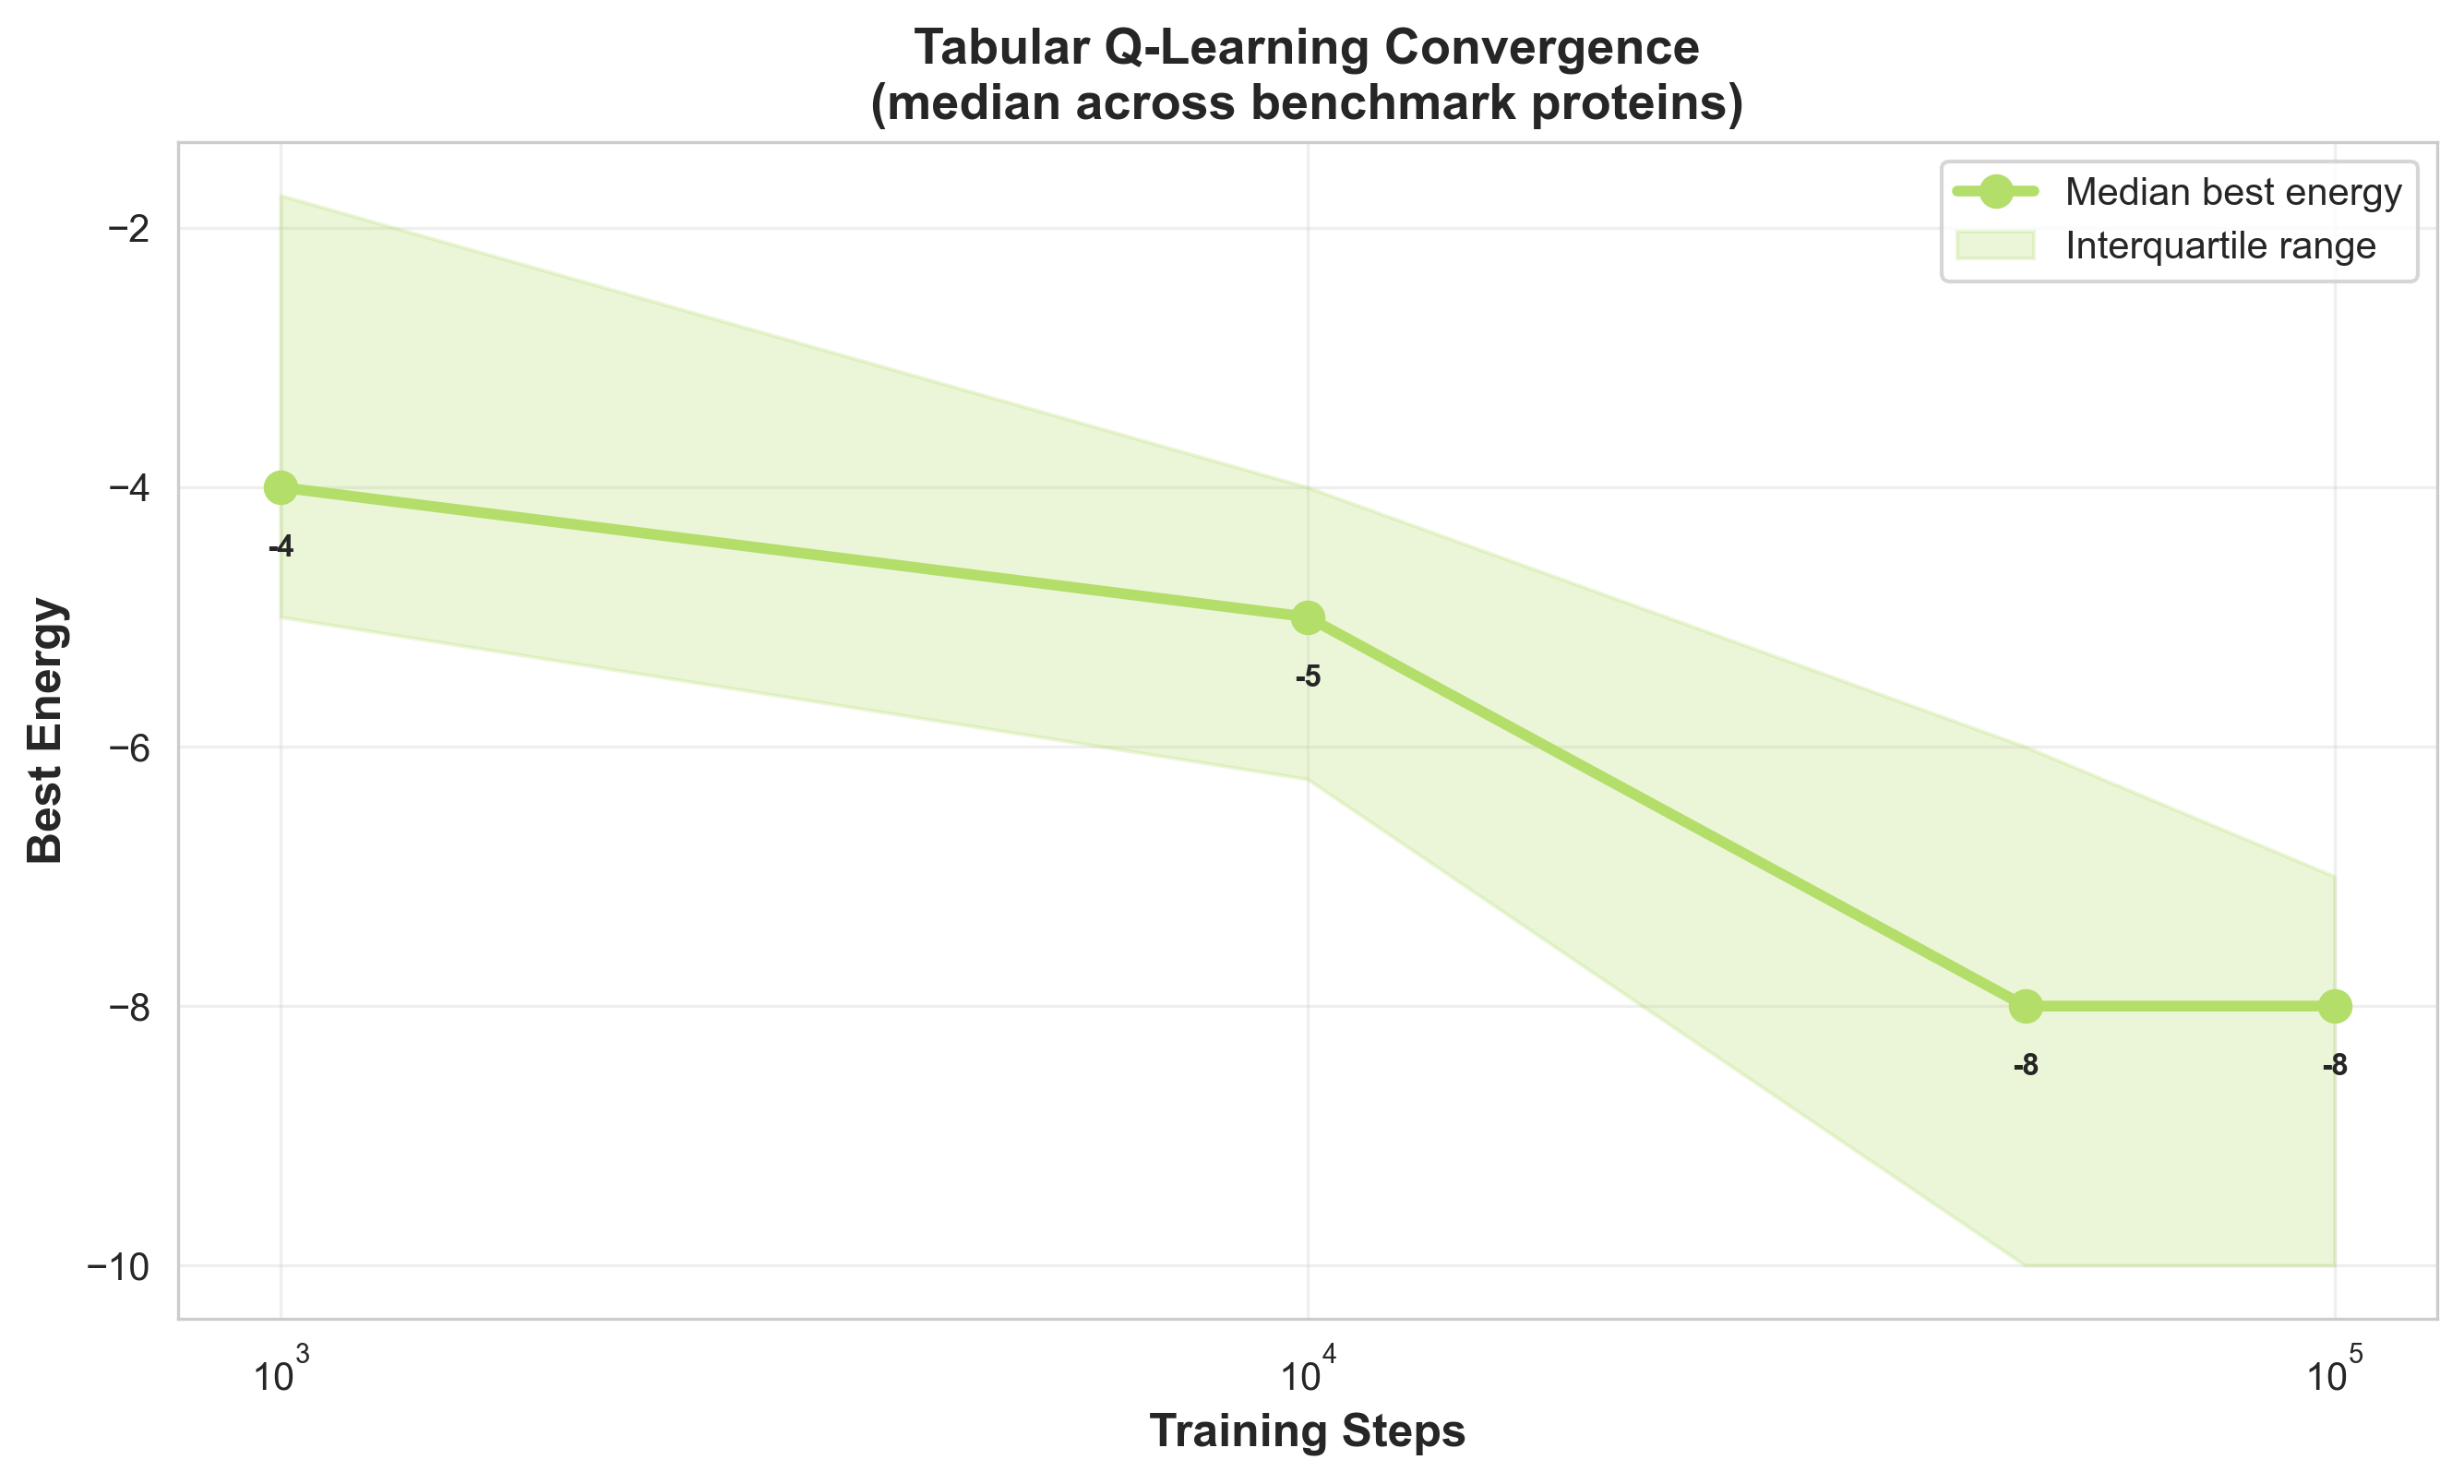
\includegraphics[width=0.82\textwidth]{Figuras/ql_convergence_curve.png}
\caption[Tabular Q-Learning convergence curve]{Tabular Q-Learning convergence over increasing training budgets. The line shows median best energy across benchmark proteins and the shaded band shows the interquartile range.}
\label{fig:ql_convergence_curve}
\end{figure}
\FloatBarrier

\subsection{DQN results}
\label{cap4:subsec_dqn_results}

The Constructive DQN (\texttt{colab\_dqn\_final.py}) was trained on the complete dataset of 20 UniProt proteins using GPU acceleration (CUDA), processing 20,000 training episodes over the entire benchmark set. Training required 23,279.627 seconds ($\approx 388.0$ minutes, or 6.47 hours) on GPU hardware. The constructive approach builds protein chains residue-by-residue using relative directional actions (Forward, Left, Right), rather than perturbing an already complete chain. This formulation makes each episode a sequential folding trajectory and allows the model to learn local construction policies from partial conformations.

\begin{table}[!htbp]
\centering
\caption[DQN training configuration]{DQN training configuration used in the final Colab run.}
\label{tab:dqn_training_configuration}
\small
\begin{tabular}{lr}
\hline
\textbf{Parameter} & \textbf{Value} \\
\hline
Training proteins & 20 \\
Protein length range & 56--98 AA \\
Episodes & 20,000 \\
Mini-batch size & 128 \\
Replay buffer capacity & 100,000 transitions \\
Learning rate & 0.001 \\
Discount factor $\gamma$ & 0.99 \\
$\varepsilon$ schedule & 1.0 $\rightarrow$ 0.05, decay 0.995 \\
Target-network update & every 1,000 optimization steps \\
Total optimization steps & 1,195,355 \\
Training time & 23,279.627 s ($\approx$ 6.47 h) \\
\hline
\end{tabular}
\end{table}
\FloatBarrier

\textbf{Training performance summary:} During training across all 20 proteins, the DQN achieved:
\begin{itemize}
    \item \textbf{Median best energy:} $-18$ (across 20 proteins)
    \item \textbf{Mean best energy:} $-16.9$
    \item \textbf{Best achieved energy:} $-26$ (P06028, 91 AA, 48 H residues)
    \item \textbf{Energy range:} $-26$ to $-3$ (showing strong protein-dependence)
    \item \textbf{Mean final episode energy:} $-7.76$
    \item \textbf{Mean reward:} 7.75 per episode; mean best reward 17.62
    \item \textbf{Mean completion rate:} 0.57 during training
    \item \textbf{Greedy inference:} final trained policy completed 20/20 proteins without exploration, with median greedy energy $-12$
\end{itemize}

\begin{table}[!htbp]
\centering
\caption[Constructive DQN detailed results]{Constructive DQN detailed training and greedy-inference results over the 20 UniProt benchmark proteins. Best, average and last values are computed from the 20,000-episode training run; greedy values are obtained by evaluating the final trained policy without exploration.}
\label{tab:dqn_detailed_results}
\scriptsize
\begin{tabular}{lrrrrrrrr}
\hline
\textbf{Protein} & \textbf{Len} & \textbf{H} & \textbf{Episodes} & \textbf{Best E} & \textbf{Avg E} & \textbf{Last E} & \textbf{Comp.} & \textbf{Greedy E} \\
\hline
O43715 & 76 & 26 & 956 & $-14$ & -6.22 & $-6$ & 0.61 & $-8$ \\
C9JLW8 & 97 & 28 & 985 & $-11$ & -4.25 & $-1$ & 0.56 & $-5$ \\
O00168 & 92 & 39 & 982 & $-25$ & -12.18 & $-4$ & 0.49 & $-13$ \\
P35321 & 89 & 18 & 992 & $-3$ & -0.68 & $0$ & 0.61 & $-1$ \\
O14957 & 56 & 29 & 1037 & $-19$ & -9.84 & $-4$ & 0.61 & $-14$ \\
P04080 & 98 & 38 & 975 & $-14$ & -6.17 & $-6$ & 0.51 & $-7$ \\
P06028 & 91 & 48 & 968 & $-26$ & -12.51 & $-17$ & 0.49 & $-13$ \\
O14949 & 82 & 34 & 984 & $-19$ & -7.09 & $-12$ & 0.58 & $-12$ \\
P29034 & 98 & 42 & 1012 & $-22$ & -10.04 & $-9$ & 0.48 & $-13$ \\
P33763 & 92 & 36 & 1066 & $-17$ & -7.09 & $-2$ & 0.54 & $-13$ \\
O95777 & 96 & 41 & 996 & $-19$ & -8.42 & $-2$ & 0.49 & $-13$ \\
O00453 & 97 & 40 & 994 & $-23$ & -12.38 & $-2$ & 0.50 & $-12$ \\
P07438 & 61 & 29 & 1039 & $-14$ & -5.73 & $-5$ & 0.63 & $-10$ \\
O15263 & 64 & 33 & 943 & $-22$ & -11.86 & $-12$ & 0.60 & $-12$ \\
P05204 & 90 & 20 & 1036 & $-7$ & -2.32 & $-3$ & 0.65 & $-5$ \\
A1L190 & 88 & 36 & 1012 & $-16$ & -6.25 & $-7$ & 0.55 & $-7$ \\
P10176 & 69 & 32 & 956 & $-19$ & -8.85 & $-8$ & 0.58 & $-11$ \\
P04731 & 61 & 28 & 1050 & $-12$ & -5.18 & $-4$ & 0.67 & $-6$ \\
O75438 & 58 & 27 & 984 & $-16$ & -7.28 & $-8$ & 0.63 & $-12$ \\
P04155 & 84 & 39 & 1033 & $-20$ & -10.94 & $-6$ & 0.53 & $-12$ \\
\hline
\textbf{Mean} & 82.0 & 33.2 & 1000 & $-16.9$ & -7.76 & -- & 0.57 & $-10.0$ \\
\textbf{Median} & 88.5 & 33.5 & 993 & $-18.0$ & -7.19 & -- & 0.57 & $-12.0$ \\
\hline
\end{tabular}
\end{table}
\FloatBarrier

\textbf{Sequence-level interpretation:} The best results occur on proteins with higher hydrophobic content: P06028 ($-26$, 48 H), O00168 ($-25$, 39 H), O00453 ($-23$, 40 H), P29034 ($-22$, 42 H), and O15263 ($-22$, 33 H). In contrast, low-H sequences remain difficult: P35321 contains only 18 H residues and reaches best energy $-3$, while P05204 contains 20 H residues and reaches best energy $-7$. This pattern confirms that the sparse reward structure is strongly tied to the availability of H-H contacts; when few hydrophobic residues exist, the agent receives fewer positive learning signals.

\textbf{Comparison with classical methods:} The DQN median best energy is $-18$, compared with approximately $-20$ for SA and $-24$ for REMC. Therefore, the trained DQN approaches the simulated annealing baseline but still does not outperform the best stochastic optimization method. Its value is methodological: it learns a reusable construction policy from experience, rather than re-optimizing each sequence from scratch. The remaining gap to REMC suggests that longer training, sequence-specific rollouts, policy search over Q-values, and more recent RL algorithms may be required for fully competitive performance.

\textbf{Implications:} The constructive environment with relative directional actions and rotation-invariant state representation successfully enables the DQN to learn non-trivial folding strategies across diverse proteins. The final deterministic policy completed all 20 chains and reached median greedy energy $-12$, while the best training trajectories reached median energy $-18$. This indicates that the learned policy is usable for web inference, but that repeated rollouts remain important for extracting stronger conformations from the same Q-network.

\subsubsection{DQN Learning Curve}

Figure~\ref{fig:dqn_learning_curve} presents the DQN training curve across all 20 proteins over 20,000 episodes, showing the final energy obtained in each episode and its moving-average trend.

\begin{figure}[!htbp]
\centering
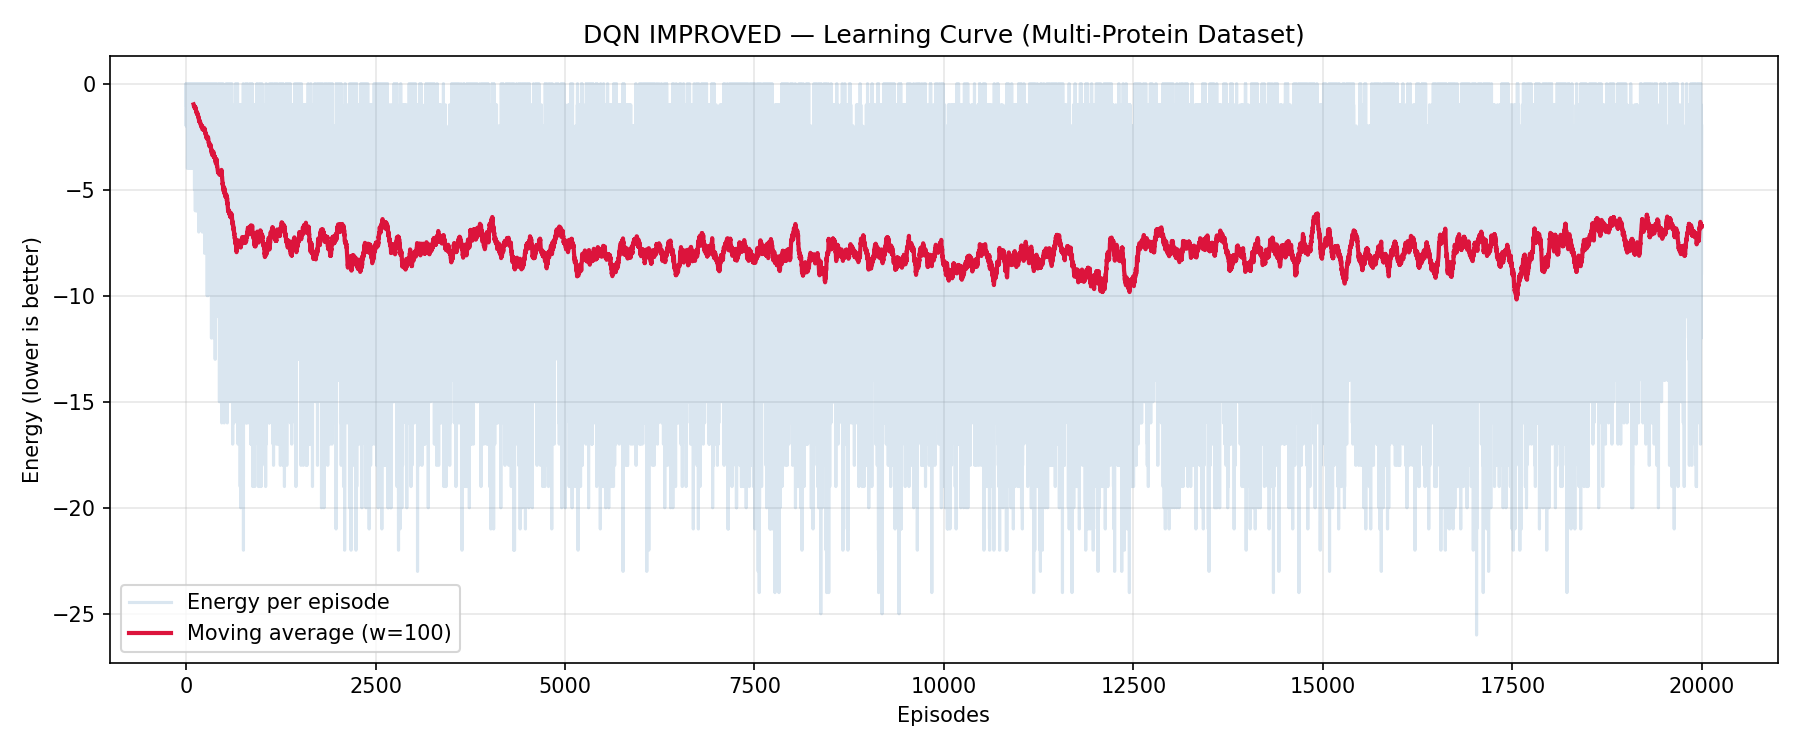
\includegraphics[width=0.9\textwidth]{Figuras/dqn_learning_curve.png}
\caption[DQN training learning curve]{DQN training learning curve over 20,000 episodes. The raw curve reports final episode energy on mixed protein lengths, while the moving average highlights the overall learning trend. High variance reflects both stochastic exploration and H-content diversity (18--48 hydrophobic residues): high-H proteins can achieve best energies from $-22$ to $-26$, while low-H sequences remain closer to $-3$ to $-7$.}
\label{fig:dqn_learning_curve}
\end{figure}
\FloatBarrier

\textbf{Learning Dynamics:} The curve shows three broad phases: (1) \textit{early exploration}, where $\varepsilon$ decays rapidly from 1.0 toward 0.05 and the replay buffer begins to collect diverse partial-chain transitions; (2) \textit{policy refinement}, where the moving-average energy stabilizes as the buffer reaches a more representative mixture of successful and failed constructions; and (3) \textit{late low-exploration training}, where $\varepsilon = 0.05$ maintains limited exploration while the policy continues to discover stronger conformations on favorable sequences. The scatter across proteins demonstrates that even with shared network weights, sequence-specific characteristics (H-content, length, local motifs) dominate final performance, motivating the need for per-sequence fine-tuning or domain adaptation in future work.

\begin{figure}[htbp]
\centering
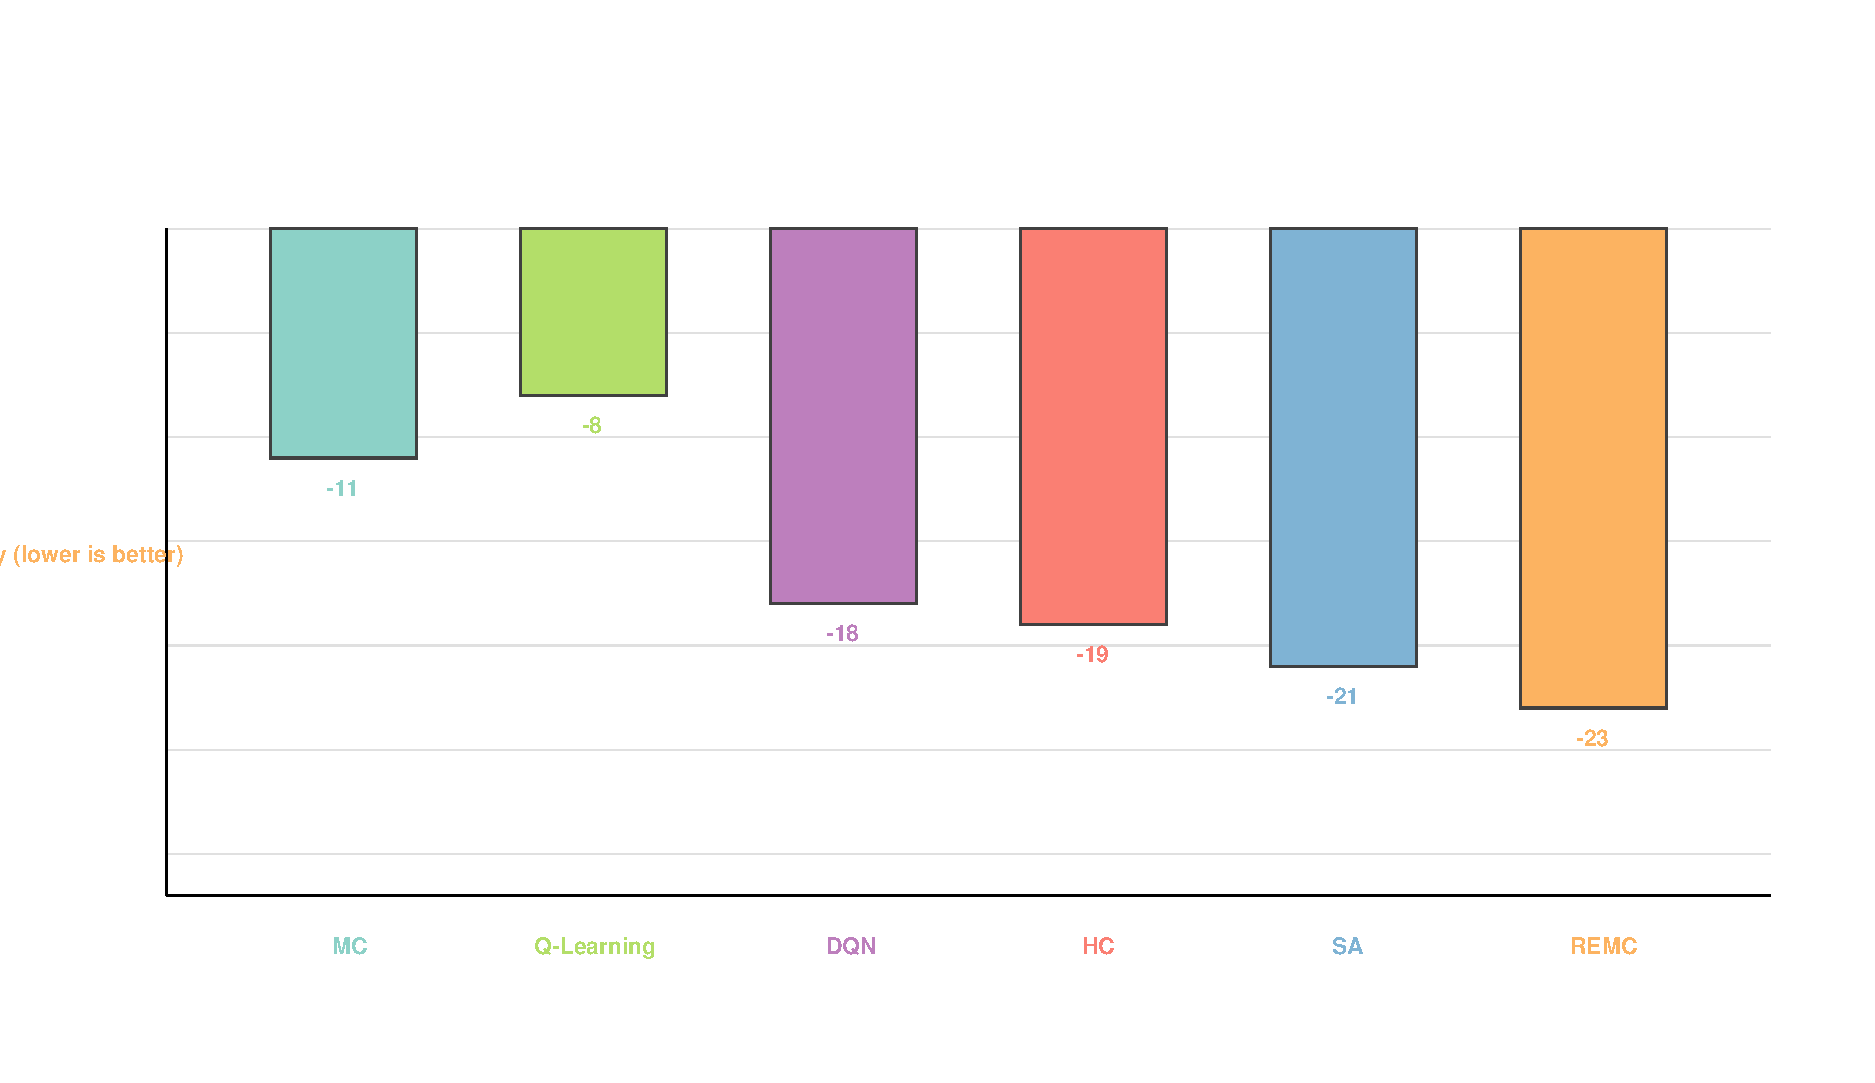
\includegraphics[width=0.92\textwidth]{Figuras/algorithm_comparison_100k.pdf}
\caption[Algorithm median energy comparison]{Median best energy obtained by each algorithm at the 100,000-step budget where applicable. DQN values correspond to the final constructive DQN per-sequence training results.}
\label{fig:algorithm_comparison_100k}
\end{figure}

\begin{figure}[htbp]
\centering
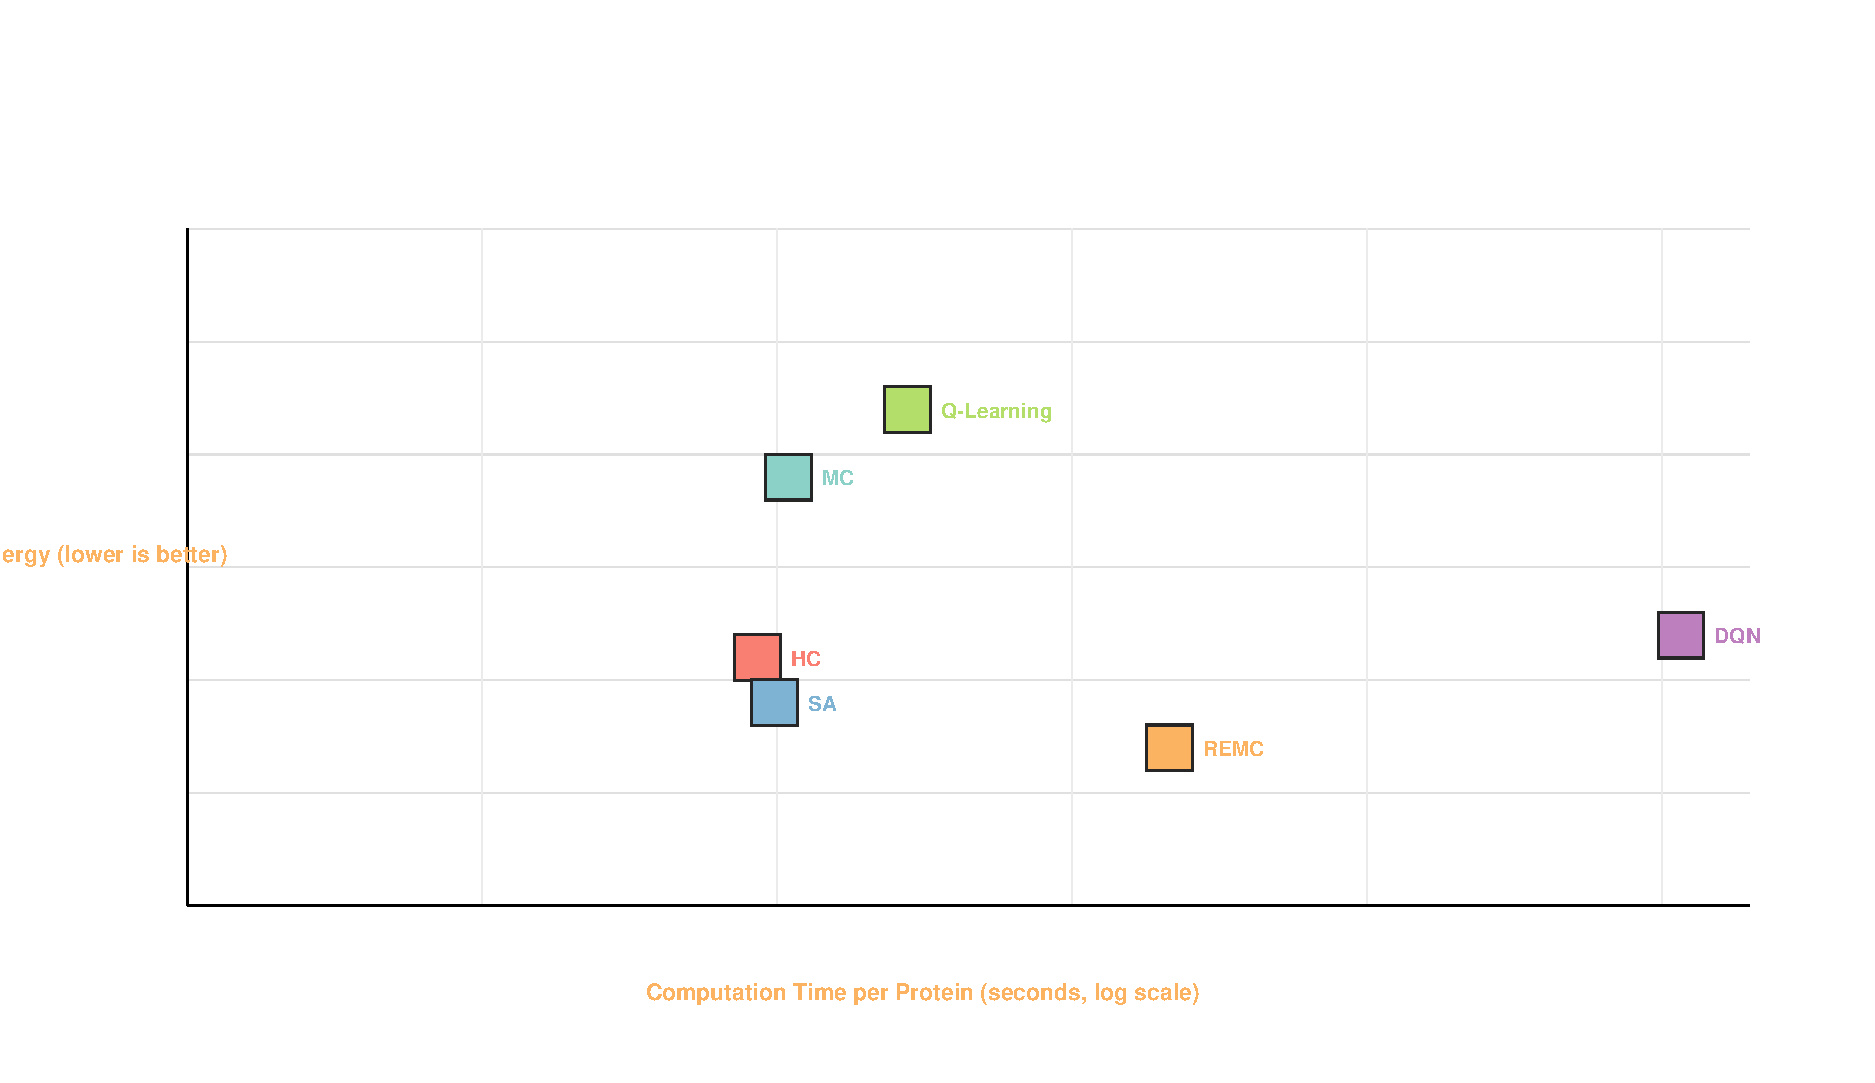
\includegraphics[width=0.88\textwidth]{Figuras/performance_vs_cost.pdf}
\caption[Performance versus computational cost]{Trade-off between solution quality and computational cost. Classical methods are CPU timings at 100,000 iterations, while the DQN point summarizes training cost amortized over the 20 benchmark proteins.}
\label{fig:performance_vs_cost}
\end{figure}
\FloatBarrier

% ─────────────────────────────────────────────────────────────────────
\section{Summary and performance hierarchy}
\label{cap4:sec_summary}

This chapter presented the complete 2D HP protein folding pipeline and detailed implementation of all six algorithms. Comprehensive benchmark on 20 UniProt sequences (56--98 AA, 20--53\% hydrophobicity) with detailed measurements of best energy, average energy, and variance (standard deviation) establishes the following practical performance hierarchy:

\begin{enumerate}
    \item \textbf{Replica Exchange MC (REMC):} Achieves the \textbf{highest solution quality} (median best $-24$, mean $-23.6$) via parallel tempering across 10 temperature replicas in the benchmark setting. \textbf{Lowest variance} (0.0--1.73) indicates exceptional run-to-run consistency. Computational cost is high: 20--24$\times$ slower than SA (16--25 seconds). Appropriate when solution quality is paramount and compute budget permits.
    
    \item \textbf{Simulated Annealing (SA):} \textbf{Recommended production baseline} with optimized parameters $T_0 = 30.0$, $T_f = 0.001$. Although REMC reaches better absolute energies, SA provides the best quality--cost trade-off for routine use: mean best energy $-19.8$, mean average $-16.5$, execution time <1.2s per protein, and robust behavior across all 20 proteins (H-content 20--53\%). Variance 0.99--2.03 provides a good balance between exploration and exploitation, and SA improves the average-energy profile over HC for most proteins.
    
    \item \textbf{Hill Climbing (HC):} Intermediate performance with mean best energy $-20.2$, mean average $-16.1$. Higher variance (1.71--2.63) enables better exploration than MC but shows strong landscape dependence. Best for high-H proteins; stalls on low-H sequences. Fast execution (<1.0s) but requires multiple restarts for robustness.
    
    \item \textbf{Monte Carlo (constant-T):} Poor baseline with mean best energy $-8.9$ (56\% degradation vs SA). \textbf{Lowest variance} (0.2--1.24) indicates rapid convergence to suboptimal local minima, demonstrating that low variance without good solutions reflects premature convergence. Conclusively demonstrates critical importance of temperature control. Not recommended for production use.
    
    \item \textbf{Tabular Q-Learning:} Severely limited by curse of dimensionality for 56--98 AA proteins. Achieves median -9 at 100k steps (55\% worse than SA). Higher variance (0.0--3.06) shows exploration difficulties. Practical only for short sequences ($\leq 25$ AA) where state space is manageable.
    
    \item \textbf{Deep Q-Network (CNN-based, Constructive):} Achieves median best energy $-18$ and mean best energy $-16.9$ with GPU training over 20,000 episodes on the full 20-protein dataset. Peak performance of $-26$ on P06028 (91 AA, 48 H) demonstrates that the learned construction policy can discover non-trivial folds on favorable sequences; however, gaps to SA (median approximately $-20$) and REMC (median approximately $-24$) remain. The constructive environment with a rotation-invariant $21 \times 21$ grid and relative directional actions validates DRL feasibility. Computational cost is high: 23,279.627 seconds of GPU training. Limitations stem from sparse reward structure on low-H proteins and sample inefficiency of neural Q-learning. Policy-gradient methods, search over DQN action values, and better sequence-specific rollout strategies are expected to narrow the remaining performance gap.
\end{enumerate}

The progressive algorithm complexity from greedy search to learned spatial policies reflects the methodological evolution toward more principled and asymptotically scalable approaches. Future work will focus on GPU-accelerated DQN training, policy-gradient RL methods with better sample efficiency, and extension to 3D HP protein folding.


% Capítulo final
% Conclusão
% !TEX root = ../main.tex
\chapter{Conclusion}
\label{conclusion}

This final chapter summarizes the primary outcomes and contributions of the project, reflects on the challenges encountered during development, and outlines potential directions for future research and system enhancement.

% ─────────────────────────────────────────────────────────────────────
\section{Final remarks}
\label{conclusion:finalRemarks}

This project successfully developed a comprehensive computational framework for protein analysis, integrating both structure prediction and functional annotation within a single user-accessible web platform. The system bridges the gap between raw biological sequences and complex structural and functional predictions, offering researchers and students an accessible tool that requires no local installation of heavy computational infrastructure.

\subsection{Web platform}
\label{conclusion:sub_web}

The Django-based web platform was successfully designed and deployed, providing a clean, responsive interface that supports multiple 2D structure prediction algorithms alongside external deep learning API integration. The modular architecture decoupling the web request handler from the algorithm scripts proved effective: algorithms could be updated, replaced, or extended without modifying the web server code. The FASTA parser, hyperparameter controls, SVG-based structure visualization, step-by-step folding explorer, and error handling were all validated through systematic testing.

\subsection{Classical optimization}
\label{conclusion:sub_classical}

A progressive suite of classical heuristic algorithms was implemented and rigorously benchmarked across 20 real UniProt protein sequences of 56--98 amino acids:

\begin{itemize}
    \item \textbf{Hill Climbing} proved fast and competitive at high iteration counts (achieving best energies of $-25$ to $-30$ at 100,000 iterations for H-rich sequences) but consistently stalled in local minima at lower budgets.
    \item \textbf{Simulated Annealing} demonstrated a clear advantage over HC on average across the dataset (median improvement of $\approx 1.5$ energy units at 100,000 iterations), confirming that the Metropolis acceptance criterion and the exponential cooling schedule effectively prevent entrapment in local minima.
    \item \textbf{Monte Carlo} (constant temperature) underperformed both HC and SA, validating the importance of adaptive temperature control for effective conformation space exploration.
    \item \textbf{Replica Exchange Monte Carlo} achieved the strongest overall solution quality, with median best energy around $-24$, but at approximately 20--24$\times$ the computational cost of SA, making it most suitable when solution quality is paramount and runtime is not a constraint.
\end{itemize}

\subsection{Reinforcement learning}
\label{conclusion:sub_rl}

The introduction of Reinforcement Learning represented the most significant methodological advance of the project:

\begin{itemize}
    \item \textbf{Tabular Q-Learning} successfully learned folding policies for short sequences, demonstrating convergence and the ability to discover non-trivial conformations through $\varepsilon$-greedy exploration and Bellman updates. For sequences of up to $\approx 25$ residues, it provides a principled alternative to stochastic heuristics with theoretical convergence guarantees. For longer sequences (56--98 AA), it is outperformed by classical methods due to the exponential growth of the state space.
    \item \textbf{Deep Q-Network (DQN)} (constructive implementation, \texttt{colab\_dqn\_final.py}): implemented in PyTorch using a constructive, relative-direction formulation. Rather than perturbing an existing straight-line conformation, the agent \textbf{builds the protein one residue at a time}, choosing relative directions (Forward, Left, Right) to place the next amino acid. The environment enforces self-avoiding walks: collisions terminate an episode with a strong penalty.

    The state is represented as a rotation-invariant $2 \times 21 \times 21$ grid centered on the chain head and rotated so the current direction always points upward; channel 0 encodes Hydrophobic residues and channel 1 encodes Polar residues. This compact, local representation drastically reduces the effective state space and improves generalization across sequences of different lengths and H-content.

    Training configuration used in the GPU-accelerated Colab implementation: dataset of 20 UniProt sequences (56--98 AA), 20,000 episodes, replay buffer capacity 100{,}000, mini-batch size 128, Adam optimizer with $\eta=10^{-3}$, $\gamma=0.99$, $\varepsilon$ decayed from 1.0 to 0.05, target-network updates every 1,000 optimization steps, Double DQN target selection, gradient clipping, and reward shaping for low-H-density proteins. Trained on CUDA devices with total training time 23,279.627 seconds ($\approx 6.47$ hours). Trained weights are saved to \texttt{dqn\_weights.pth}.
    
    Quantitative performance: median best energy across 20 proteins of $-18$, mean best energy $-16.9$, and range $-26$ (P06028) to $-3$ (P35321). Mean final episode energy was $-7.76$, mean reward was 7.75, and the mean training completion rate was 0.57. Greedy inference completed all 20 proteins with median greedy energy $-12$. While performance still trails REMC and remains slightly below the SA baseline, the constructive DQN demonstrates that learned policies can discover non-trivial conformations through reinforcement learning on local lattice representations. The approach validates the viability of DRL for this domain and establishes a foundation for policy-gradient methods, multi-rollout inference, and enhanced reward design.

\end{itemize}

Overall, the project validates the progressive hypothesis: stochastic methods with temperature control outperform greedy search; learned policies scale beyond the limitations of tabular methods; and spatial CNN representations provide a viable foundation for deep reinforcement learning on lattice protein models.

% ─────────────────────────────────────────────────────────────────────
\section{Future works}
\label{conclusion:futureWorks}

Several promising directions exist to extend and refine this work:

\begin{itemize}
    \item \textbf{DQN Training at Scale:} The most immediate next step is to train the DQN for a larger number of episodes (e.g., $10^5$--$10^6$) with GPU acceleration. Hyperparameter tuning (learning rate, batch size, replay buffer capacity, target network update frequency) using systematic search methods (e.g., Bayesian optimization) could substantially increase solution quality.

    \item \textbf{Alternative DRL Architectures:} Beyond DQN, more recent algorithms such as Proximal Policy Optimization (PPO) or Soft Actor-Critic (SAC) could be explored. These policy-gradient methods offer better sample efficiency and stability for continuous-action environments, which may be beneficial for extended move sets.

    \item \textbf{3D HP Model Extension:} Currently, the DRL agent operates within the constraints of the 2D HP lattice. A natural and scientifically significant progression is to extend the environment to a 3D cubic lattice (or a face-centered cubic lattice), incorporating a more realistic energy function with side-chain interactions, moving closer to state-of-the-art structure prediction.

    \item \textbf{Database Integration and Analytics:} Persistently storing user-submitted sequences, their GO predictions, and their predicted structures in a relational database would enable longitudinal analysis, user history tracking, and the creation of a searchable internal dataset for research use.

    \item \textbf{Validation with Experimental Data:} The structural predictions produced by all algorithms should be systematically compared against experimentally determined structures from the Protein Data Bank (PDB) using standard metrics such as the Template Modelling score (TM-score) or root mean square deviation (RMSD), to rigorously quantify real-world accuracy.

    \item \textbf{Unified Structure-Function Model:} An ambitious future direction is to develop an end-to-end architecture where structural embeddings generated by the DQN (or a graph neural network operating on the lattice) are directly used as inputs to a local function prediction head, deeply integrating the structure-to-function relationship within a single, unified deep learning pipeline.
\end{itemize}


\newpage

% Referências bibliográficas
\phantomsection
\addcontentsline{toc}{chapter}{Refer\^{e}ncias bibliogr\'{a}ficas}
\renewcommand{\bibname}{Refer\^{e}ncias bibliogr\'{a}ficas}

%-------------------
% Obs#3
% Descomentar uma das seguintes linhas, em alternativa, 
% consoante o estilo pretendido para as referências bibliográficas
\bibliographystyle{IEEEtran} % formatação segundo IEEE 
%\bibliographystyle{apacite} % formatação segundo APA 
%-------------------
\nocite{openai2026chatgpt}
\bibliography{bibliografia}

\newpage

% Anexos
\phantomsection
\addcontentsline{toc}{chapter}{Anexos}
\chapter*{Anexos}

% Anexo A
%--------------------------------------
% Obs#4
% Definir o título do anexo A
\newcommand{\tituloanexoA}{Web Platform Input and Configuration}
%--------------------------------------
\phantomsection
\addcontentsline{toc}{section}{Anexo A - \tituloanexoA}

% Appendix
%--------------------------------------
\vspace*{45pt}
% Appendix A title (\tituloanexoA) defined in main
\section*{Appendix A - \tituloanexoA}

This appendix documents the main input and configuration screens of the developed web platform. The screenshots show the user workflow from FASTA sequence submission to algorithm, hyperparameter, and step-visualization configuration.

\begin{figure}[!htbp]
\centering
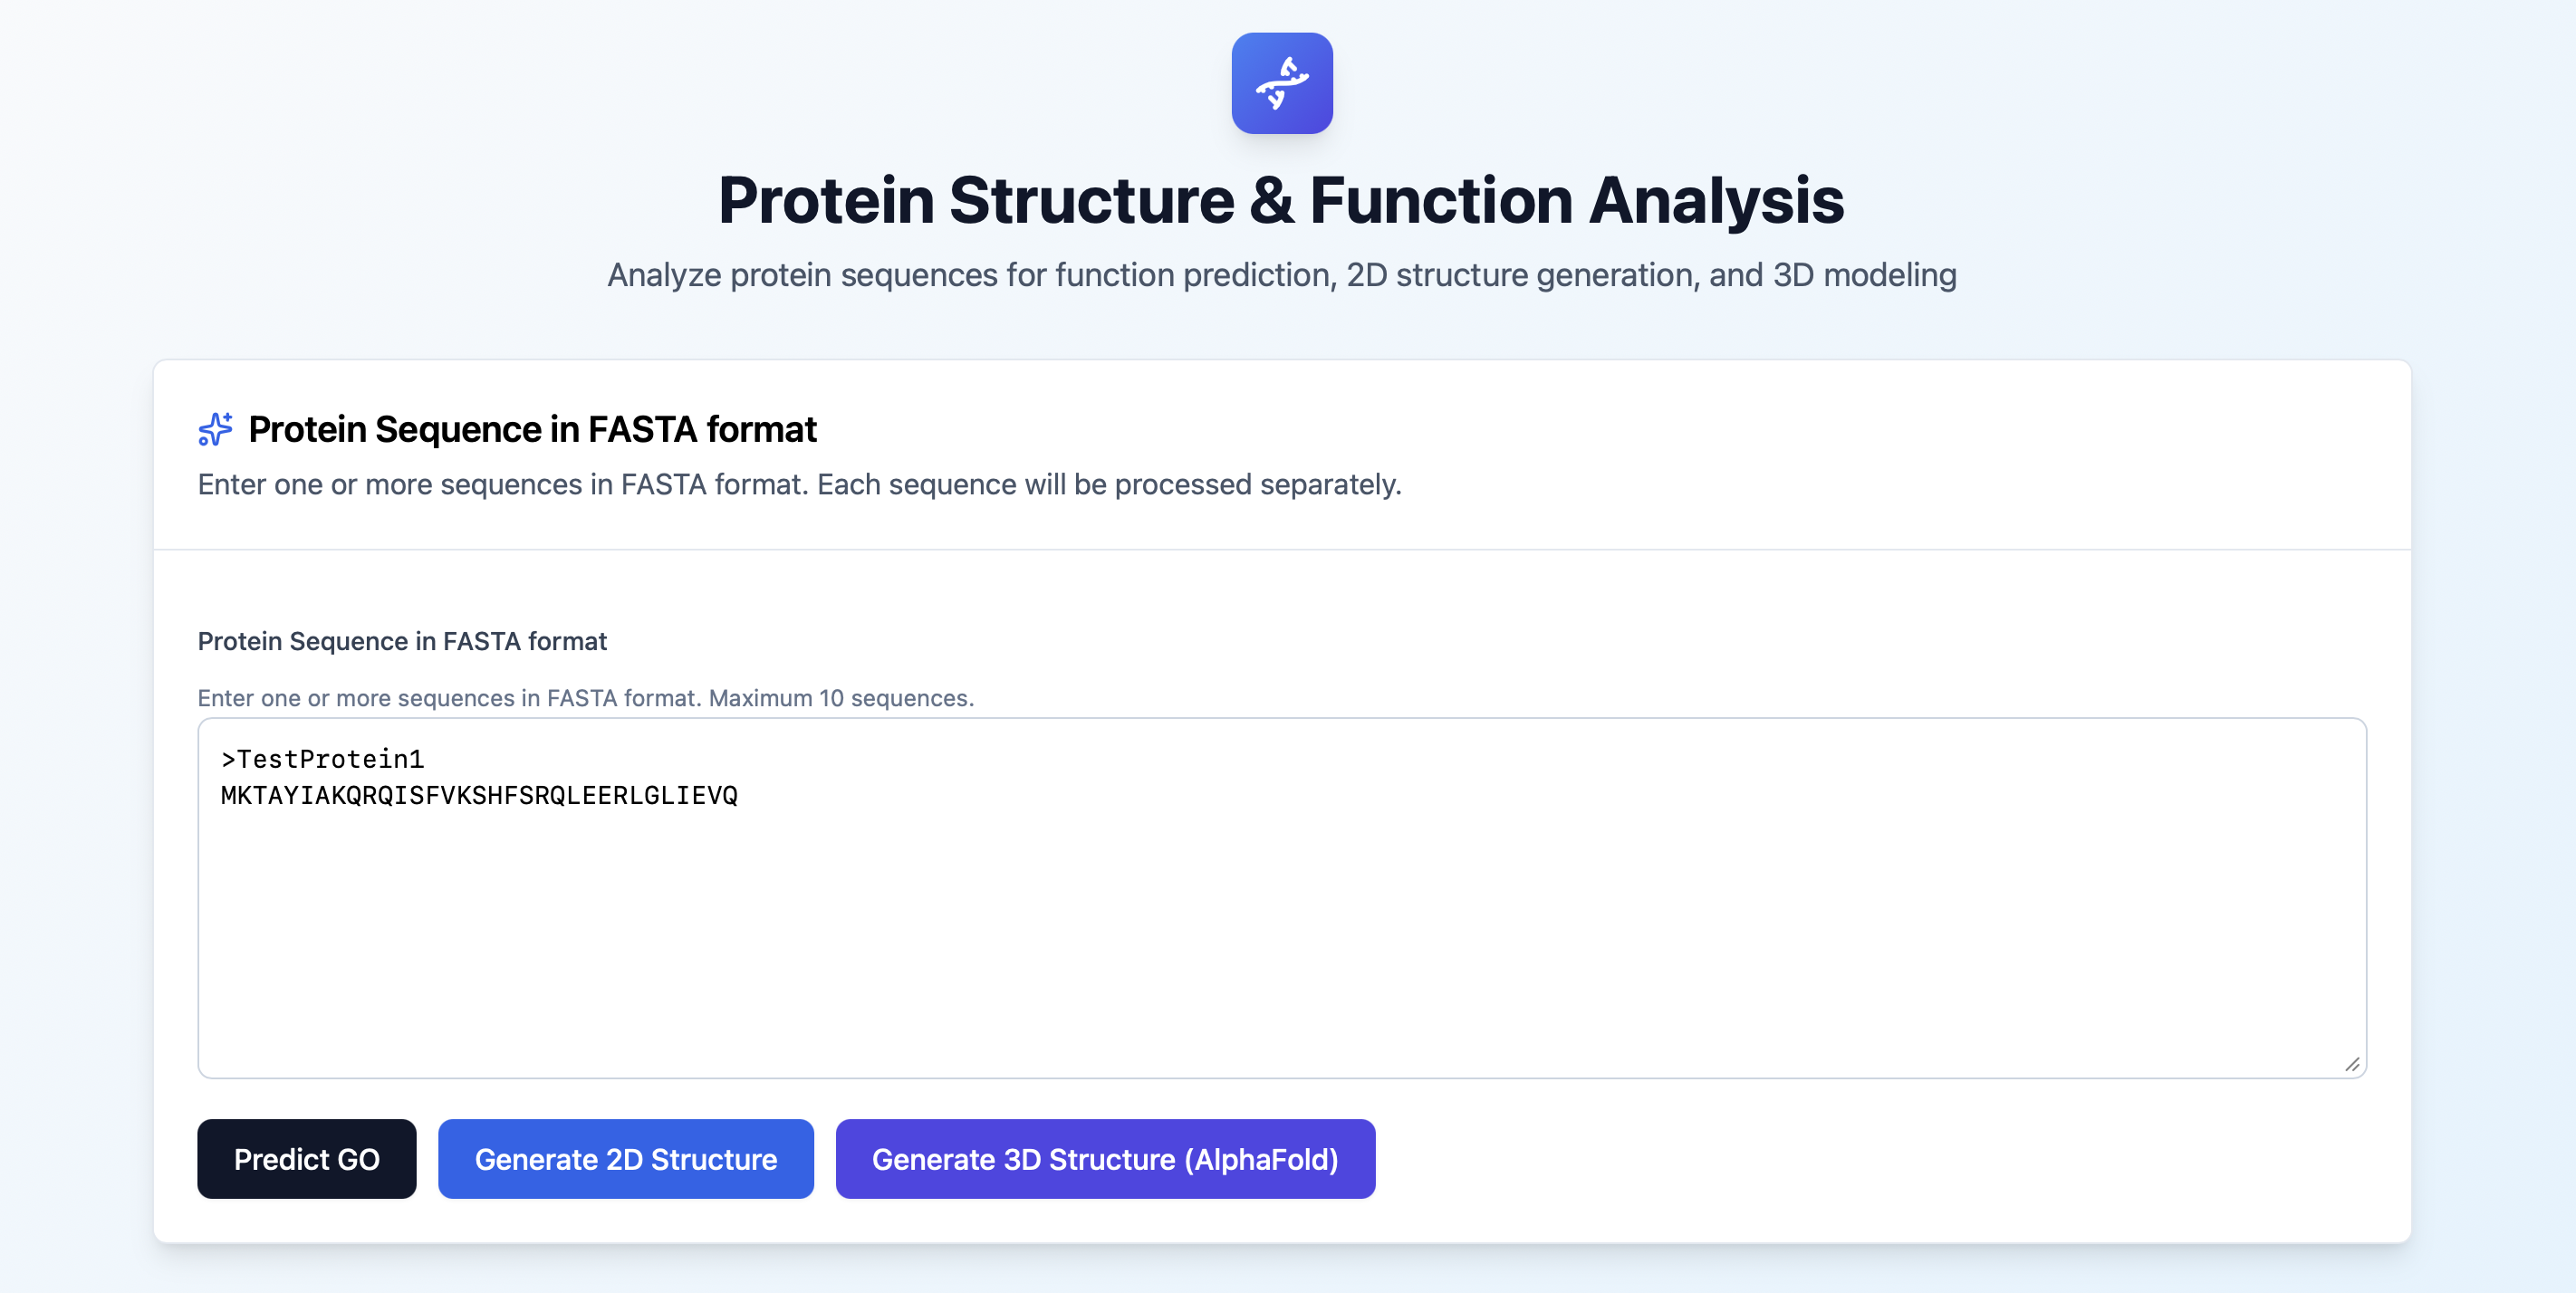
\includegraphics[width=\textwidth,height=0.76\textheight,keepaspectratio]{Figuras/proteinFastaInput.png}
\caption[FASTA input screen]{FASTA input screen of the web platform. Users can submit one or more protein sequences and choose between GO prediction, 2D HP folding, and 3D structure retrieval.}
\label{fig:appendix_fasta_input}
\end{figure}
\FloatBarrier

\begin{figure}[!htbp]
\centering
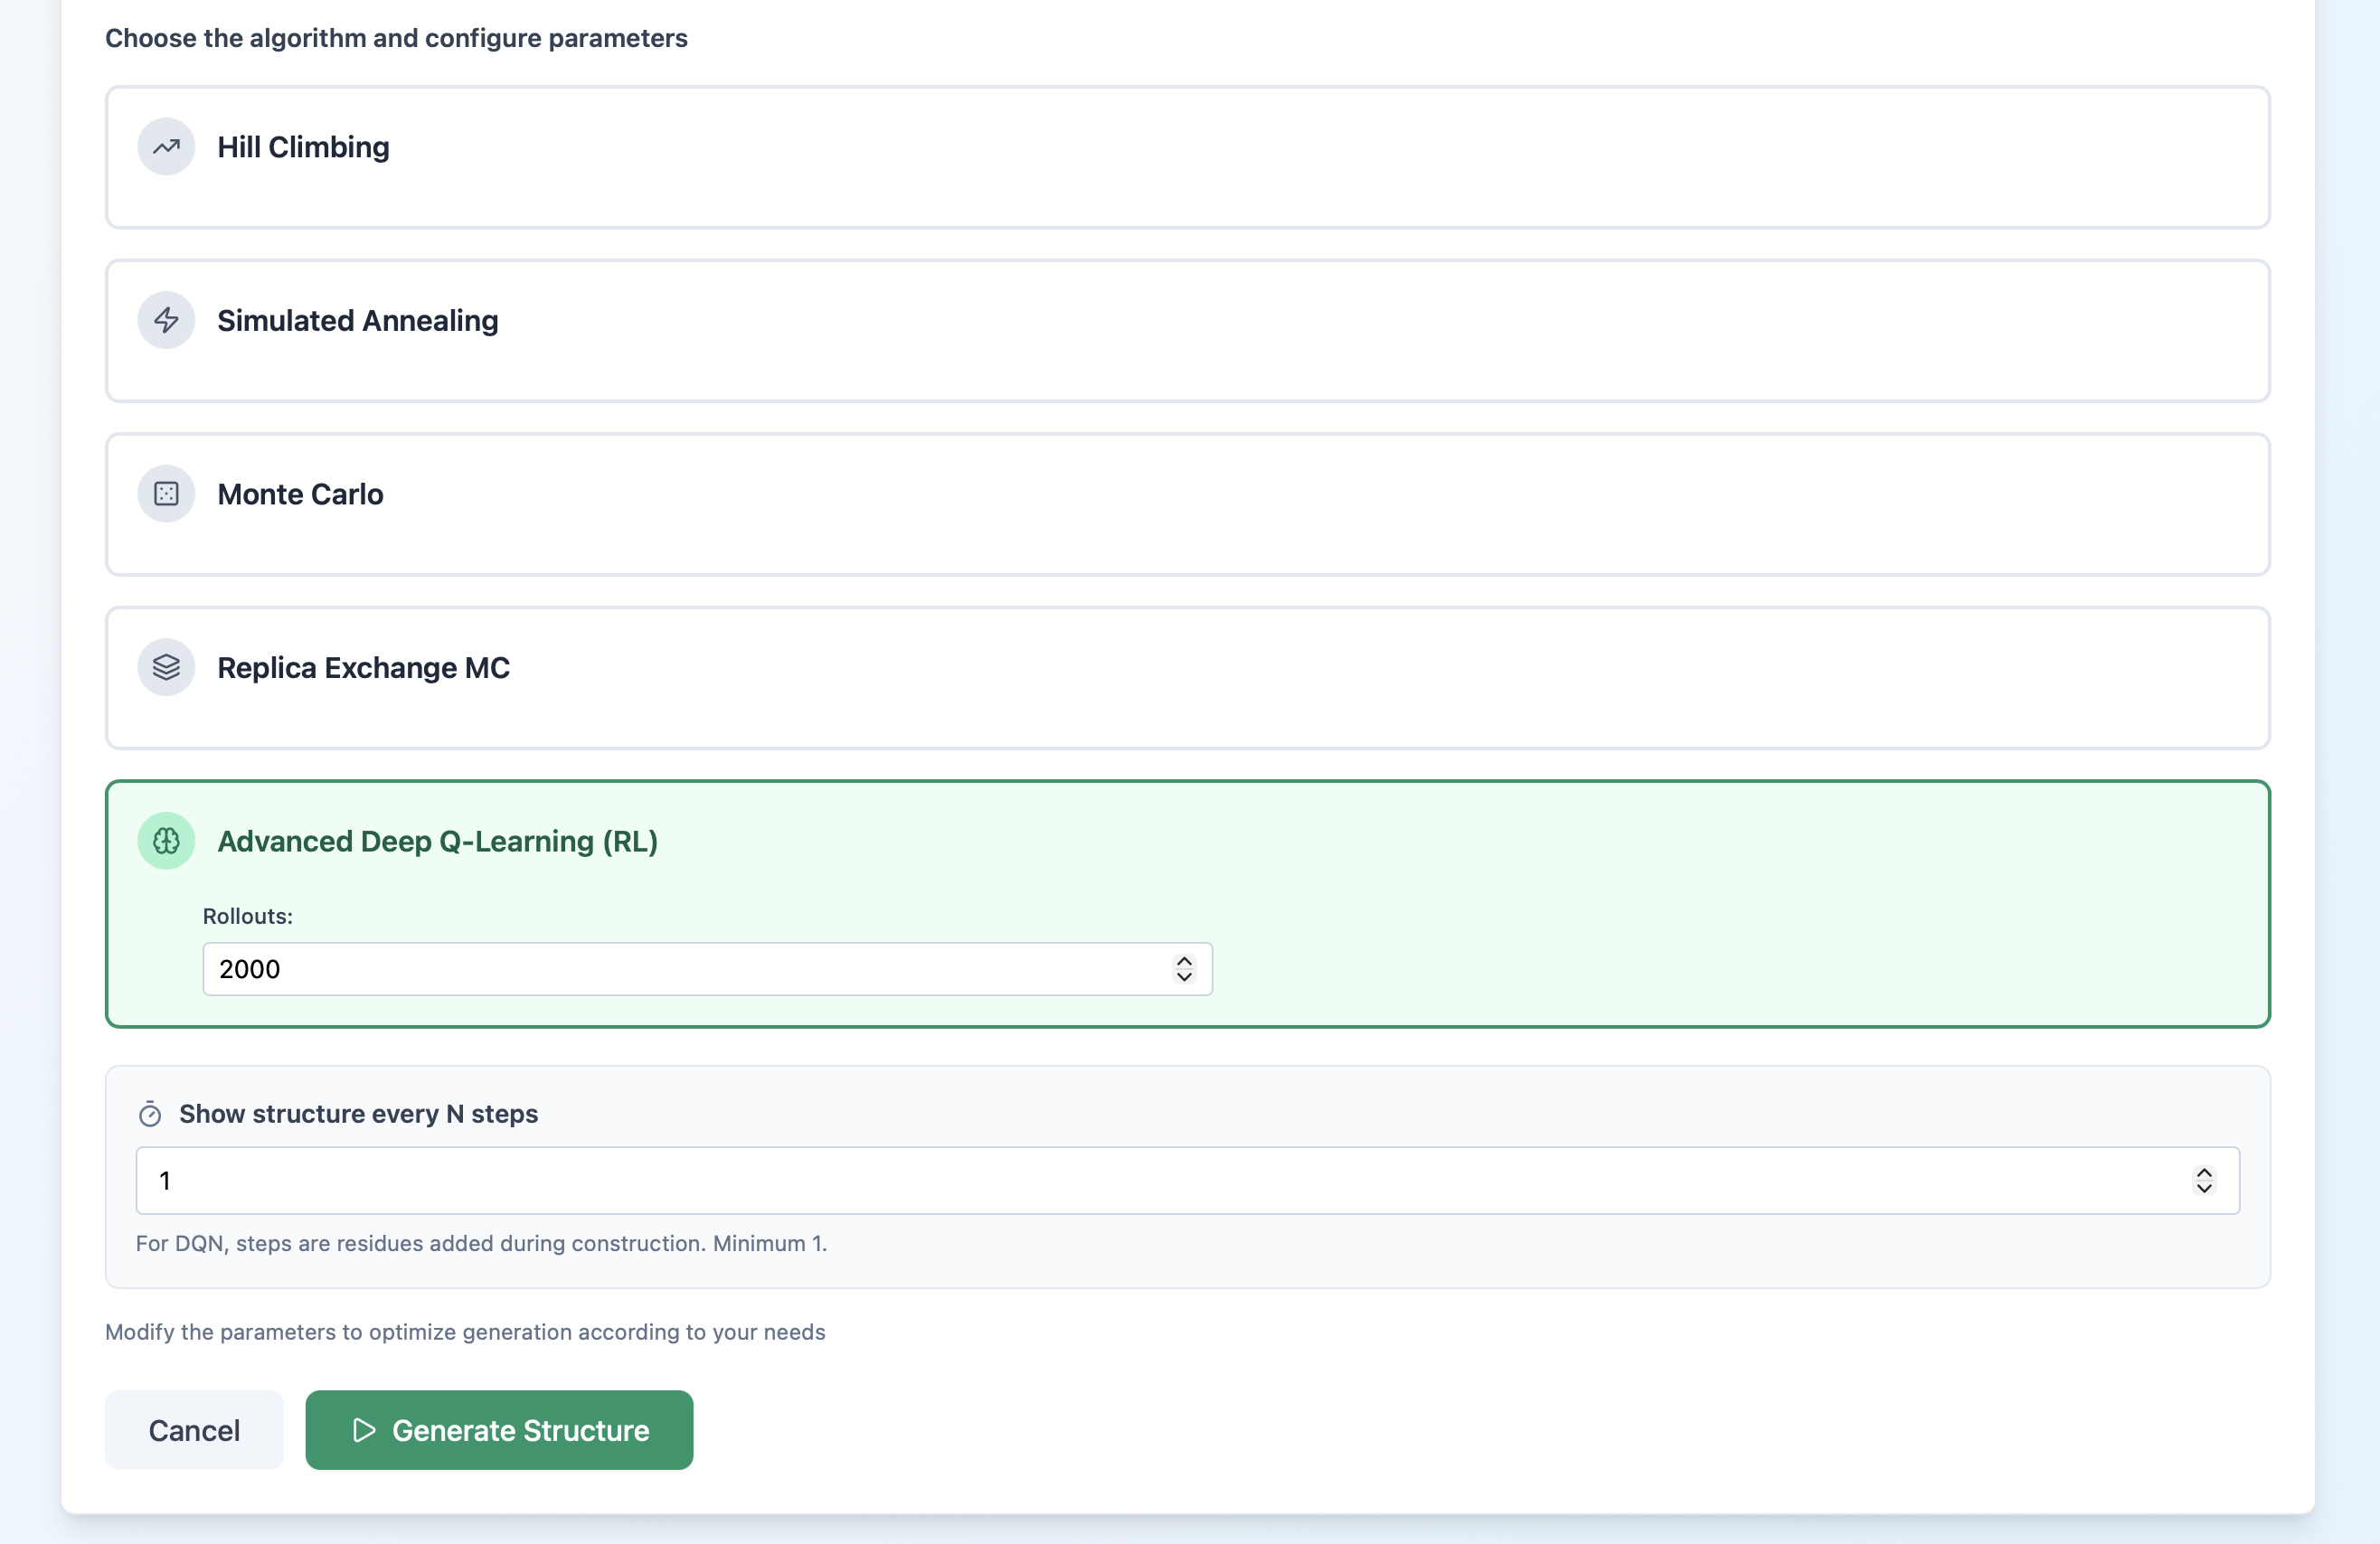
\includegraphics[width=\textwidth,height=0.76\textheight,keepaspectratio]{Figuras/algorithmSelection.png}
\caption[Algorithm selection screen]{Algorithm selection screen for 2D structure generation. The interface exposes the implemented optimization and reinforcement learning methods through a unified workflow. The selected DQN configuration shows the rollout parameter and the step-visualization interval, allowing users to choose how frequently intermediate conformations should be recorded and displayed.}
\label{fig:appendix_algorithm_selection}
\end{figure}
\FloatBarrier

\begin{figure}[!htbp]
\centering
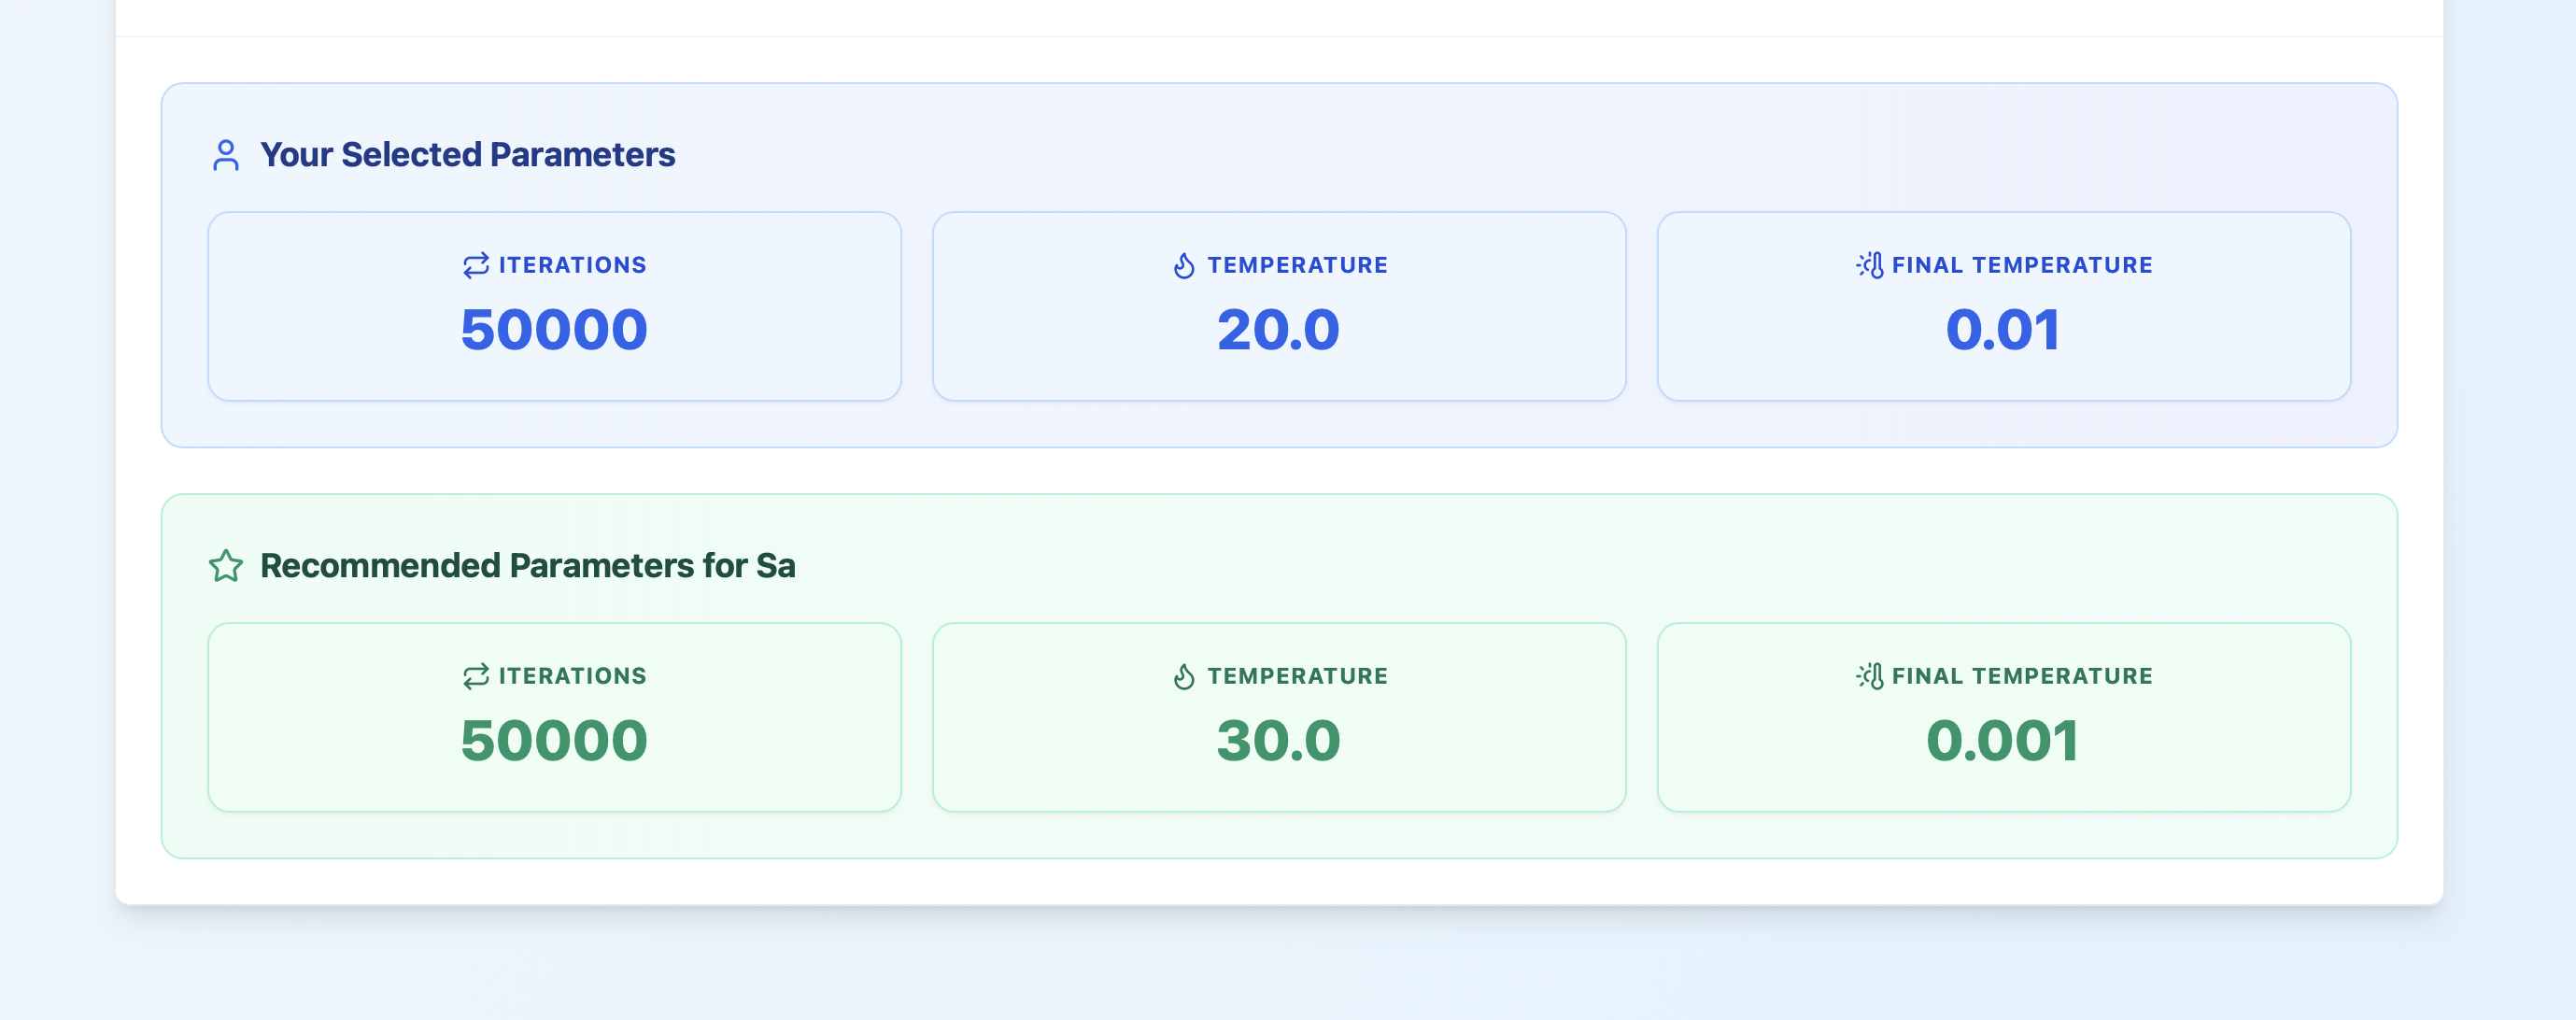
\includegraphics[width=\textwidth,height=0.76\textheight,keepaspectratio]{Figuras/2dStructureParam.png}
\caption[2D structure parameter panel]{Parameter configuration panel for 2D HP structure generation. Algorithm-specific controls allow users to tune iteration budgets, temperatures, replicas, learning parameters, and the interval used by the step explorer to display intermediate folding states.}
\label{fig:appendix_structure_parameters}
\end{figure}
\FloatBarrier
% !TEX root = ../main.tex


\newpage

% Anexo B
%--------------------------------------
% Obs#5
% Definir o título do anexo B
\newcommand{\tituloanexoB}{Web Platform Results}
%--------------------------------------
\phantomsection
\addcontentsline{toc}{section}{Anexo B - \tituloanexoB}

% Anexo
%--------------------------------------
\vspace*{45pt}
% Título do anexo B (\tituloanexoB) definido no ficheiro main
\section*{Anexo B - \tituloanexoB}

This appendix presents representative output screens produced by the web platform, including Gene Ontology prediction, 2D HP lattice visualization with step-by-step exploration, and interactive 3D structure retrieval.

\begin{figure}[!htbp]
\centering
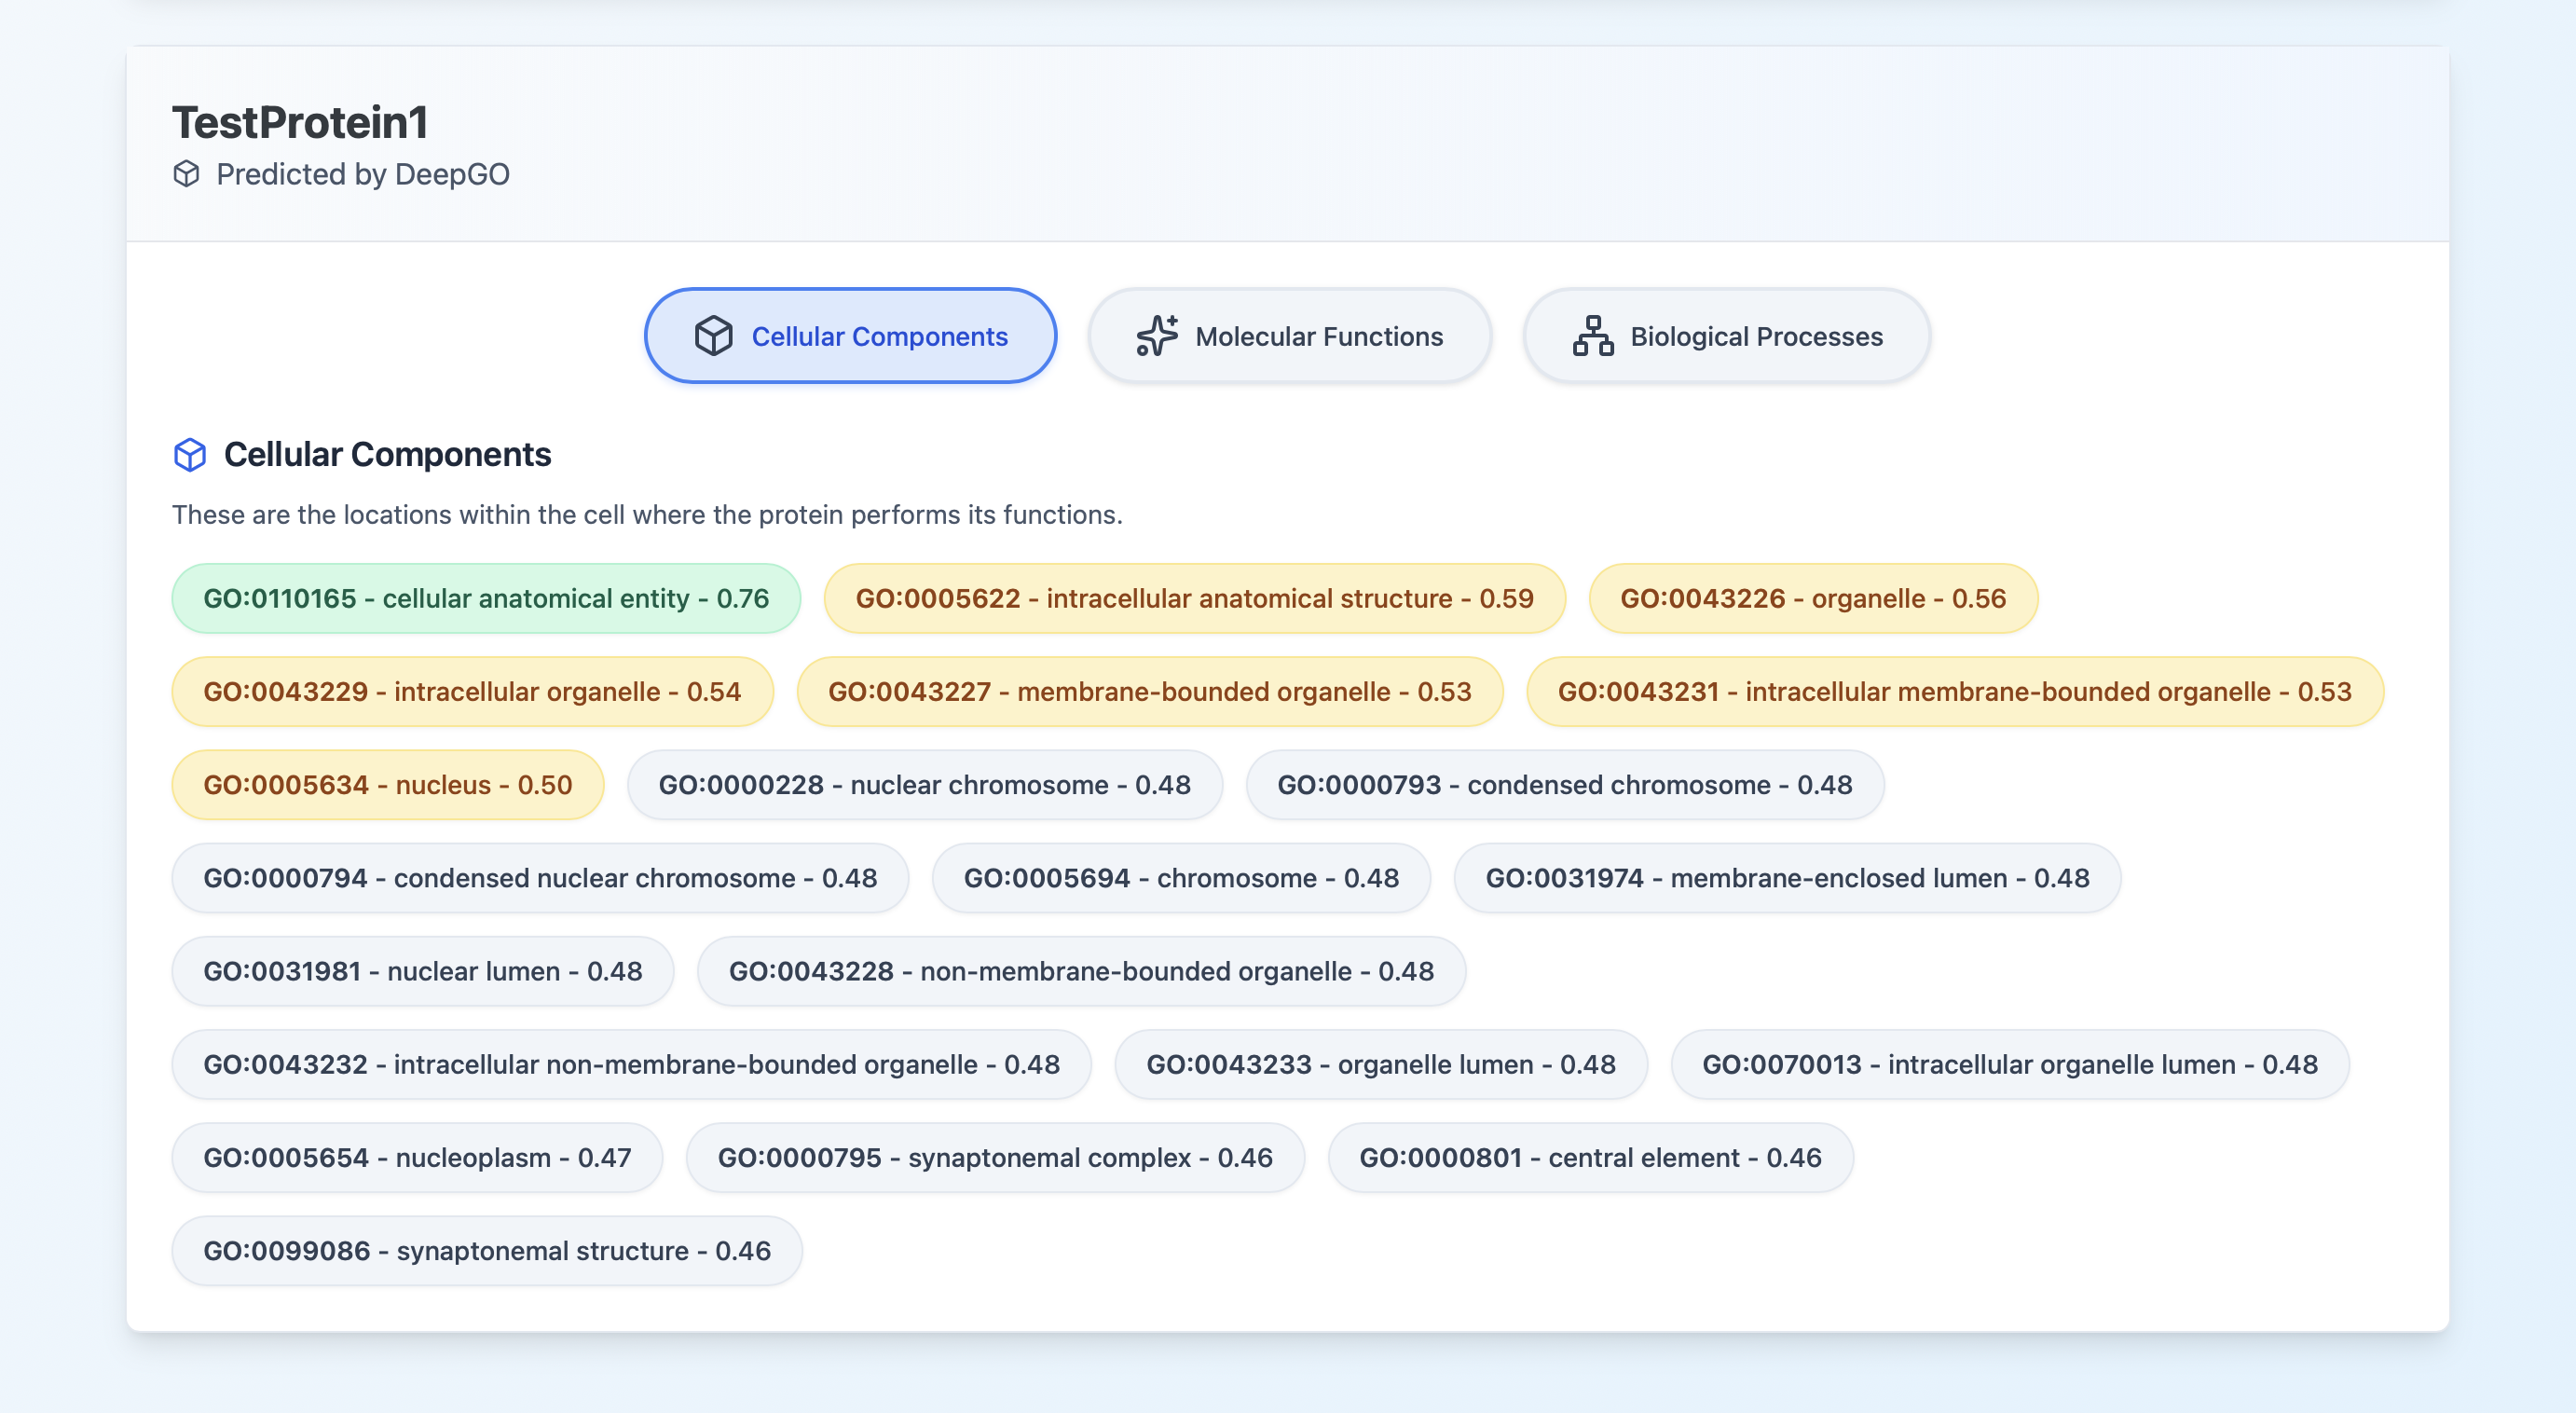
\includegraphics[width=\textwidth,height=0.76\textheight,keepaspectratio]{Figuras/goTermsResult.png}
\caption[GO prediction results screen]{GO prediction results screen. Predicted Gene Ontology terms are grouped by biological process, molecular function, and cellular component when returned by the external DeepGO service.}
\label{fig:appendix_go_results}
\end{figure}
\FloatBarrier

Figures~\ref{fig:appendix_2d_structure_step_initial}--\ref{fig:appendix_2d_structure_step_final} illustrate the step explorer added to the 2D structure visualization workflow. Instead of showing only the final conformation, the platform stores intermediate frames according to the user-defined interval and lets the user navigate the folding trajectory with previous, play, next, and slider controls. For the constructive DQN, each displayed step corresponds to one or more residues added during chain construction; for classical algorithms, each displayed step corresponds to a sampled optimization interval.

In the deployed web version, the number of DQN rollouts was scaled down due to the limited computational resources of the hosting environment.

\begin{figure}[!htbp]
\centering
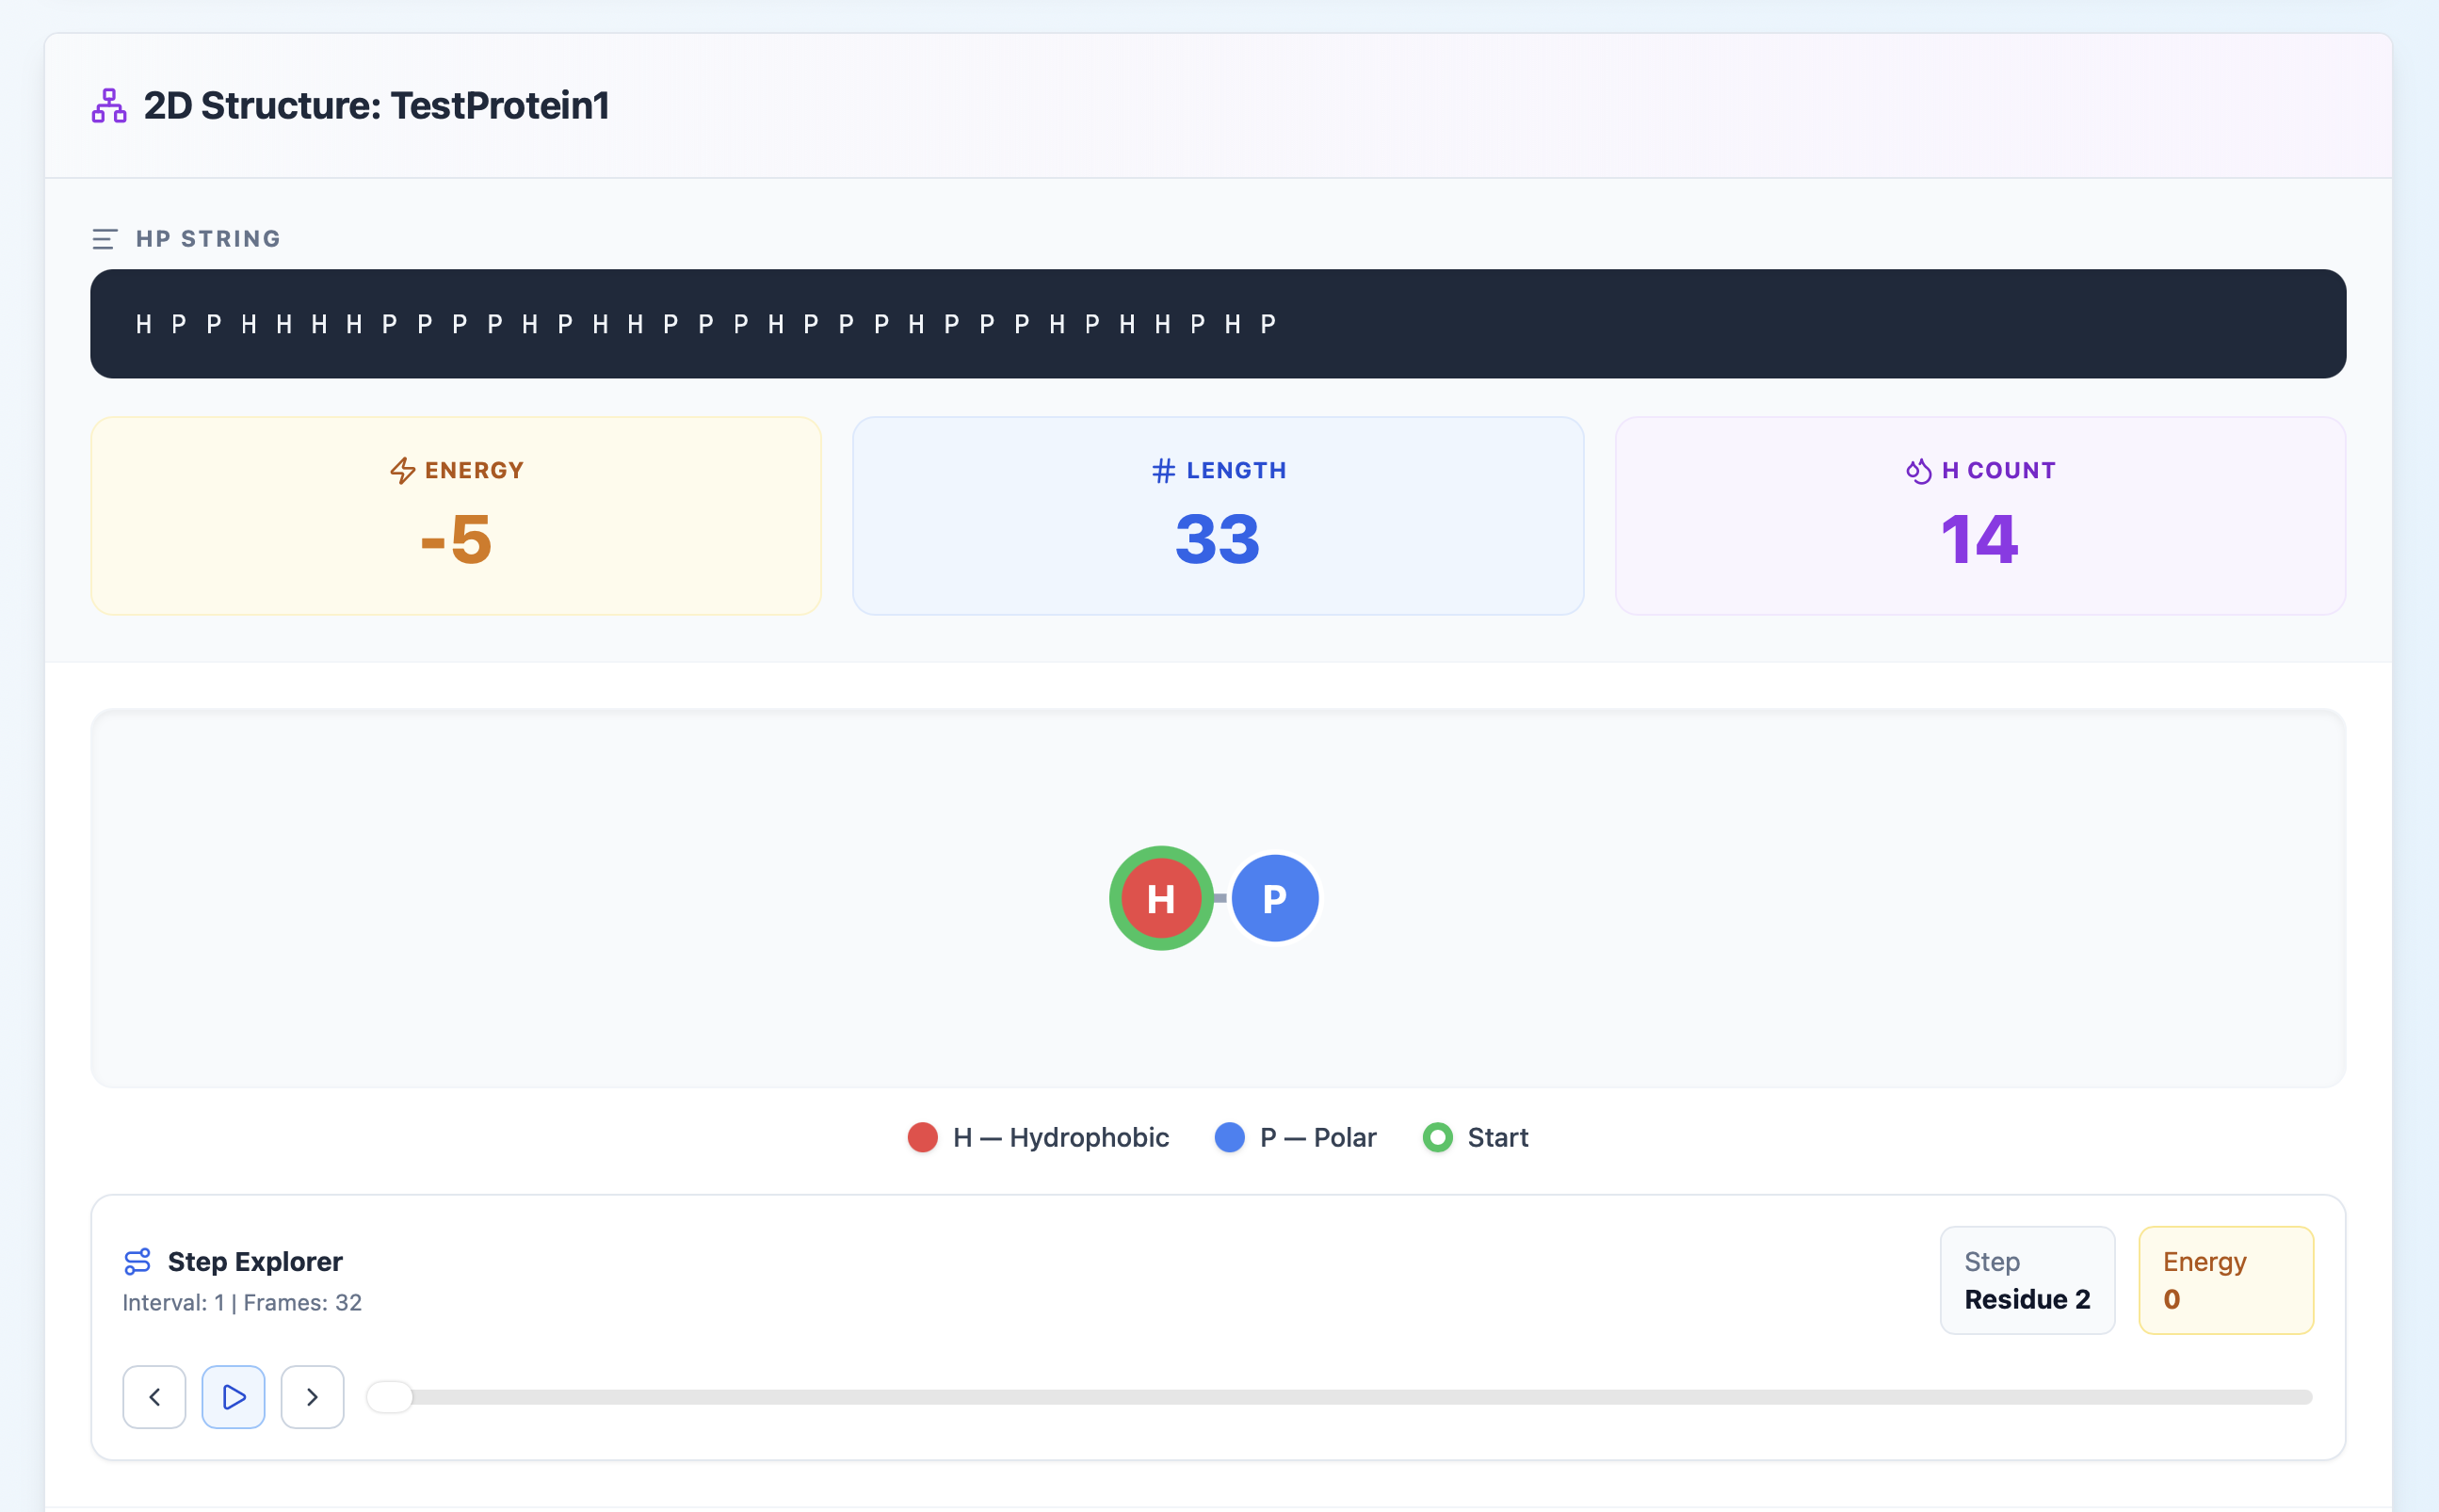
\includegraphics[width=\textwidth,height=0.70\textheight,keepaspectratio]{Figuras/2dStructure.png}
\caption[2D HP step explorer: initial frame]{Initial 2D HP step-explorer frame. The protein construction starts from the first residues, with the current step, energy, frame count, and playback controls displayed below the SVG lattice.}
\label{fig:appendix_2d_structure_step_initial}
\end{figure}
\FloatBarrier

\begin{figure}[!htbp]
\centering
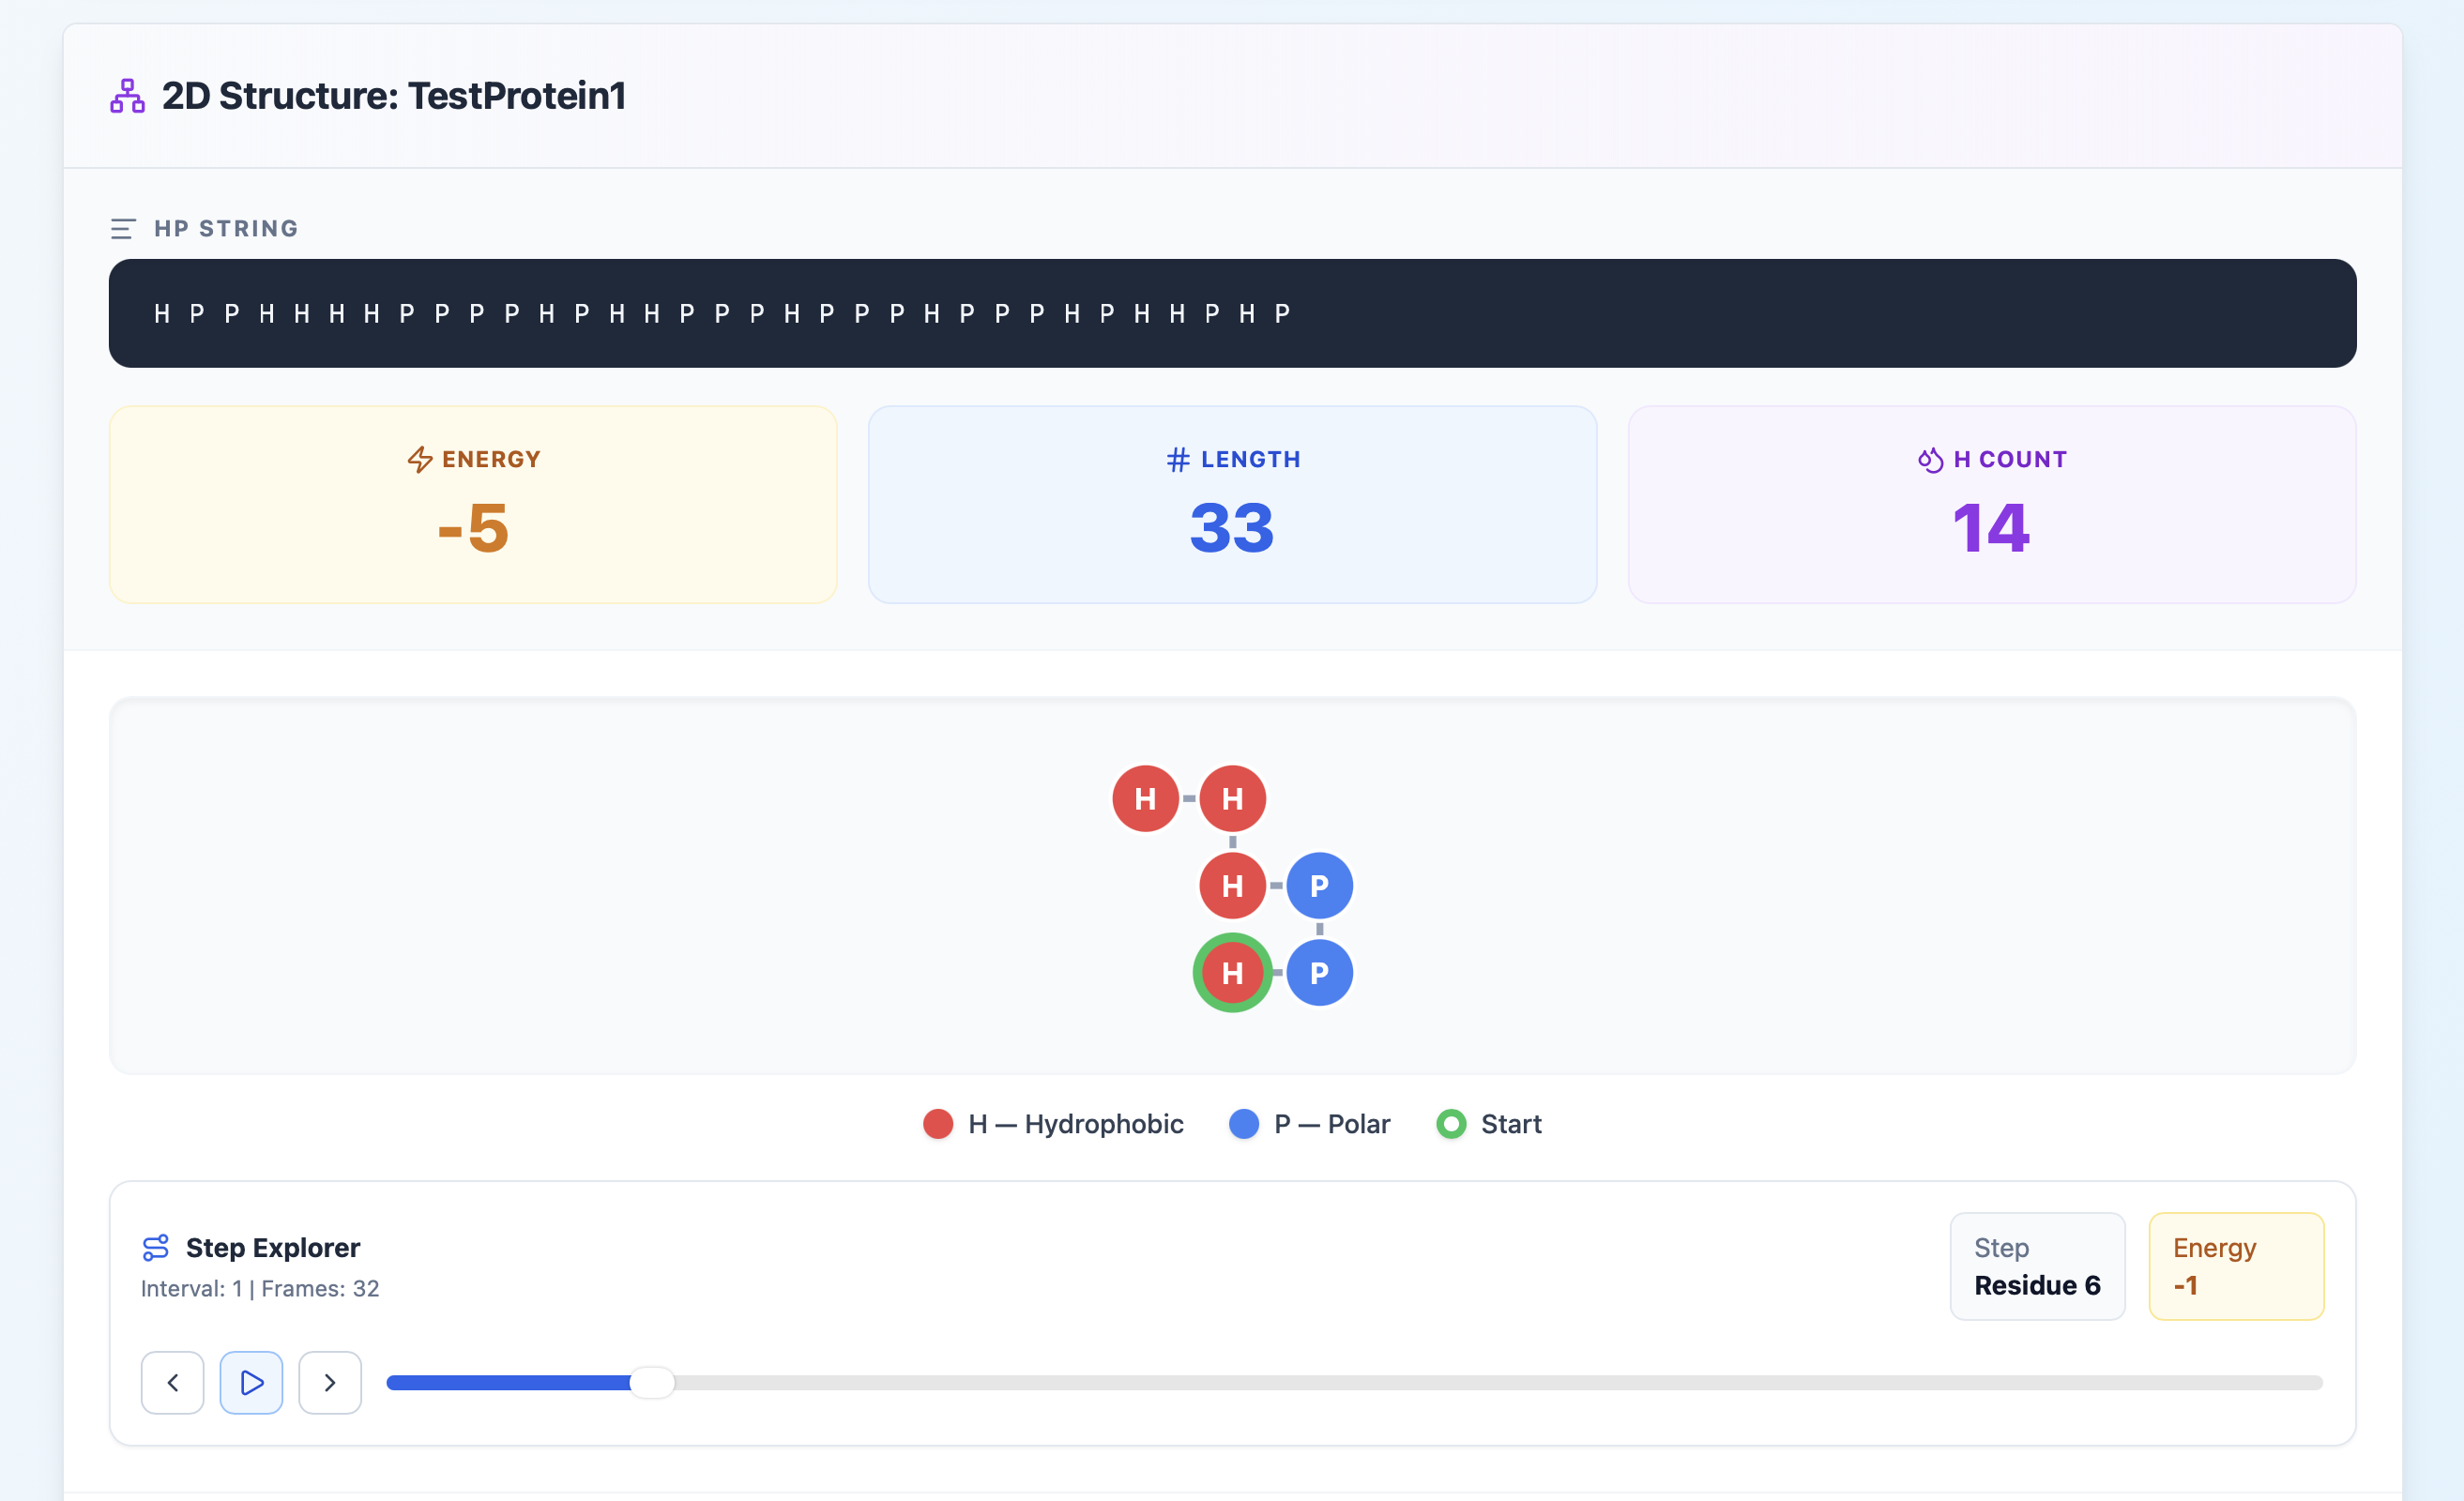
\includegraphics[width=\textwidth,height=0.70\textheight,keepaspectratio]{Figuras/2dStructure2.png}
\caption[2D HP step explorer: early folding frame]{Early folding frame in the 2D HP step explorer. The interface shows how the partial chain grows while preserving the same energy, sequence, and navigation context.}
\label{fig:appendix_2d_structure_step_early}
\end{figure}
\FloatBarrier

\begin{figure}[!htbp]
\centering
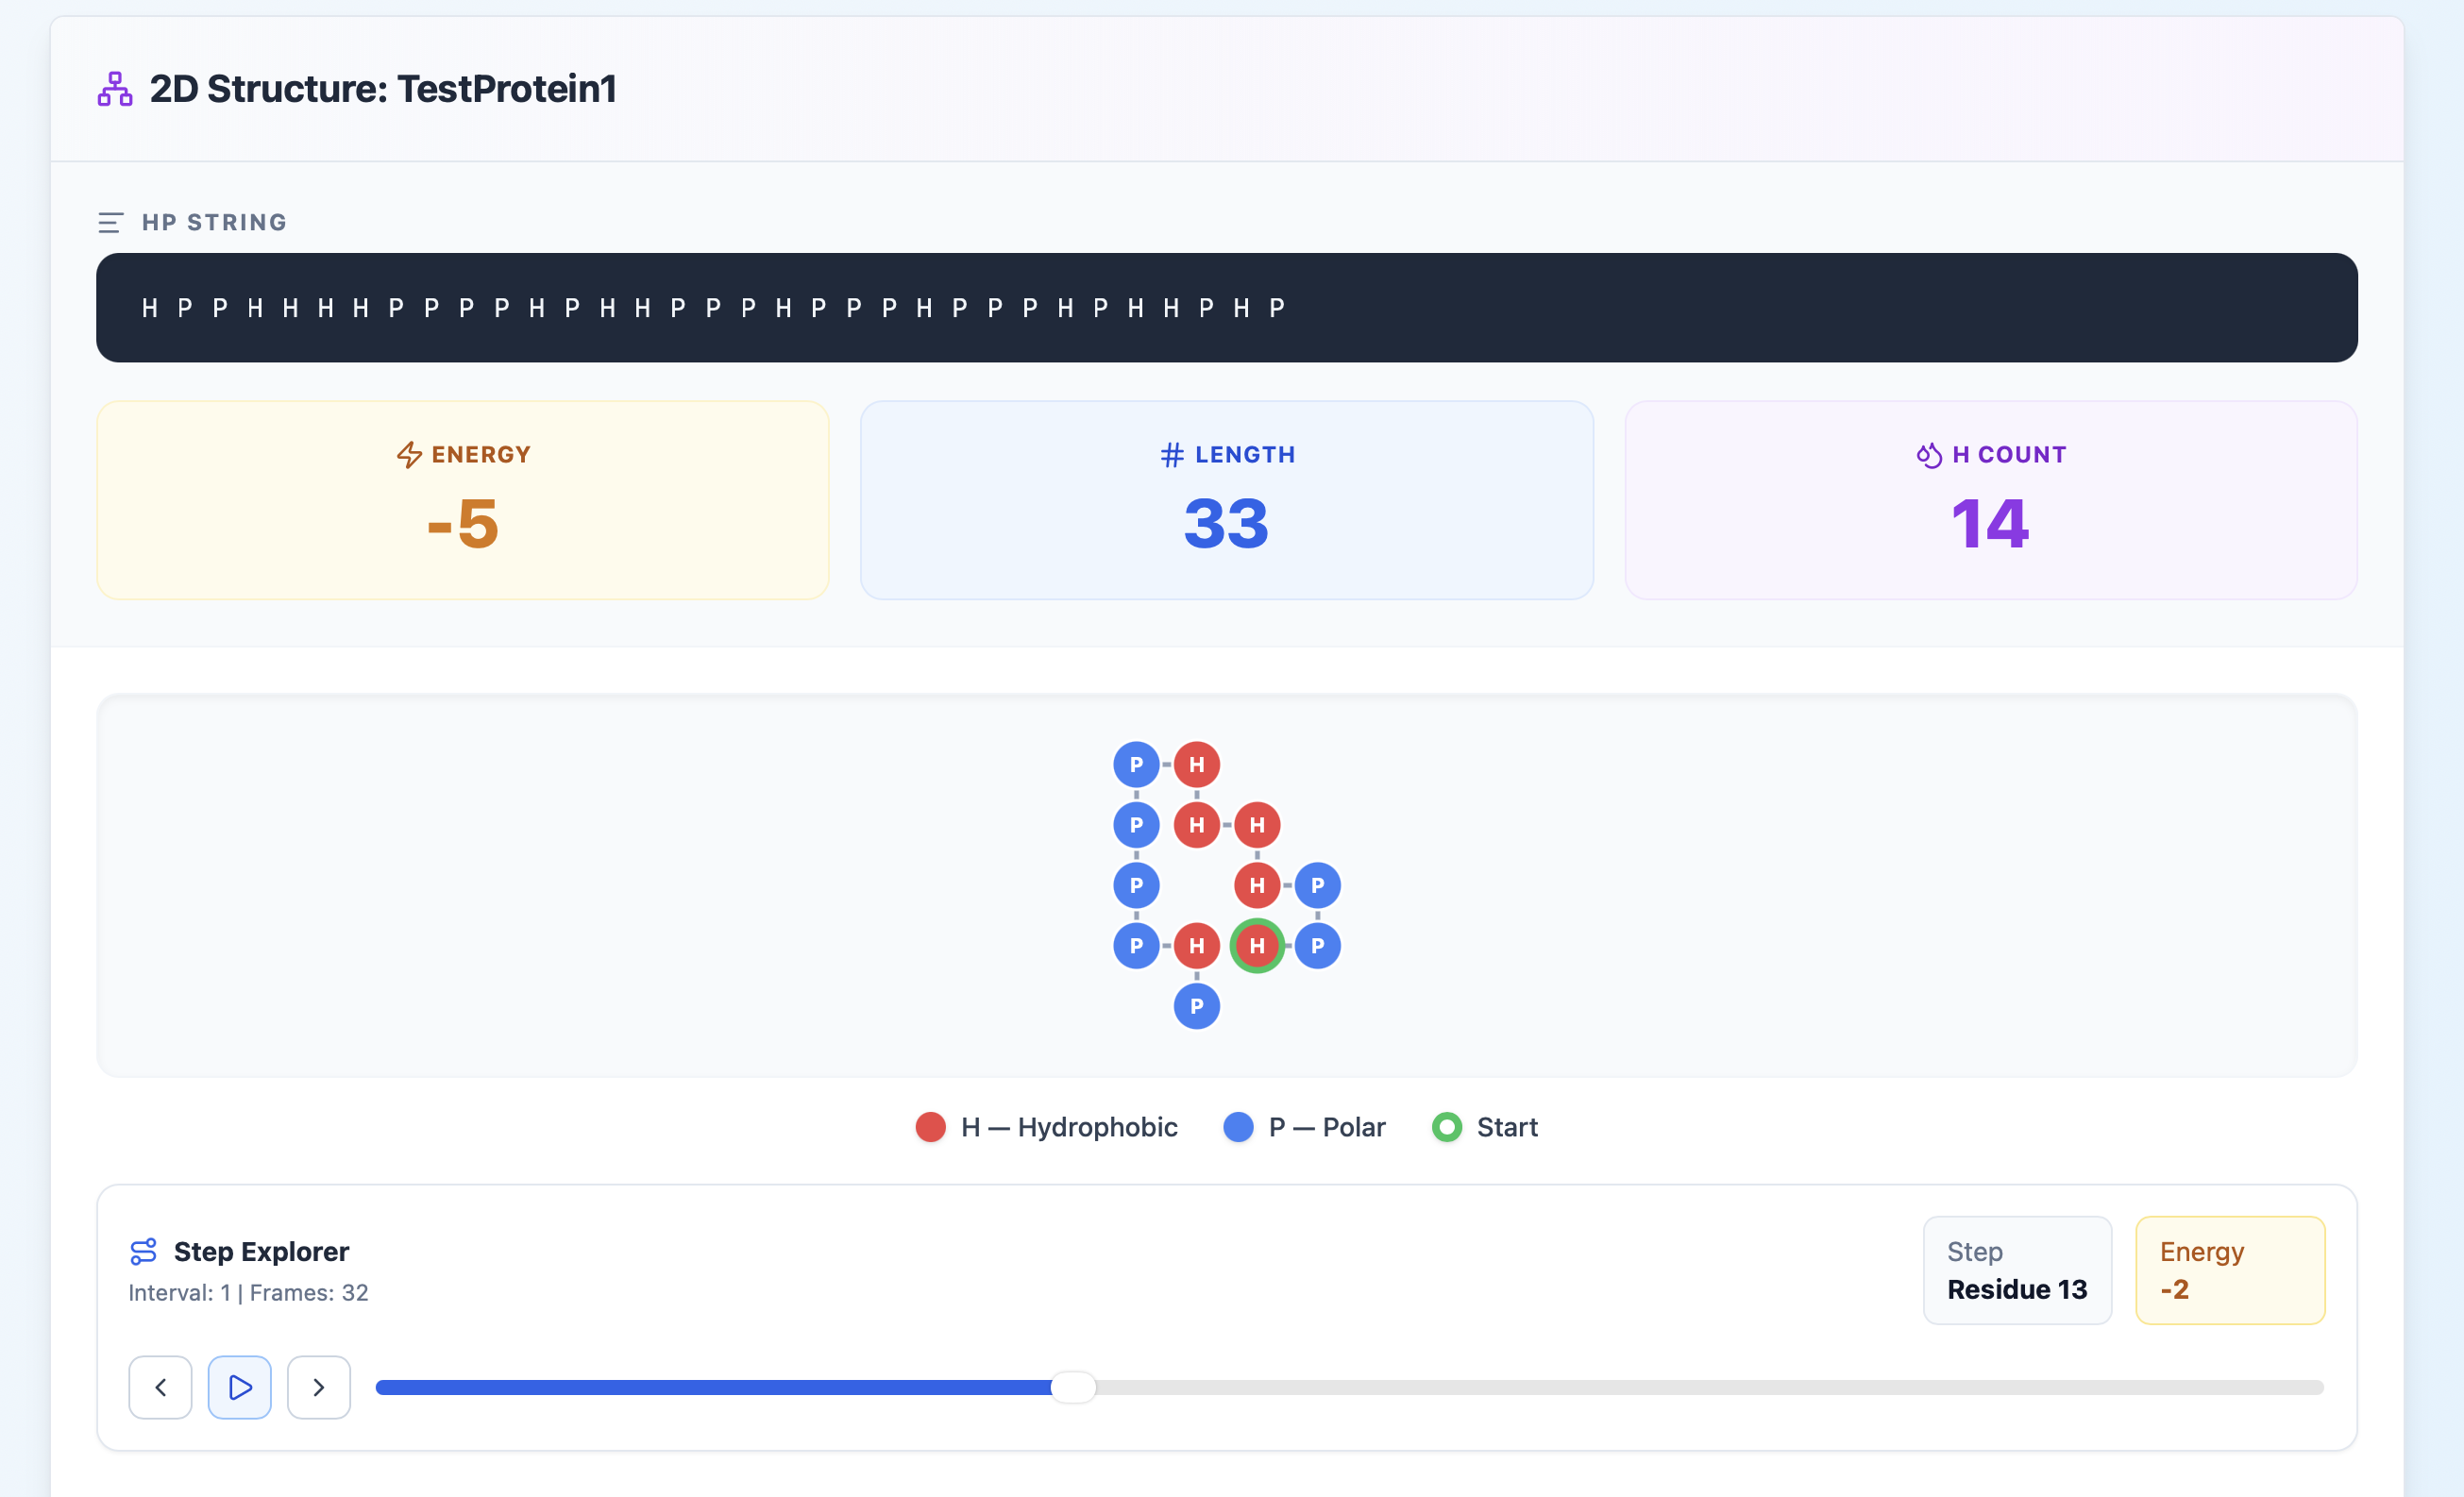
\includegraphics[width=\textwidth,height=0.70\textheight,keepaspectratio]{Figuras/2dStructure3.png}
\caption[2D HP step explorer: intermediate folding frame]{Intermediate folding frame in the 2D HP step explorer. The visualization makes it possible to inspect how local turns and hydrophobic contacts emerge before the final conformation is reached.}
\label{fig:appendix_2d_structure_step_intermediate}
\end{figure}
\FloatBarrier

\begin{figure}[!htbp]
\centering
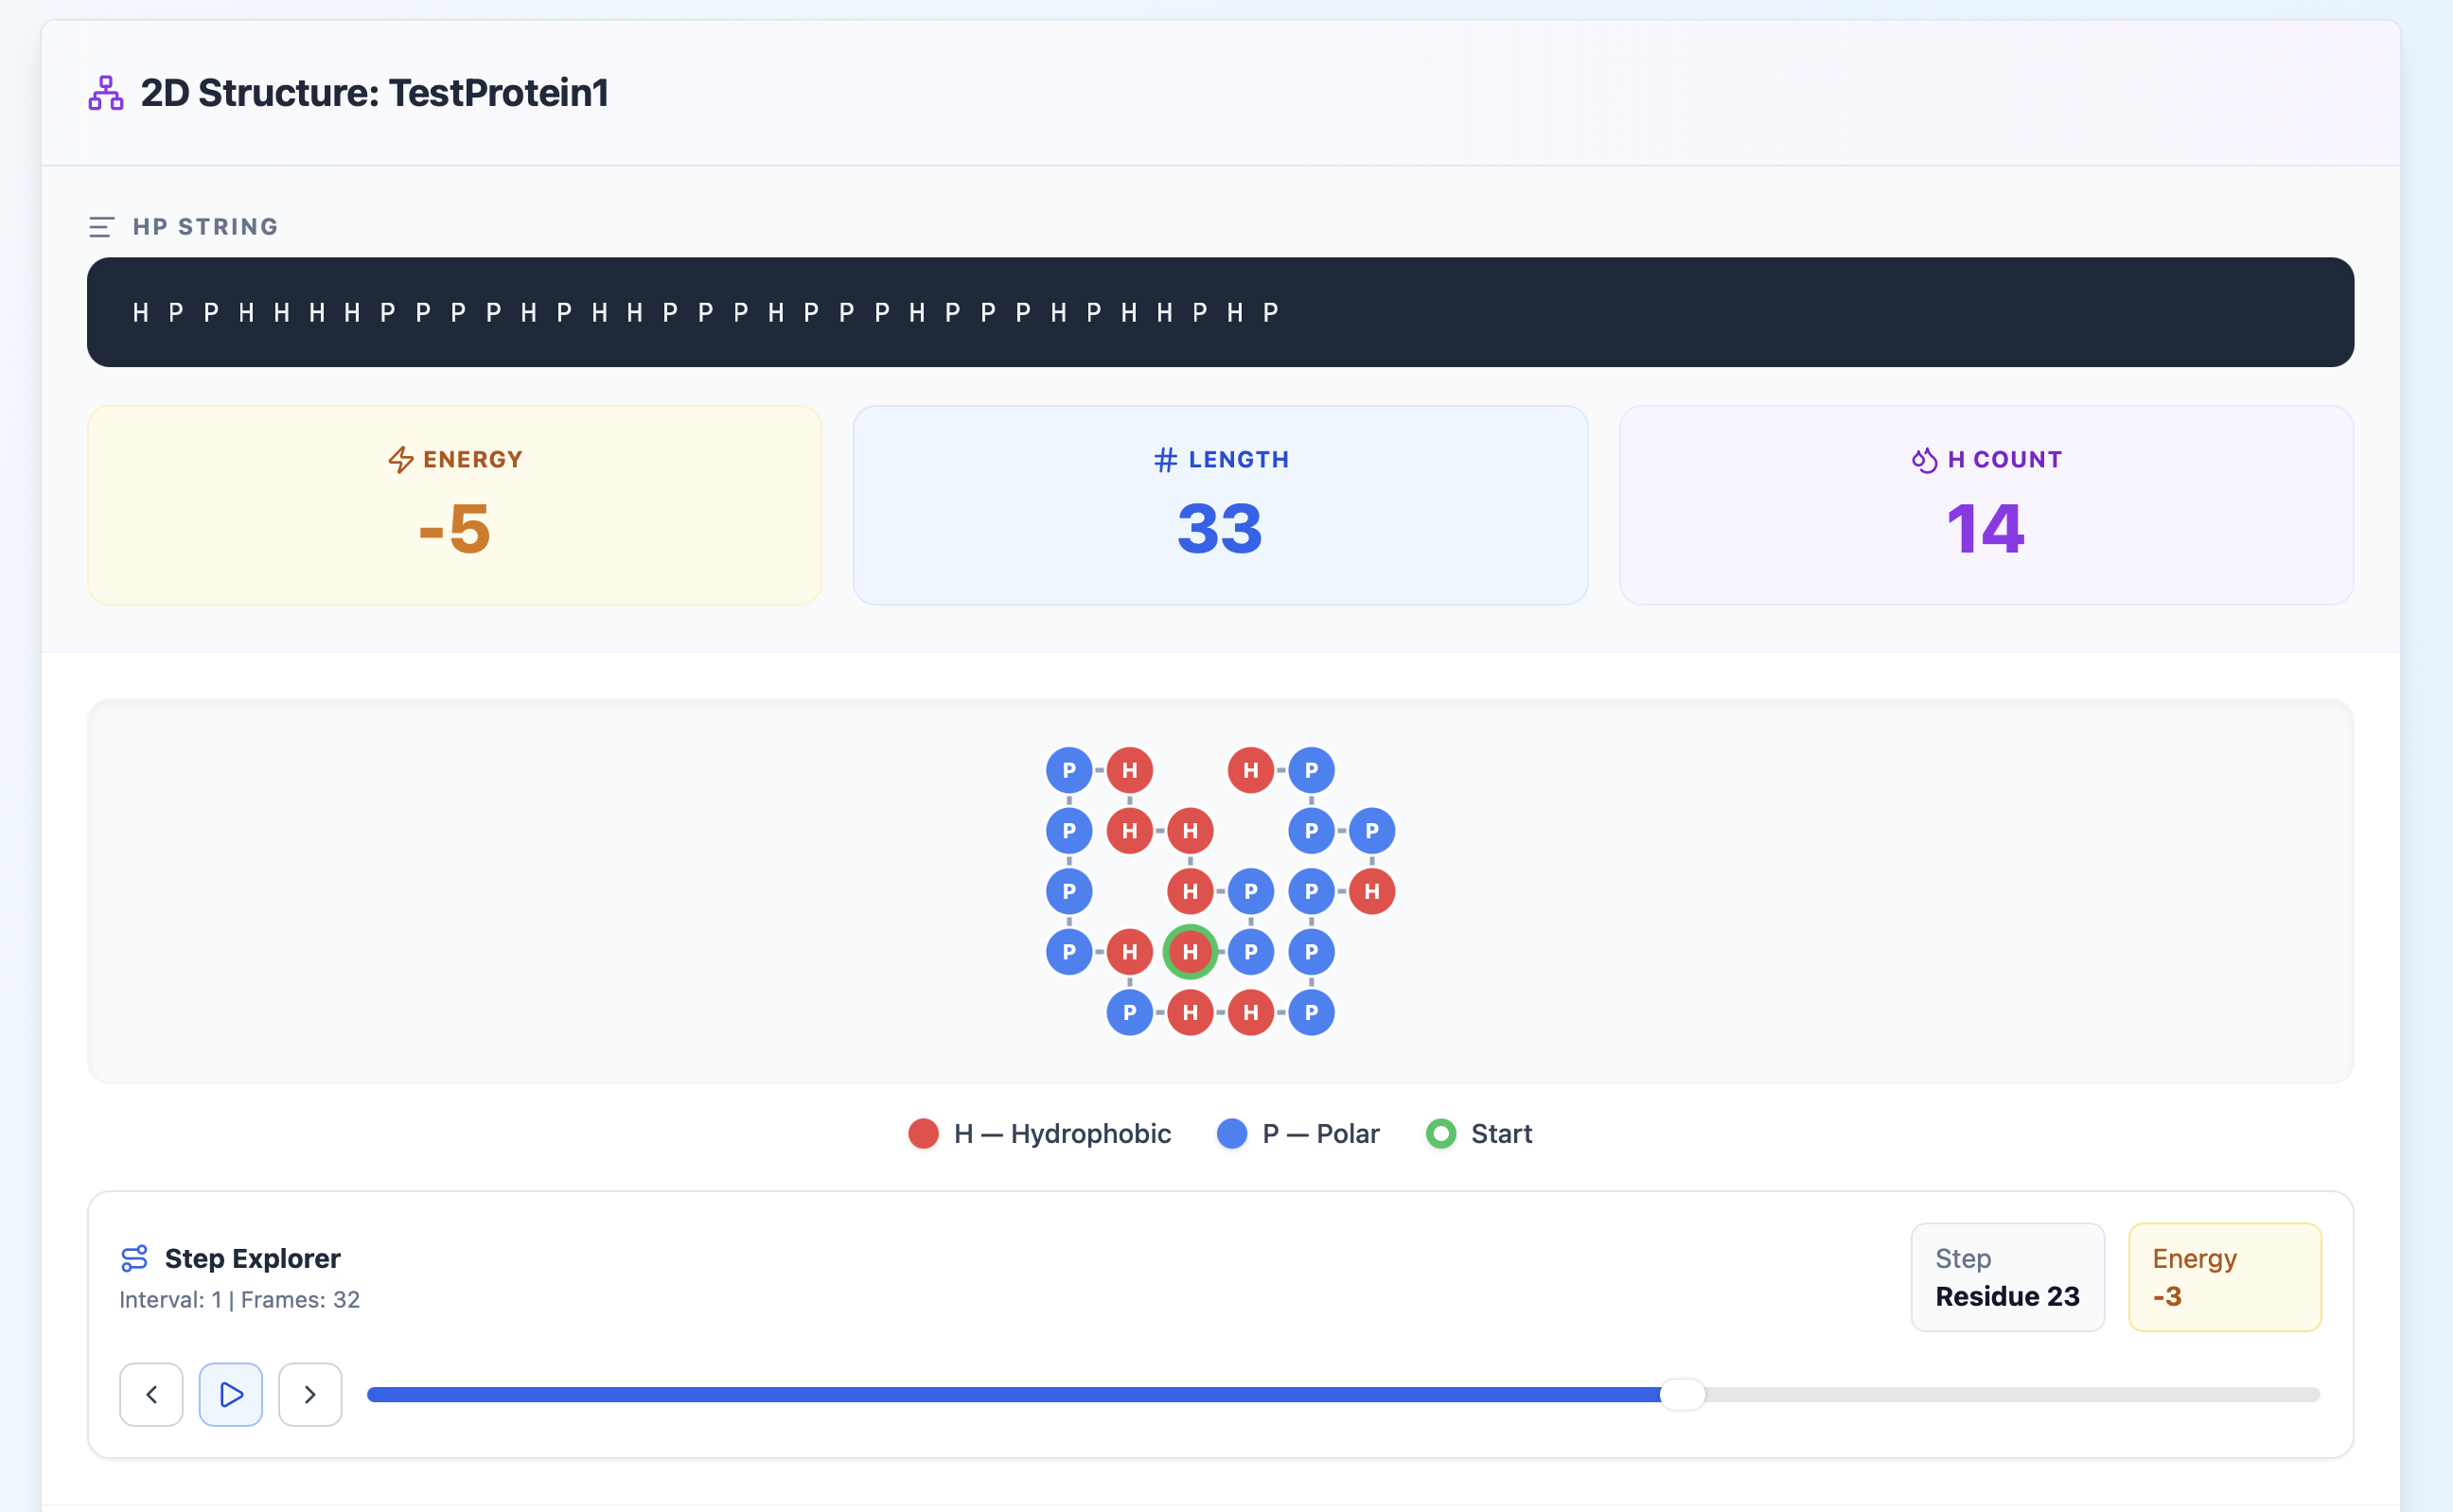
\includegraphics[width=\textwidth,height=0.70\textheight,keepaspectratio]{Figuras/2dStructure4.png}
\caption[2D HP step explorer: late folding frame]{Late folding frame in the 2D HP step explorer. The slider position and step counter allow the user to compare this near-final state with earlier conformations.}
\label{fig:appendix_2d_structure_step_late}
\end{figure}
\FloatBarrier

\begin{figure}[!htbp]
\centering
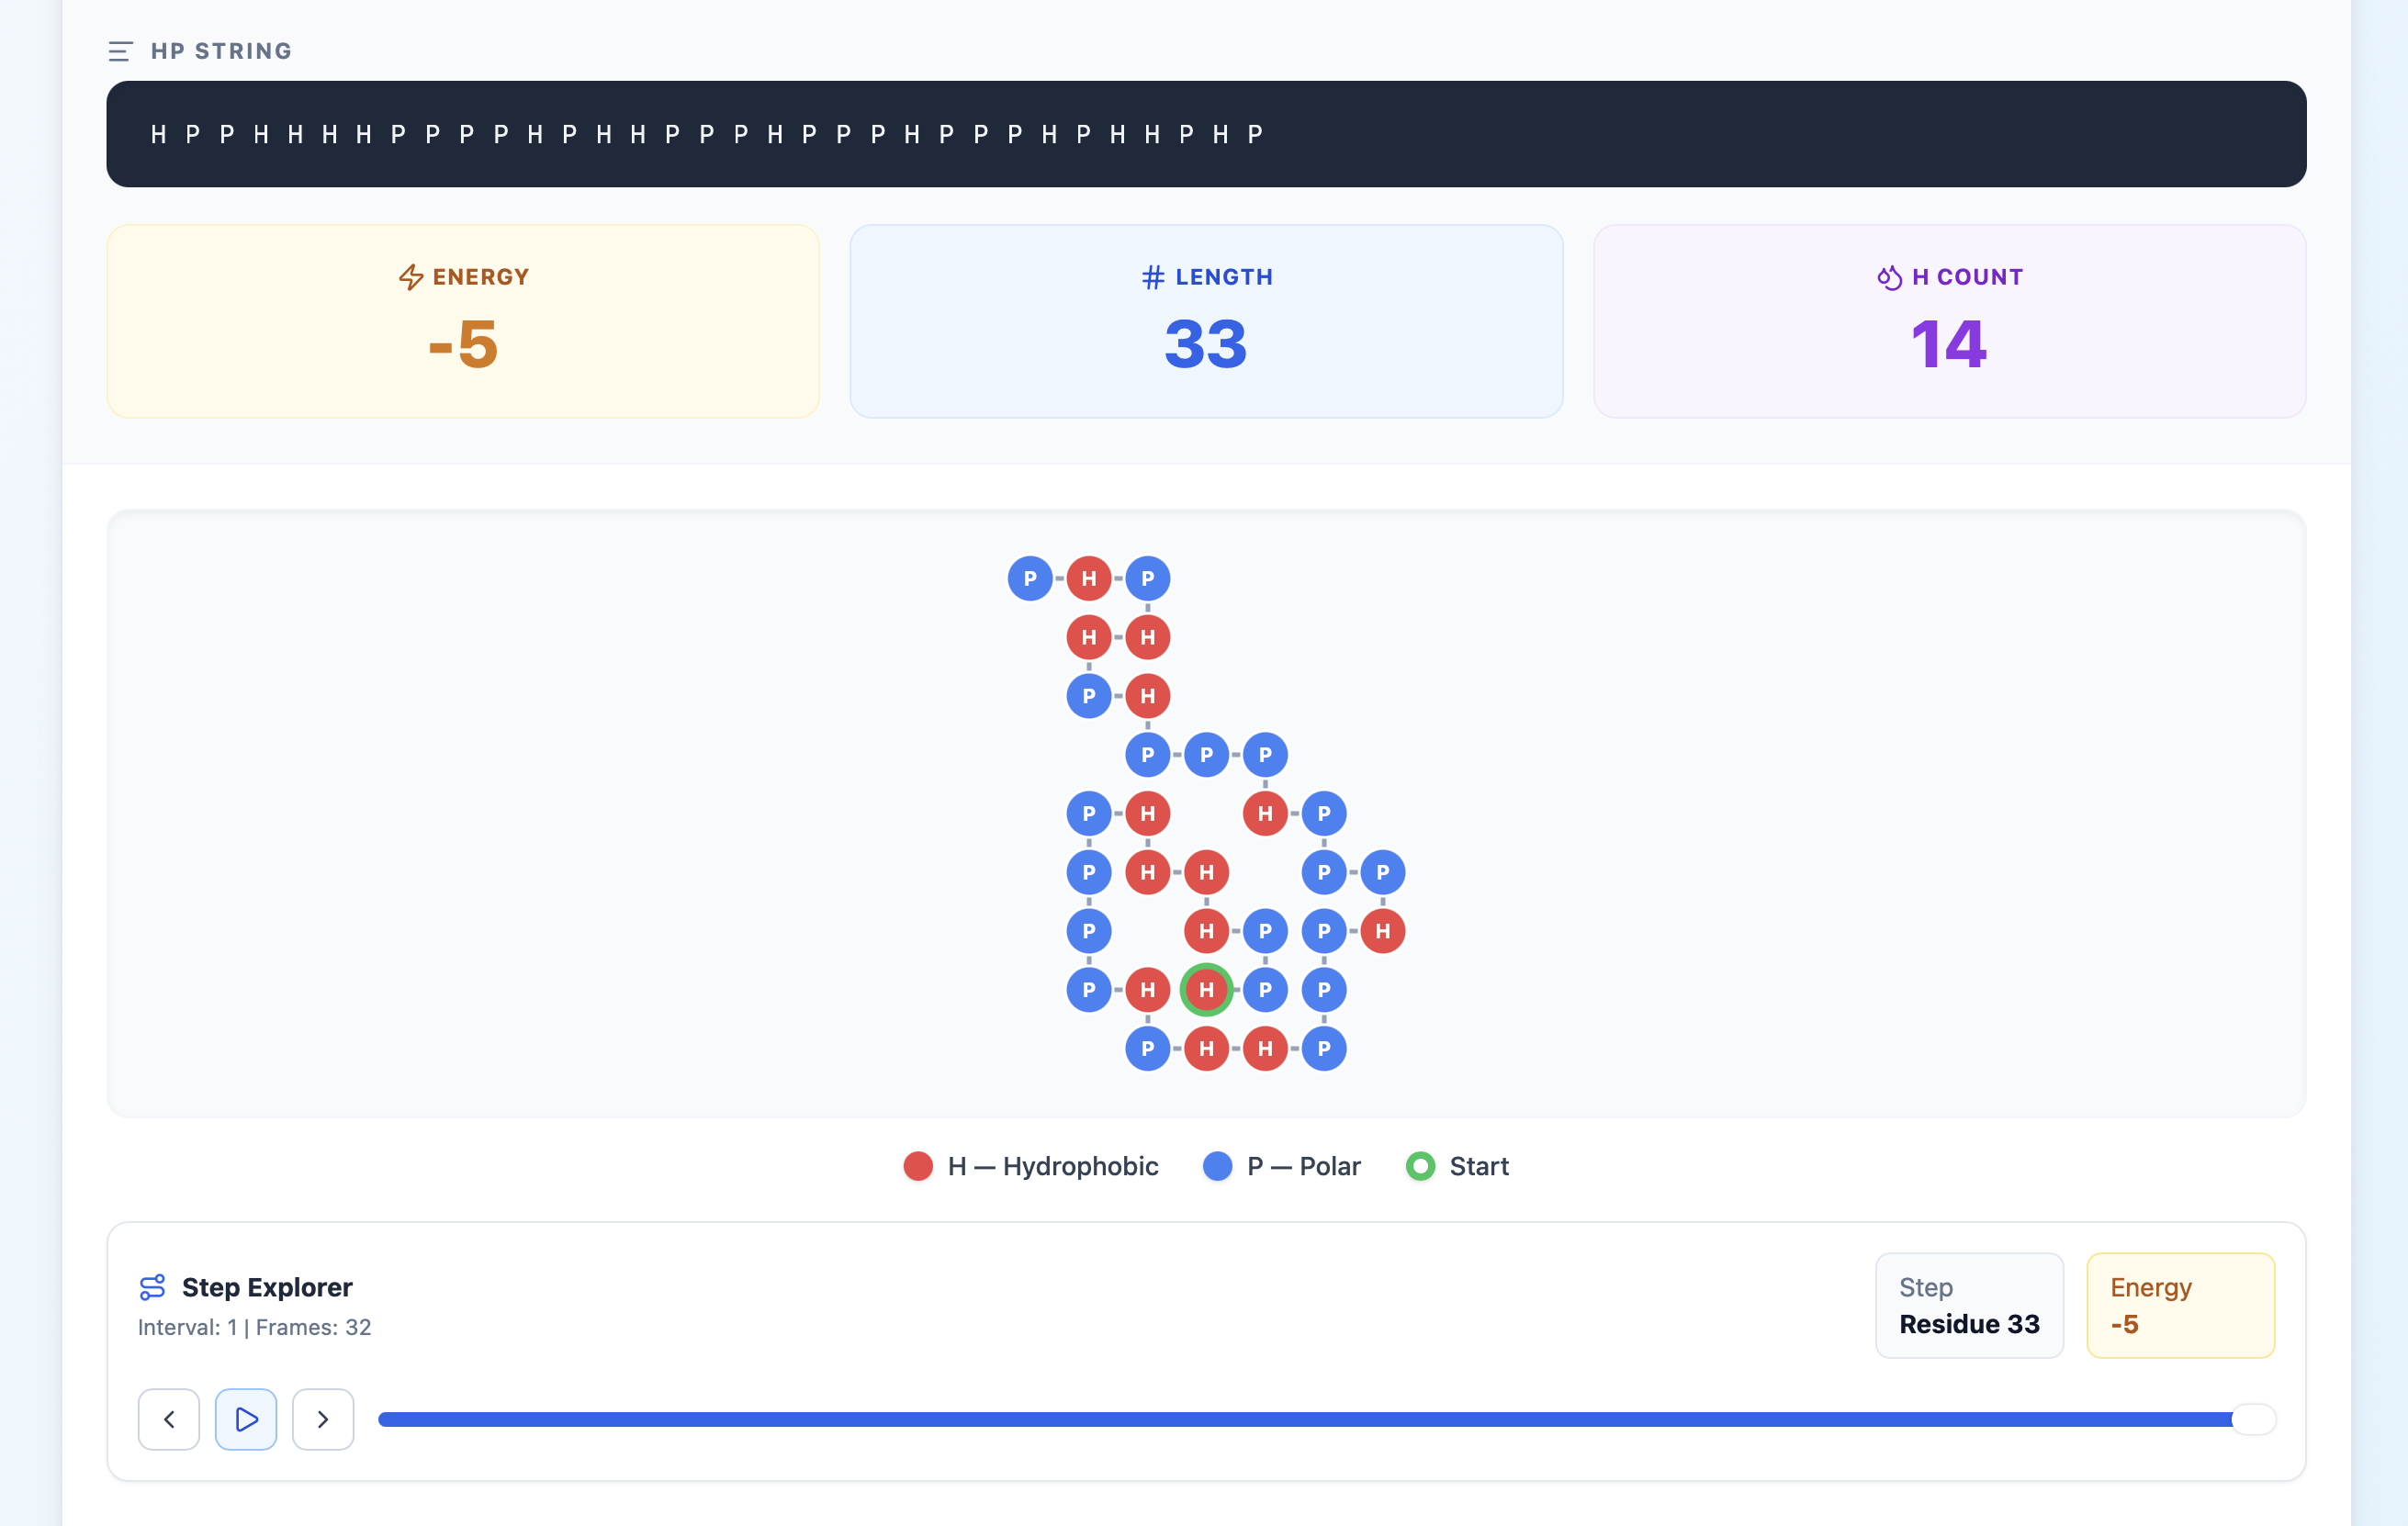
\includegraphics[width=\textwidth,height=0.70\textheight,keepaspectratio]{Figuras/2dStructure5.png}
\caption[2D HP step explorer: final frame]{Final 2D HP structure generated by the platform. The completed lattice conformation is shown together with the HP string, final energy, sequence length, hydrophobic residue count, and final step-explorer position.}
\label{fig:appendix_2d_structure_step_final}
\end{figure}
\FloatBarrier

\begin{figure}[!htbp]
\centering
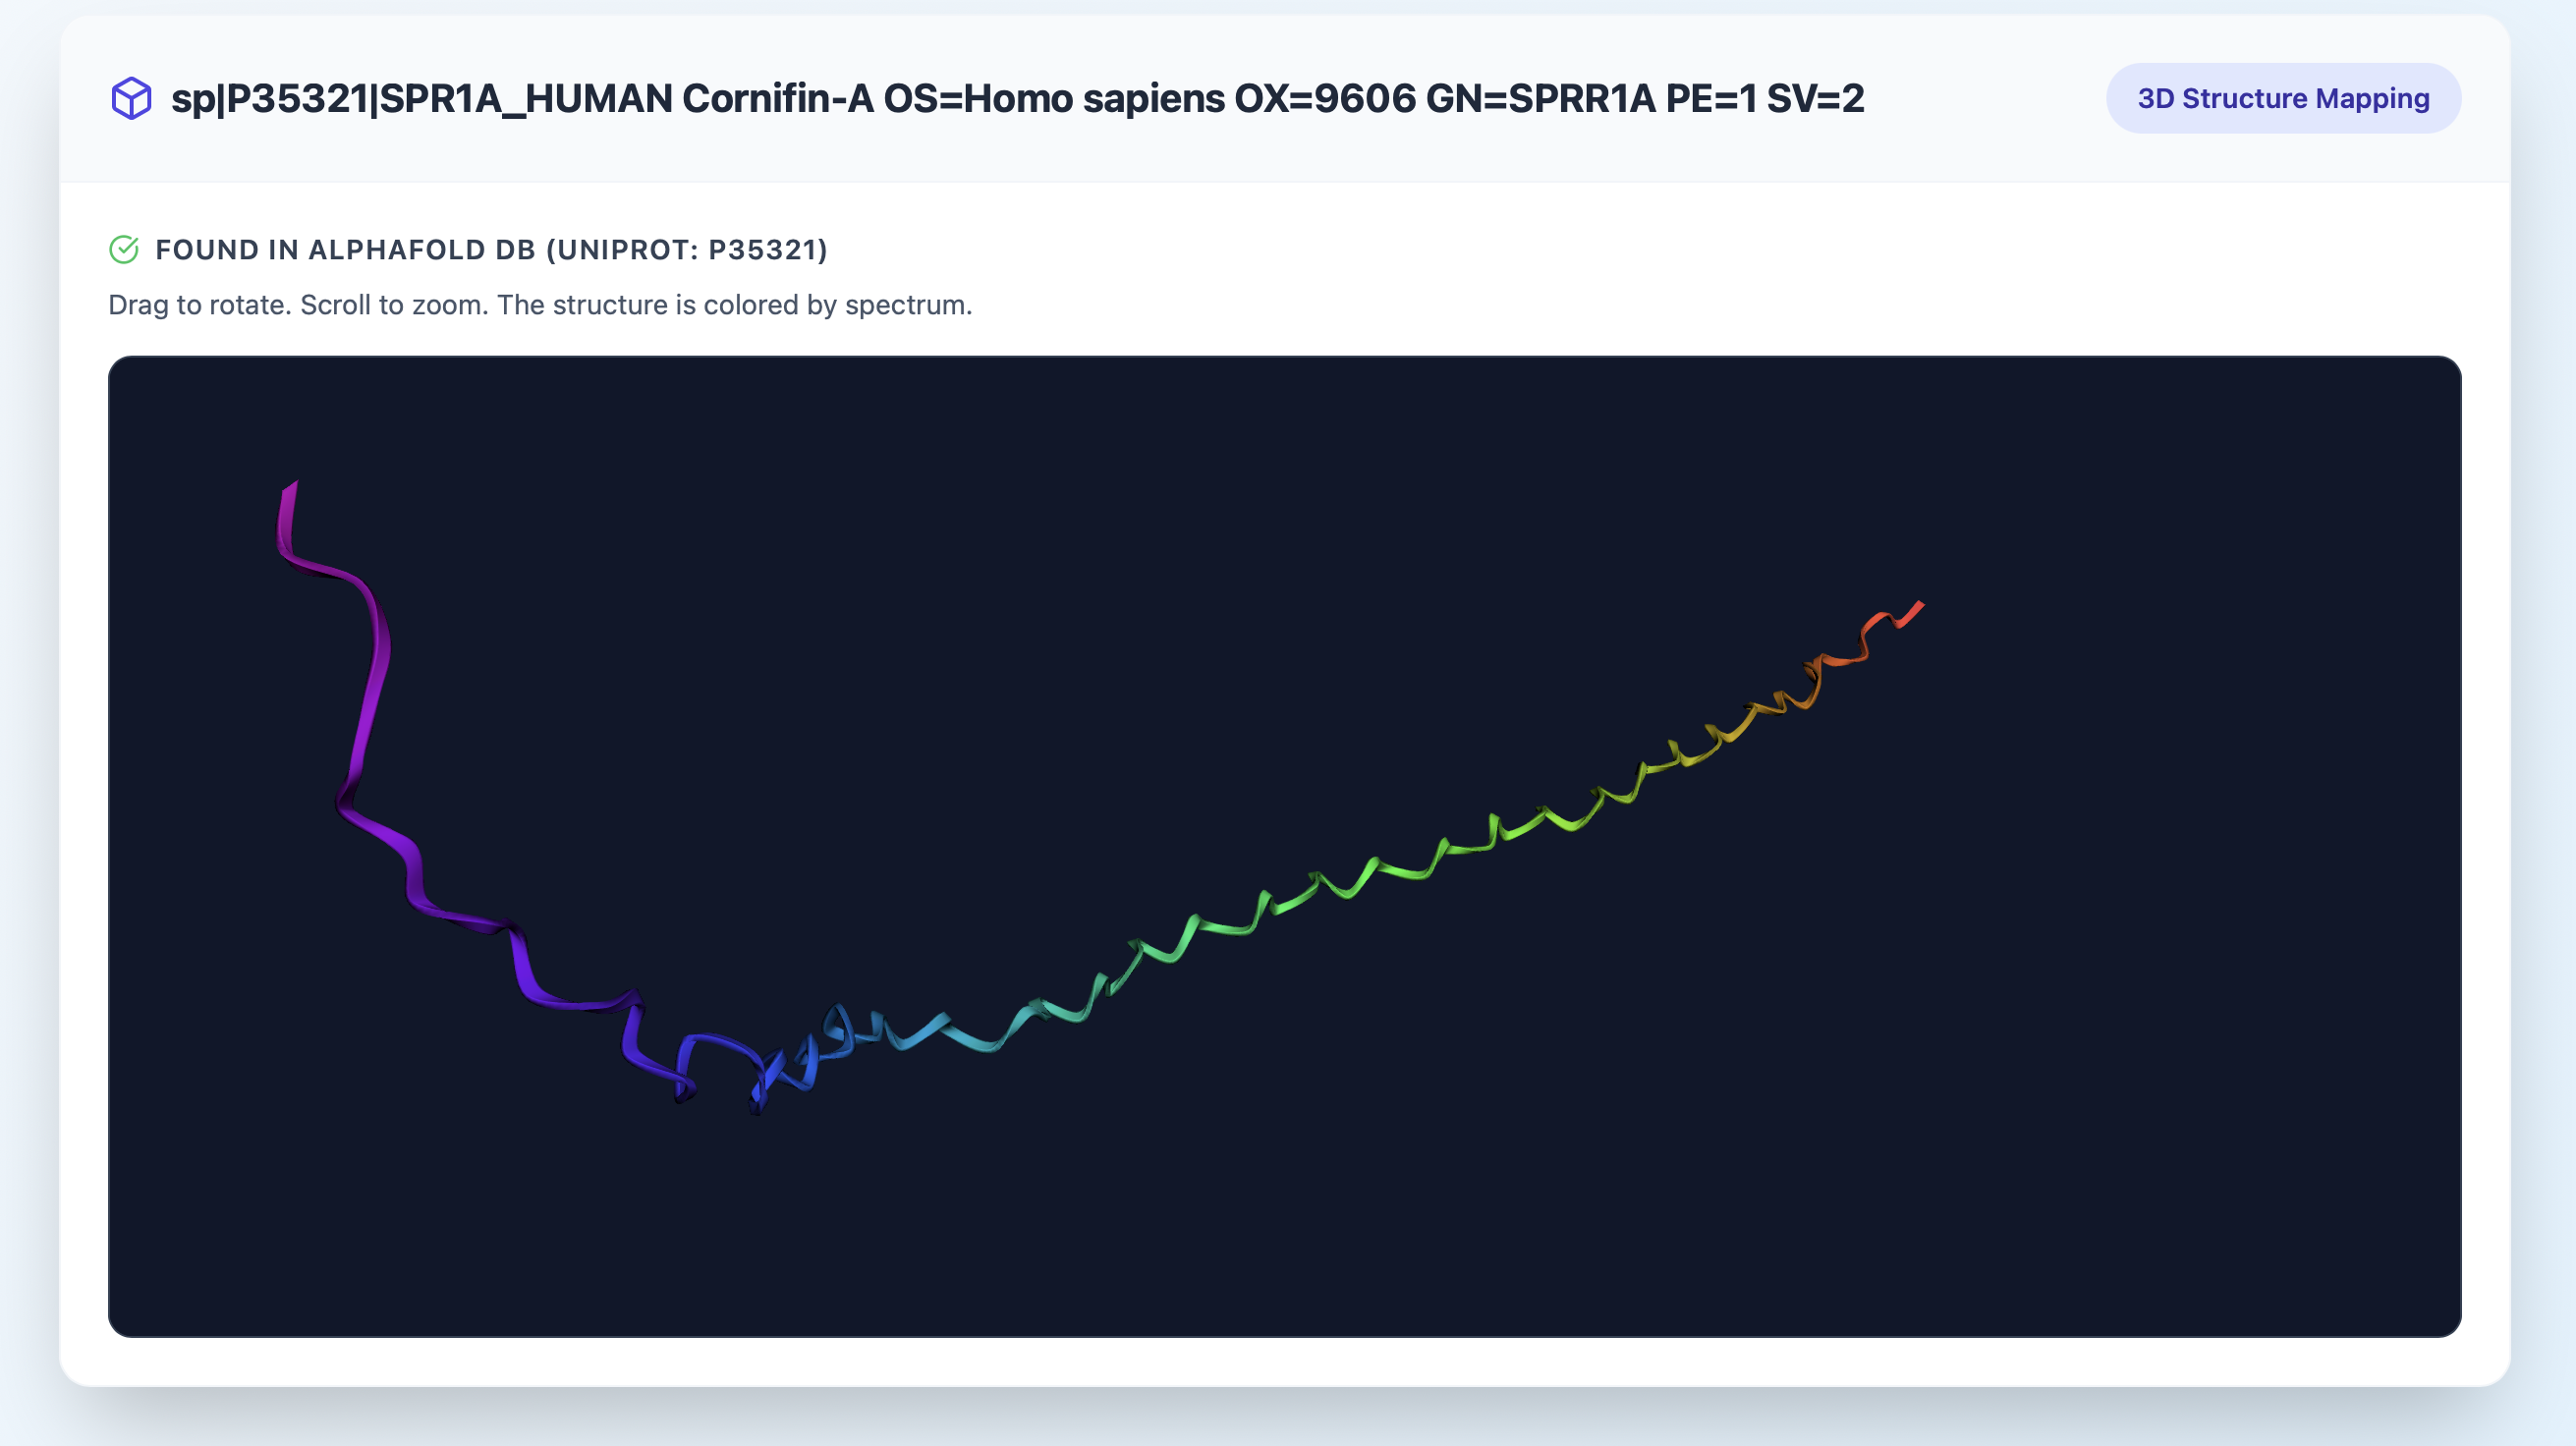
\includegraphics[width=\textwidth,height=0.76\textheight,keepaspectratio]{Figuras/3dStructureView.png}
\caption[3D structure visualization screen]{3D structure visualization screen. The platform retrieves known structures from AlphaFold DB or falls back to ESMFold for sequence-based prediction when necessary.}
\label{fig:appendix_3d_structure}
\end{figure}
\FloatBarrier
% !TEX root = ../main.tex


\newpage

\thispagestyle{empty}

% Última página
\input{Setup/ultima_pagina}

\end{document}
